\twocolumn

\chapter{Гидрометеорология на яхте}

Успех морского плавания, особенно на парусном судне, в значительной
степени зависит от погоды, т.е. от состояния атмосферы у земной
поверхности в данный момент и на данном месте. Явления природы,
создающие погоду на море, рассматривают две смежные науки:
метеорология, изучающая земную атмосферу и происходящие в ней
физические явления и процессы, и океанология, исследующая, в
частности, физические свойства водной среды (гидросферы).

К основным метеорологическим элементам атмосферы, определяющим её
физическое состояние и процессы, происходящие в ней, относятся:
атмосферное давление, температура и влажность воздуха, облачность,
осадки, видимость и ветер. В океанологии элементами, так или иначе
влияющими на состояние погоды, считаются такие гидрологические
явления, как волнение, морские течения (в том числе и
приливно\-/отливные), температура, солёность и плотность воды.

В отличие от общей гидрометеорологии, которая занимается изучением
перечисленных элементов и их взаимодействия, навигационная
гидрометеорология носит более узкий характер. Её задача \--- помочь
мореплавателю разбираться в гидрометеорологической обстановке, уметь
её анализировать, правильно, по инструментальным и визуальным
наблюдениям оценивать состояние погоды на ближайшее время и, используя
официальные прогнозы по радио, уметь определять ожидаемую погоду по
местным признакам.

\section{Атмосферное давление}

Основным элементом при прогнозировании погоды в море можно считать
атмосферное давление. Старинная морская поговорка довольно длительно
говорит об этом:

\begin{quote}
Если барометра\index{барометр} стрелки падение \\
Требует в море вниманья и бдения, \\
То штурман тогда лишь спокойно заснёт, \\
Когда он высоко и кверху идёт. \\
\end{quote}

Физическая сущность атмосферного давления \--- это вес столба воздуха
от верхней границы атмосферы до земной (водной) поверхности. Плотность
воздуха постоянно меняется от колебаний температуры и влажности и от
давления верхних слоев атмосферы на нижние. Вместе с изменением
плотности воздуха меняется его вес и атмосферное давление.

Нормальным атмосферным давлением принято считать массу ртутного столба
высотой 760 мм на площади 1~см$^2$, находящейся на уровне Мирового
океана (уровне моря), при температуре 0\grC и на широте места 45\gr.

В практике метеорологических наблюдений атмосферное давление
измеряется миллиметрами ртутного столба, или миллибарами
(мбар). Специальные таблицы для перевода единиц атмосферного давления
имеются в <<Мореходных таблицах>> (МТ-75).

Для измерения давления в судовых условиях применяют два прибора \---
барометр\-/анероид\index{барометр-анероид} и барограф\index{барограф}.

Шкала \textbf{анероида}\index{барометр-анероид} (рис.~\ris{109})
градуирована в миллиметрах ртутного столба, а в последние годы \--- в
гектопаскалях (гПа) (по международной системе единиц (СИ) стандартное
атмосферное давление составляет 1013,247~гПа = 1013,247~мбар =
760~мм~рт.~ст.). На яхте анероид должен храниться в горизонтальном
положении.

Показания анероида снимают, не вынимая его из футляра, и исправляют их
тремя поправками, которые находят в паспорте прибора:

\begin{enumerate}
\item Поправка шкалы \--- по величине давления. 
\item Поправка на температуру прибора получается при умножении
  температурного коэффициента <<$c$>> на температуру прибора <<$t$>>
  по формуле $d = c \cdot t$.
\item Добавочная поправка \--- на механическое состояние пружины
  анероида и барокоробки. Эта поправка должна иметь дату определения в
  паспорте.
\end{enumerate}

\begin{figure}[!htb]
  \centering{}
  \includegraphics[scale=1.2]{0109P}
  \caption{Барометр-анероид}
  \label{fig:109}
  \small
  \centering{}
  1 \--- пружина; 2 \--- анероидная коробка; 3 \--- термометр\-/атташе; 4 \--- отсчёт 778,5~мм. 
\end{figure}

Для удобства определения поправки на температуру прибора в анероид
включён полукруглый \textit{<<термометр\-/атташе>>}
\index{термометр-атташе}. Так как поправки анероида могут время от
времени изменяться, то перед выходом в плавание его необходимо
проверить.

\textbf{Барограф}\index{барограф} \--- прибор, ведущий непрерывную запись атмосферного
давления на специальной бумажной ленте \--- \textbf{барограмме}\index{барограмма}
(рис.~\ris{110}). Он удобен тем, что позволяет судить об изменении
атмосферного давления во времени, или, как говорят, о
\textbf{барометрической}\index{барометрическая тенденция}
\index{барическая тенденция} (барической) \textbf{тенденции}. Барабан, на
который надевается барограмма, имеет часовой механизм с заводом, при
котором лента совершает полный оборот в течение недели. Барограмма
имеет сетку, на которой нанесены по горизонтали временные интервалы
\--- часы и сутки, а по вертикали \--- давление в миллибарах.

Меняют ленту раз в неделю. При этом на обороте новой барограммы
необходимо записывать дату, время начала записи (с точностью до
минуты) и координаты яхты. Начало записи должно точно соответствовать
моменту записи по судовым часам. В это же время заводят часовой
механизм барографа. Держать барограф можно на отдельной полочке или
прямо на штурманском столе. В обоих случаях прибор нужно страховать от
падения при крене или на волнении. Ставить барограф следует на
амортизирующую прокладку (поролон или губчатую резину).

Барометрическую тенденцию (рис.\ris{111}) определяют по характеру
кривой на барограмме, как правило, за последние три часа.

\begin{figure*}[!htb]
  \centering{}
  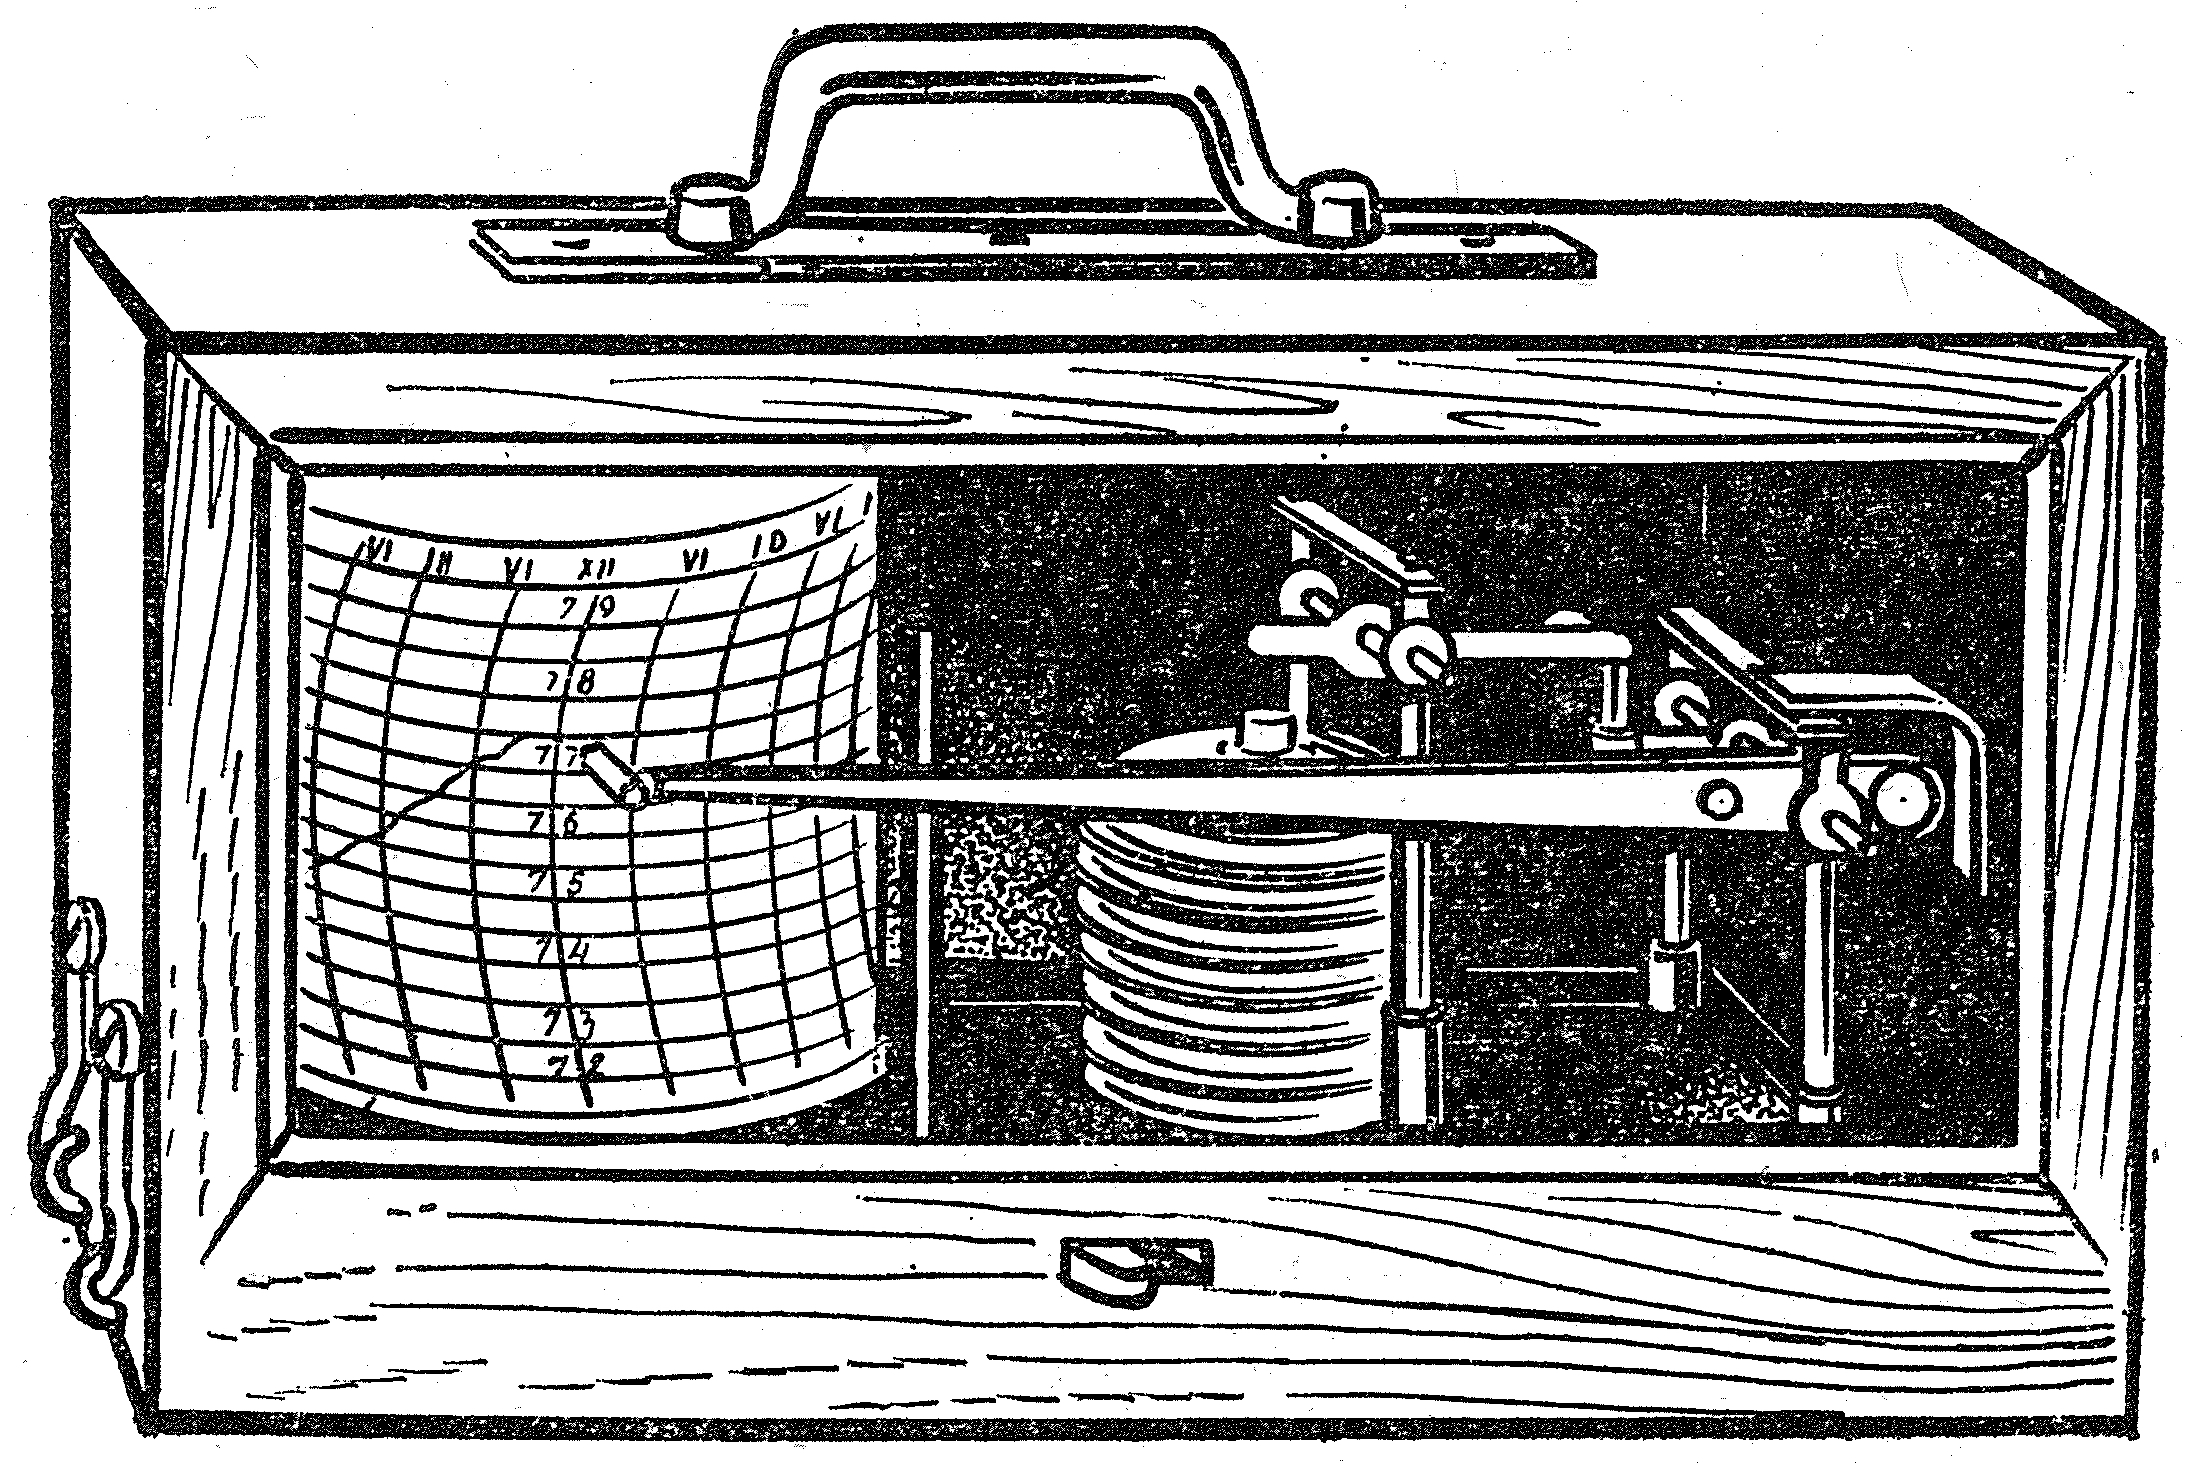
\includegraphics[width=0.8\linewidth]{0110P}
  \caption{Барограф \No 4}
  \label{fig:110}
\end{figure*}

\begin{figure*}[!htb]
  \centering{}
  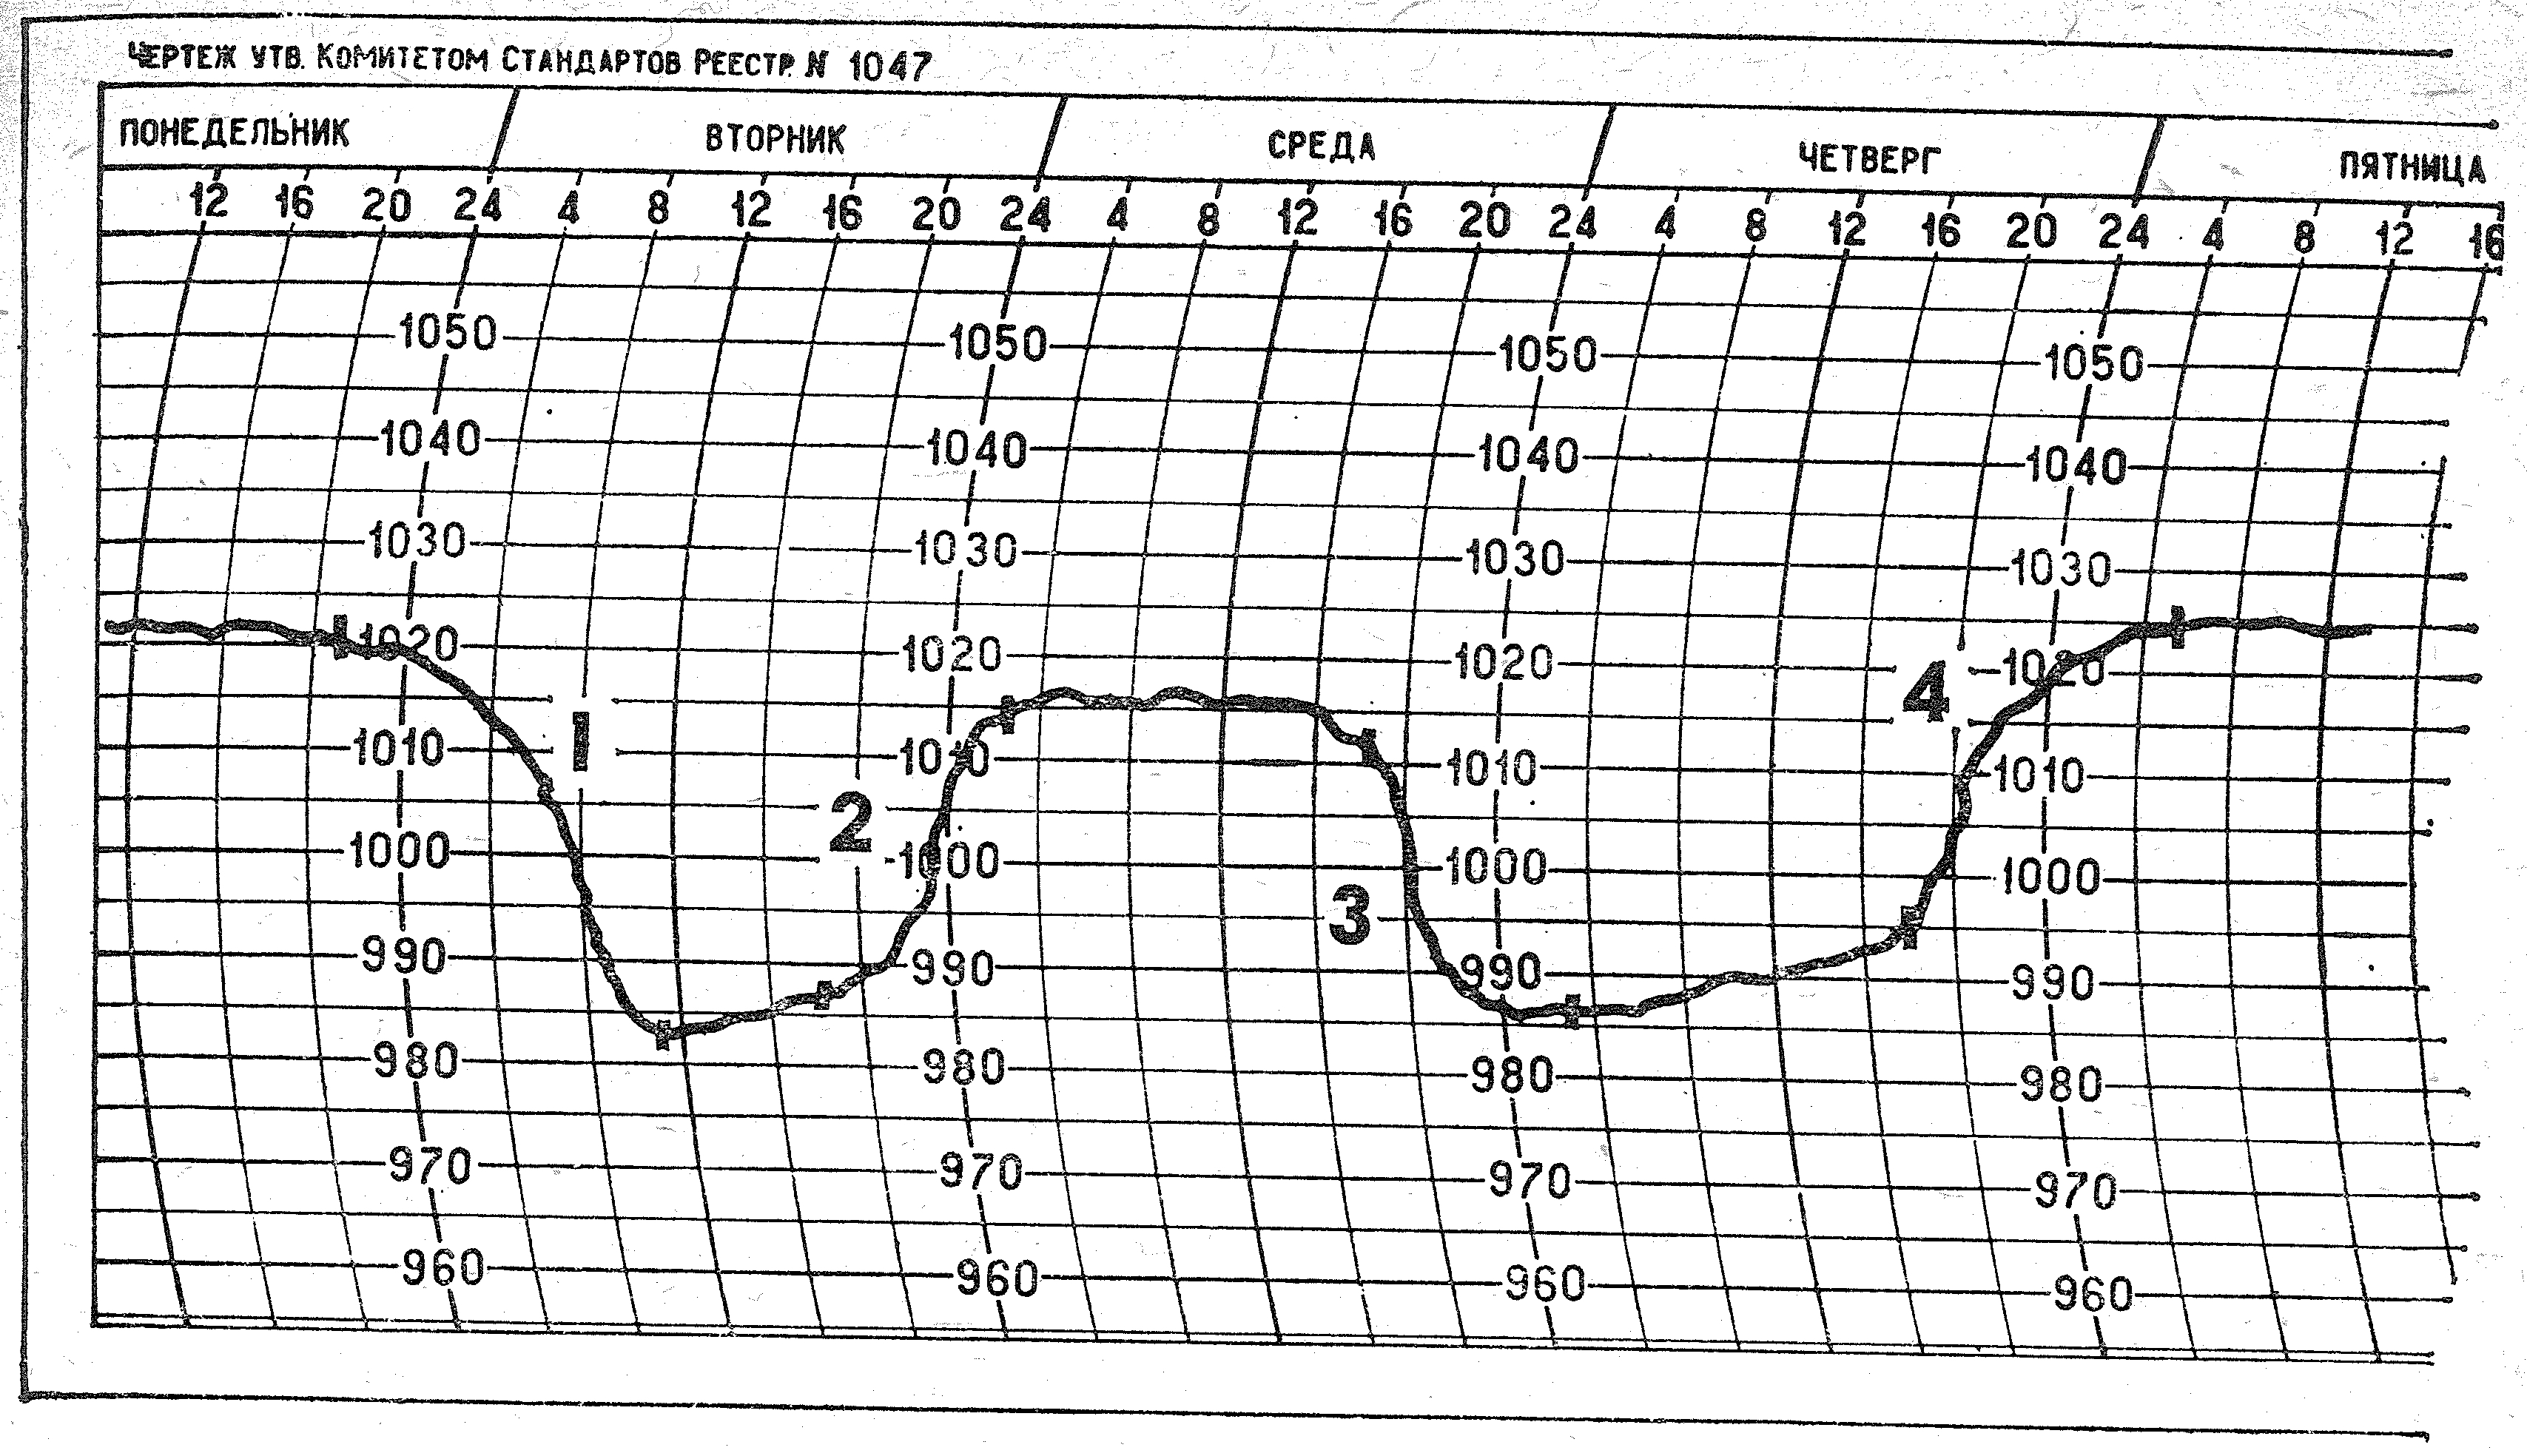
\includegraphics[width=\linewidth]{0111P}
  \caption{Примеры барических тенденций}
  \label{fig:111}
  \small \centering{} Кривая выпуклостью вверх: при падении давления
  \--- значительное ухудшение погоды (1), при повышении \--- к
  улучшению погоды (4). Кривая выпуклостью вниз: при падении давления
  \--- ослабление ветра, некоторое улучшение погоды (3); при повышении
  \--- может усилиться ветер (2)
\end{figure*}

В суточном ходе атмосферного давления имеется два максимума \--- около
10 и 22 часов и два минимума \--- около 4 и 16 часов.

Показания барометра\index{барометр} обычно записывают в судовой журнал при смене вахт,
а при неустойчивой погоде \--- не реже чем через 2 часа. В последнем
случае давление надо наблюдать чаще и при резком изменении его падения
запись делается сразу же.

На справочных или синоптических картах точки с одинаковым атмосферным
давлением соединены сплошными линиями \--- изобарами. Все нанесённые
на карту изобары составляют барическое поле\index{барическое поле} данного района. Отдельные
участки барического поля, отличающиеся своей конфигурацией и типичной
разностью давлений, называют барическими системами \--- областями с
замкнутыми или незамкнутыми изобарами, с повышенным или пониженным
атмосферным давлением.

Различают две замкнутые (основные) барические системы\index{барическая система}:

\begin{description}
\item[циклон] \index{циклон} \index{барический минимум} (барический минимум) \--- область, ограниченная
  концентрически замкнутыми изобарами, давление в которой понижается
  от периферии к центру, где наблюдается самое низкое давление (в
  умеренных широтах \--- 990\otdo 1005~мбар);
\item[антициклон] \index{антициклон} \index{барический максимум} (барический максимум) \--- область, также
  ограниченная изобарами, но отличающаяся от циклона тем, что высокое
  атмосферное давление в центре антициклона уменьшается к его
  периферии.
\end{description}

Незамкнутые изобары складываются в три барические системы:

\begin{description}
\item[ложбина]\index{антициклон!ложбина} \--- область низкого давления, отходящая от циклона; 
\item[гребень]\index{антициклон!гребень} \--- область высокого давления, отходящая от антициклона; 
\item[седловина]\index{антициклон!седловина} \--- барическая система, расположенная крестообразно между соседними двумя циклонами и двумя антициклонами.
\end{description}

\section{Температура воздуха}

\index{температура воздуха}Температура воздуха в нижних слоях атмосферы складывается в основном
из температуры подстилающей поверхности - земли или воды, получающей
основную часть тепловой энергии солнца. Тепло приземных слоев воздуха
верхним передаётся двумя путями:

\begin{itemize}
\item непосредственным вертикальным смешиванием тёплых нижних слоев с
  верхними в результате \textbf{конвекции}, т.\=,е. когда тёплый
  воздух поднимается вверх, а более холодный воздух верхних или
  соседних слоев заменяет его. Над морем конвекция всегда усиливается
  ночью, при незначительном изменении температуры воды и более сильном
  охлаждении верхних слоев воздуха;
\item вихреобразным, т.\=,е. \textbf{турбулентным}, беспорядочным
  движением воздушных масс, переносящих тепло в самых различных
  направлениях.
\end{itemize}

Температура воздуха зависит и от состояния погоды. При сплошной
облачности перепады температуры значительно меньше, чем при ясном
небе. Во время дождя и после него температура может понижаться.

Наконец, зависит температура воздуха и от широты местности: в тропиках
теплее, чем в умеренных или высоких широтах.

При наблюдении за температурой различают её суточный и годовой ход.

В спортивном мореплавании практическое значение имеет суточный ход
т.\=,е. изменение температуры в течение суток в определённом
районе. Обычно суточный ход температуры воздуха над морем достигает
минимума через 2\otdo 3 часа после восхода солнца, а максимума \--- к
15\otdo 16 часам. Такой суточный ход характерен лишь для устойчивой
хорошей погоды. Нарушается он при теплообменных процессах в атмосфере,
например при смене тёплых воздушных масс холодными. В таких случаях
ночная температура может оказаться выше дневной.

\textbf{Суточная амплитуда температуры
  воздуха}\index{температура воздуха!амплитуда суточная} \--- разность между
самой высокой и самой низкой температурой за сутки зависит также от
облачности, при которой она уменьшается, и от времени года. В открытых
морях и океанах суточная амплитуда составляет около 1,0\otdo 1,5\grC,
а в закрытых морях может достигать 10\otdo 15\grC. Все это необходимо
учитывать, так как характер суточного хода имеет прямое отношение к
погоде. Так, нарушение правильного суточного хода температуры
предвещает ухудшение погоды, а при резком понижении дневной
температуры после ненастья можно ждать улучшения погоды. Ухудшение
погоды может наступить и при повышении температуры к вечеру.

\section{Влажность воздуха, облачность, осадки}

Источником влаги в воздухе является вода, испаряющаяся с подстилающей
поверхности океанов, морей, озёр, рек, водохранилищ. Эта влага
находится в атмосфере в трёх состояниях: газообразном \--- в виде
пара, жидком \--- в виде разной величины капель и твёрдом \--- в виде
снега, града и других ледяных образований. Поскольку водяной пар \---
составная часть атмосферы, он существенно влияет на все атмосферные
процессы.

Влажность воздуха
\index{влажность воздуха}
\index{влажность воздуха!абсолютная}
\index{влажность воздуха!относительная}
определяется наличием в нем водяного пара, и зависит она от количества
его массы, в метеорологии учитывают два вида влажности: абсолютную,
выраженную массой водяного пара, содержащегося в единице объёма
воздуха (кг/м$^3$), и относительную, выраженную отношением абсолютной
влажности к её максимальному значению при данной температуре. При
100\,\% относительной влажности в воздухе может произойти конденсация
водяных паров с выпадением воды. Температура, при которой это
случается, называется точкой росы.

Наглядный пример жидкого и твёрдого состояния влаги в атмосфере \---
облака, состоящие из мельчайших капелек воды, кристалликов льда или их
смеси. Необходимое условие образования облаков \--- насыщение водяных
паров до состояния \textbf{конденсации} (превращение пара в воду) или
\textbf{сублимации} (превращение пара в ледяные кристаллы, минуя
жидкую фазу) и понижение температуры воздуха до критической. Кроме
того, в воздухе должны находиться так называемые \textbf{ядра
  конденсации} (или сублимации). Основная масса ядер конденсации
состоит из частиц соли, попавших в атмосферу из испаряющихся водной
пыли и брызг во время штормов. Взвешенные в воздухе частицы соли
переносятся воздушными потоками до встречи с водяными
капельками. Ядрами конденсации могут быть и микроскопические частицы
пыли и дымообразующих веществ. Переохлаждённые капельки с ядер
конденсации, замерзающие при низких температурах, могут
сублимироваться и образовывать ледяные кристаллики.

В основу классификации облачных структур взяты латинские слова,
характеризующие их внешний вид: стратус (\textit{stratus}) - слой,
кумулюс (\textit{cumulus}) - куча, циррус (\textit{cirrus}) - перо,
альтус (\textit{altus}) - высокий, опакус (\textit{opakus}) - плотный,
нимбус (\textit{nimbus})- дождь, транслюцидус (\textit{translucidus})
- просвечивающий, фрактус (\textit{fractus}) - разорванный, хумилис
(\textit{humilis}) - низкий.

\begin{savenotes}
\afterpage{
\begin{figure}
  \centering
  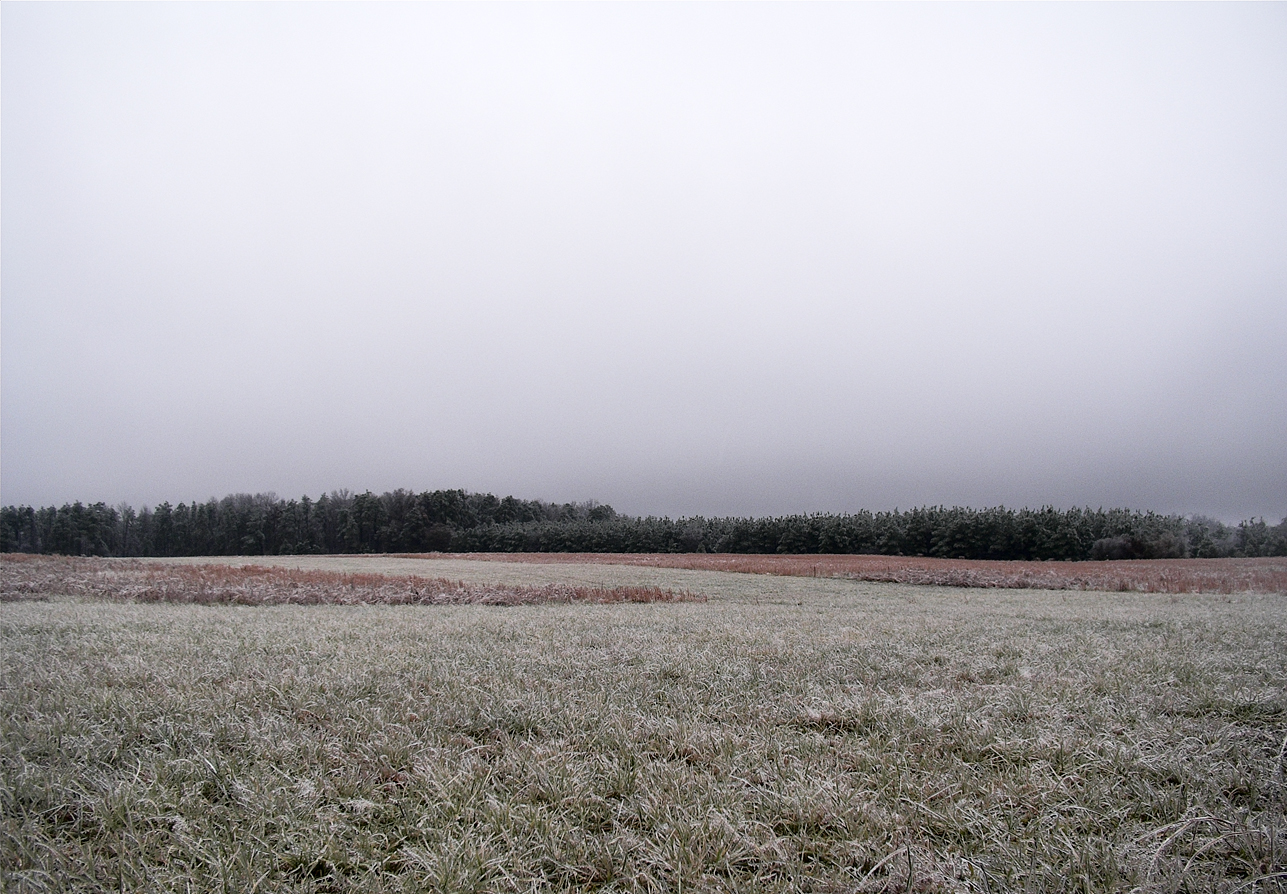
\includegraphics[width=\linewidth]{clouds/stratus_opacus_uniformis}
  \caption[Stratus opacus uniformis]{Stratus opacus uniformis\protect\footnote{\url{https://commons.wikimedia.org/wiki/File:Stratus-Opacus-Uniformis.jpg}}}
  \label{fig:stratus}
\end{figure}

\begin{figure}
  \centering
  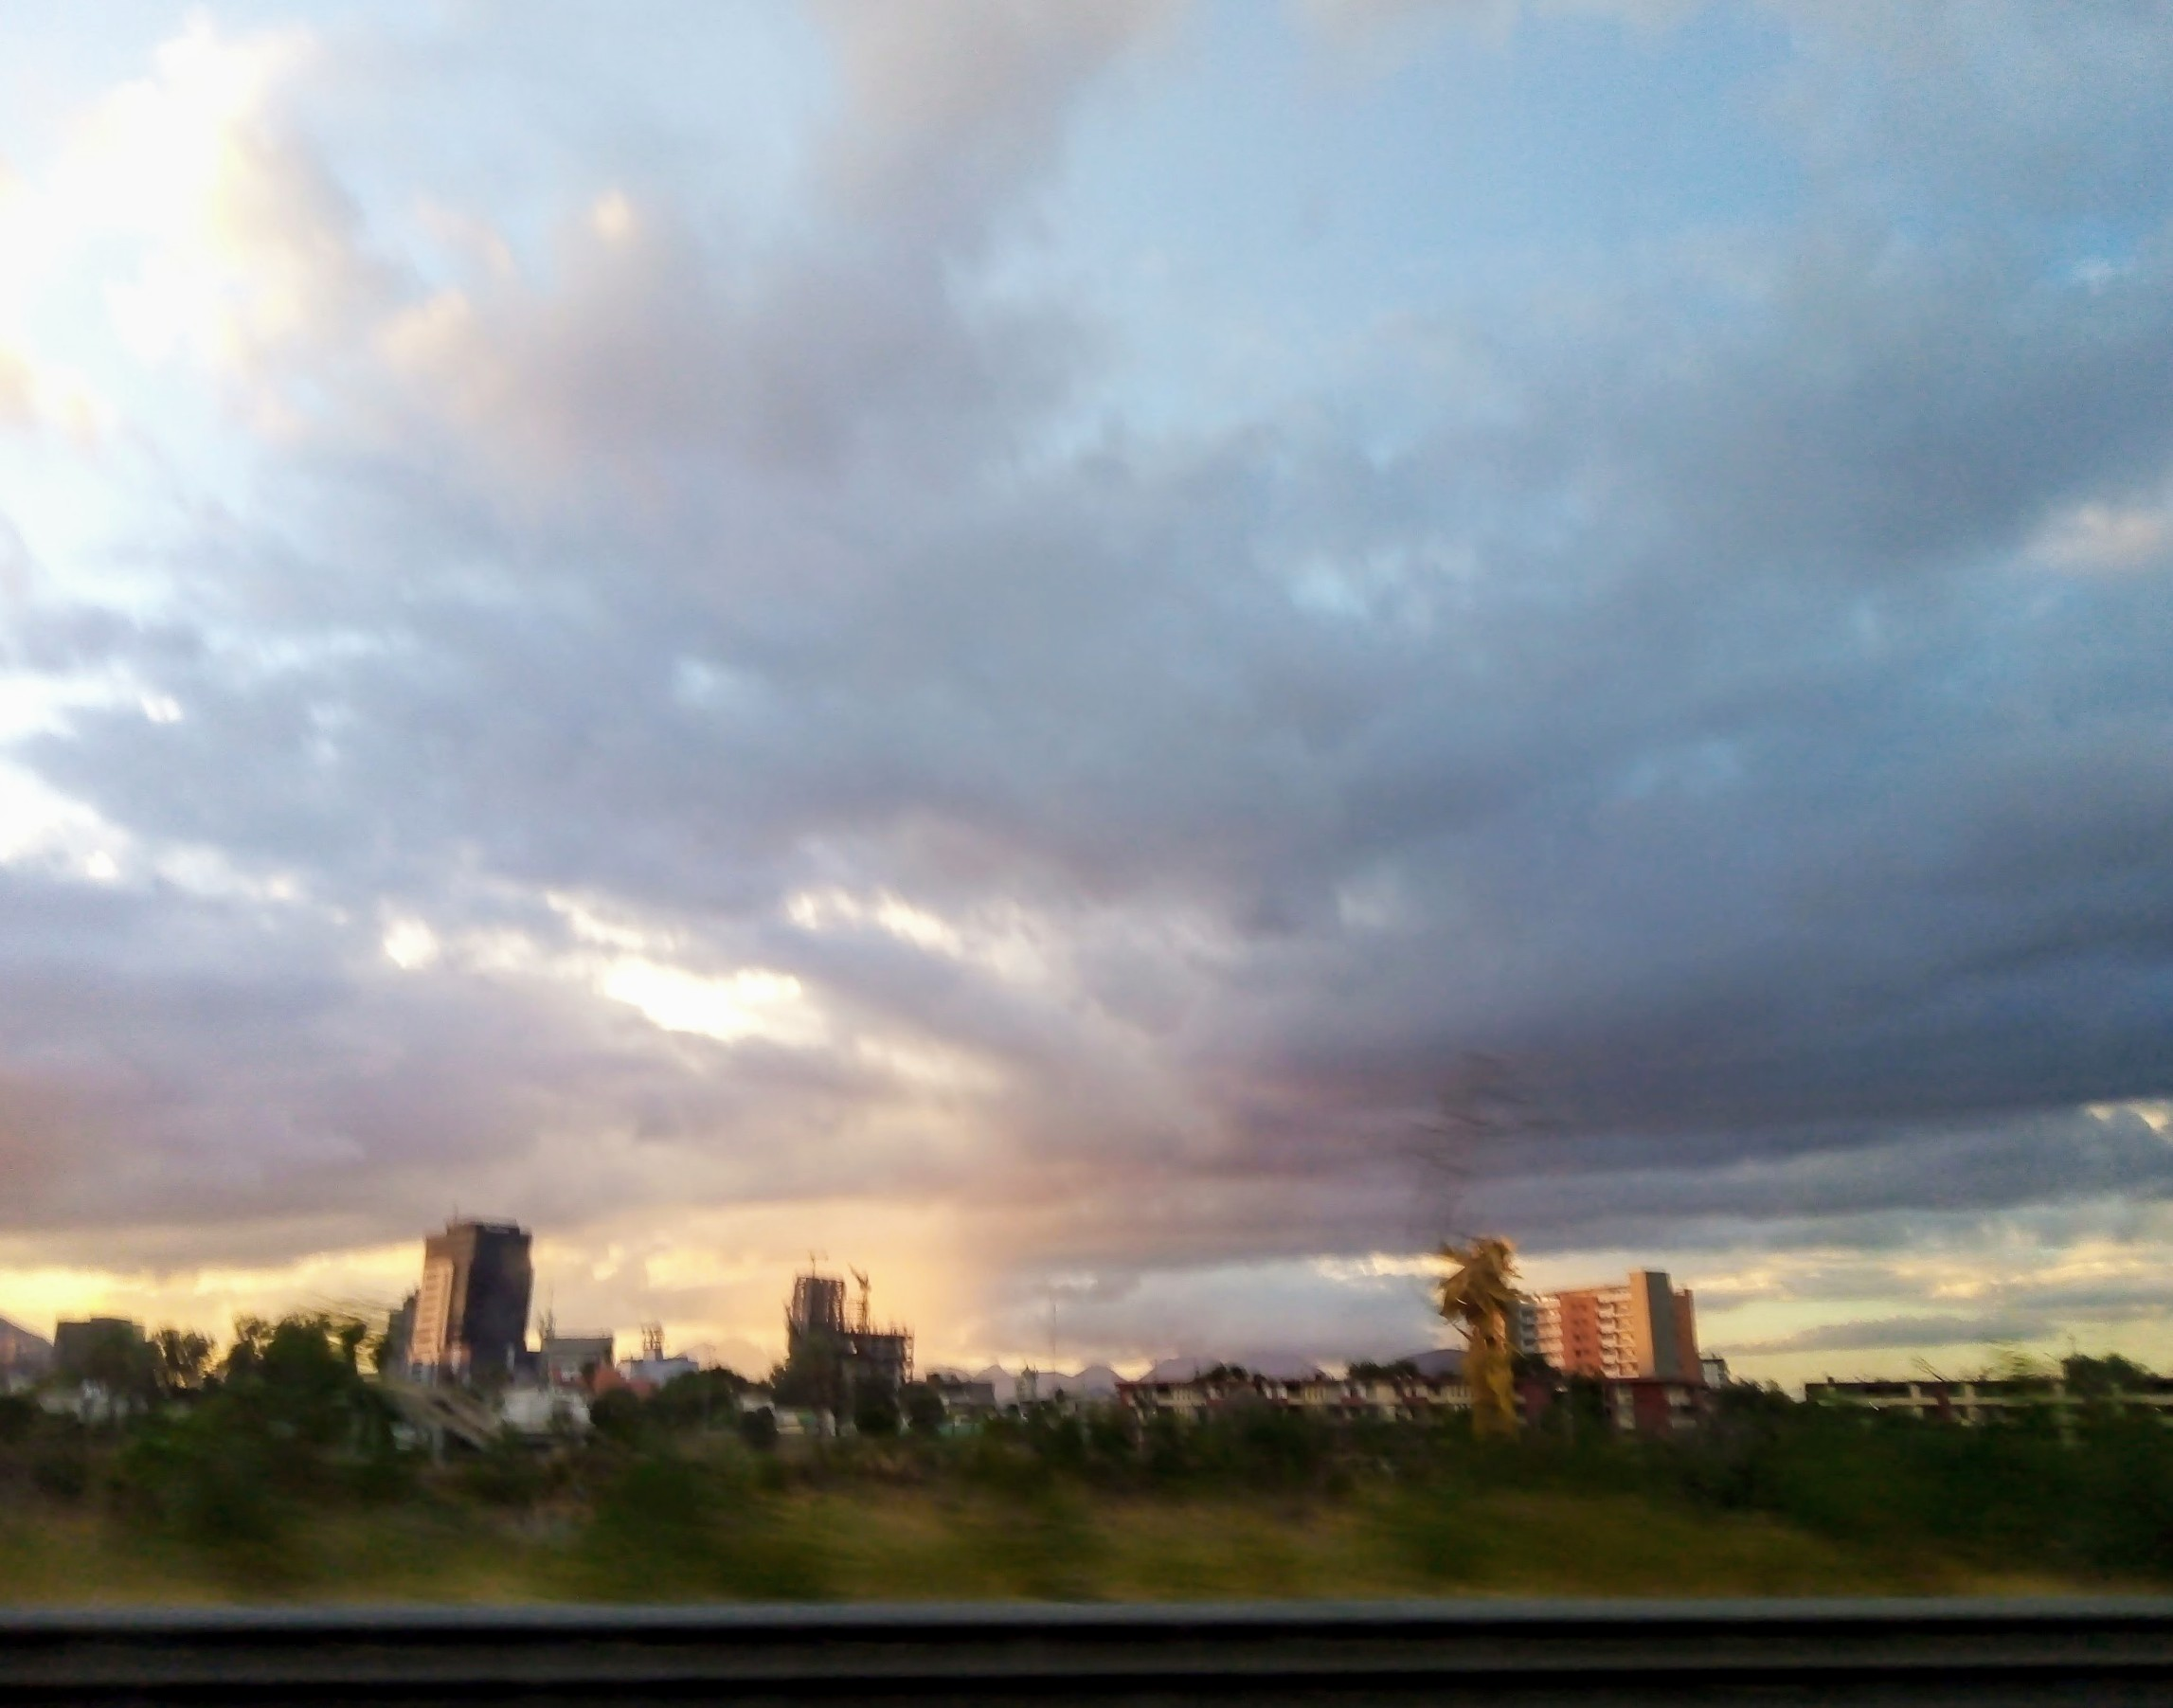
\includegraphics[width=\linewidth]{clouds/stratocumulus_opacus}
  \caption{Stratocumulus opacus}
  \label{fig:stratocumulus-opacus}
  Источник\footnote{\url{https://commons.wikimedia.org/wiki/File:Stratocumulus_stratiformis_opacus_praecipitatio_1.jpg}}
\end{figure}

\begin{figure}
  \centering
  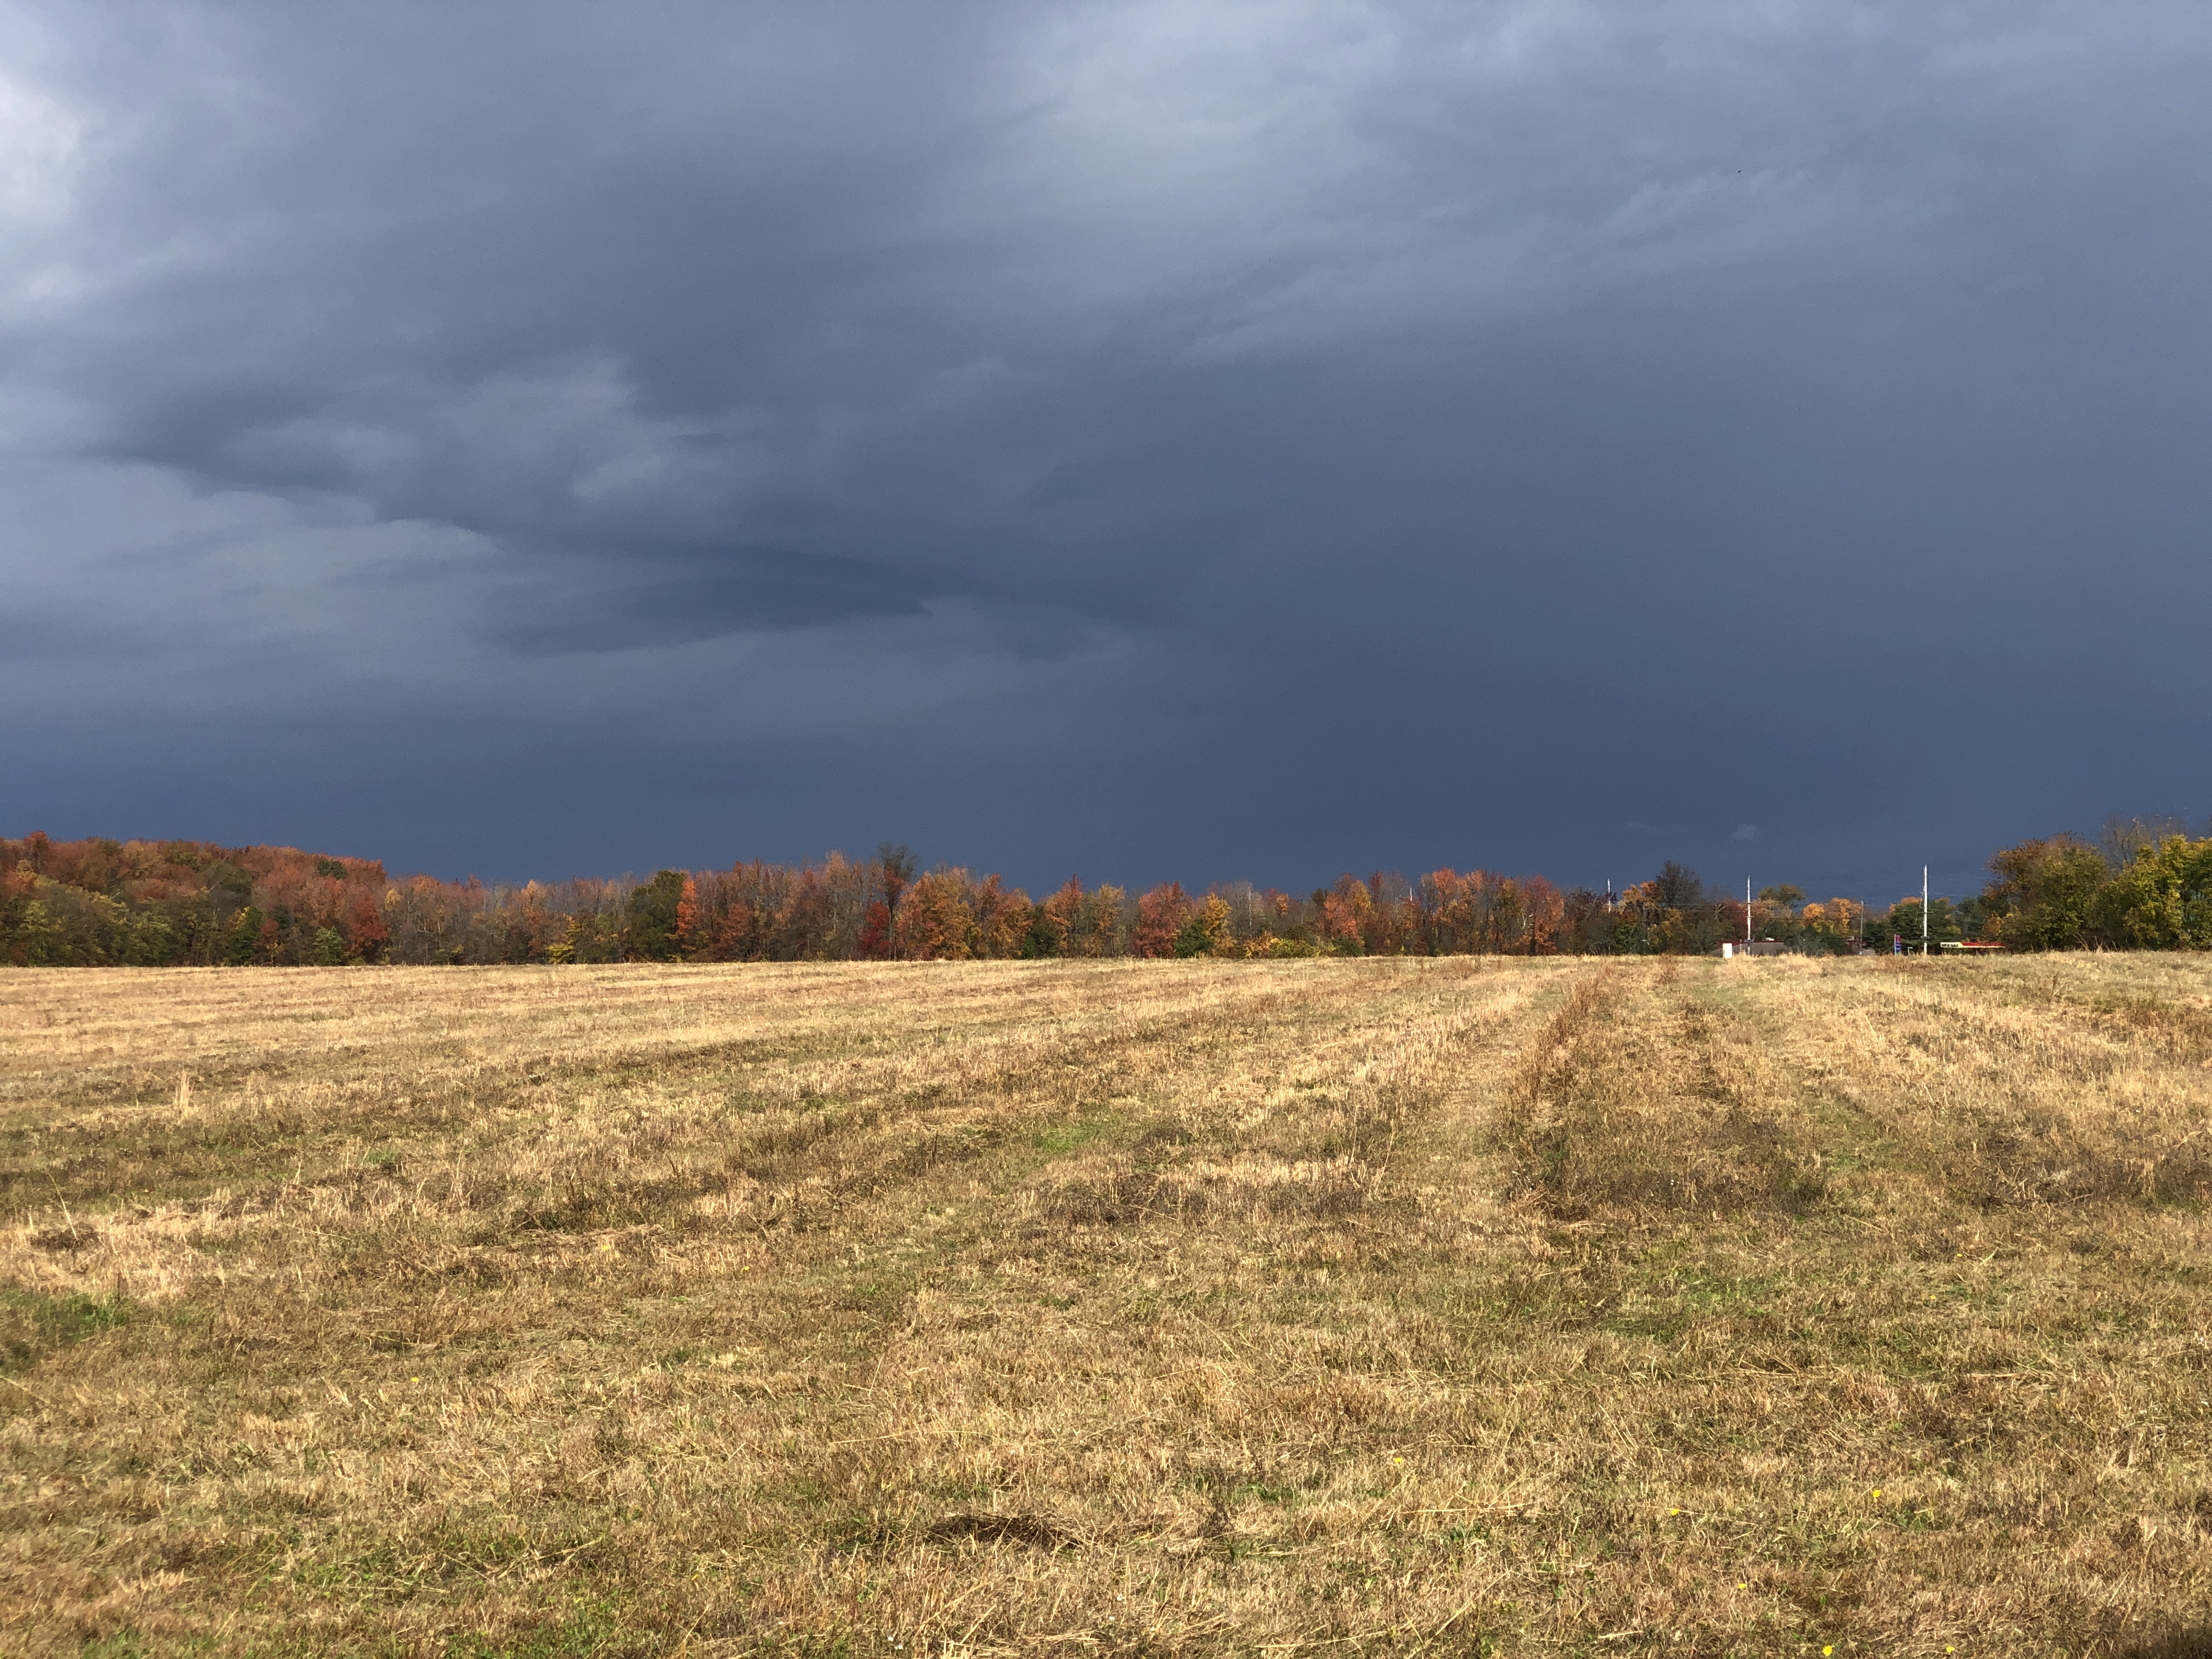
\includegraphics[width=\linewidth]{clouds/nimbostratus}
  \caption{Nimbostratus}
  \label{fig:nimbostratus}
  Источник\footnote{\url{https://commons.wikimedia.org/wiki/File:2023-10-29_12_25_34_View_towards_dark_clouds_from_Burlington_County_Route_630_(Woodlane_Road)_in_Westampton_Township,_Burlington_County,_New_Jersey.jpg}}
\end{figure}
  
\begin{figure}
  \centering
  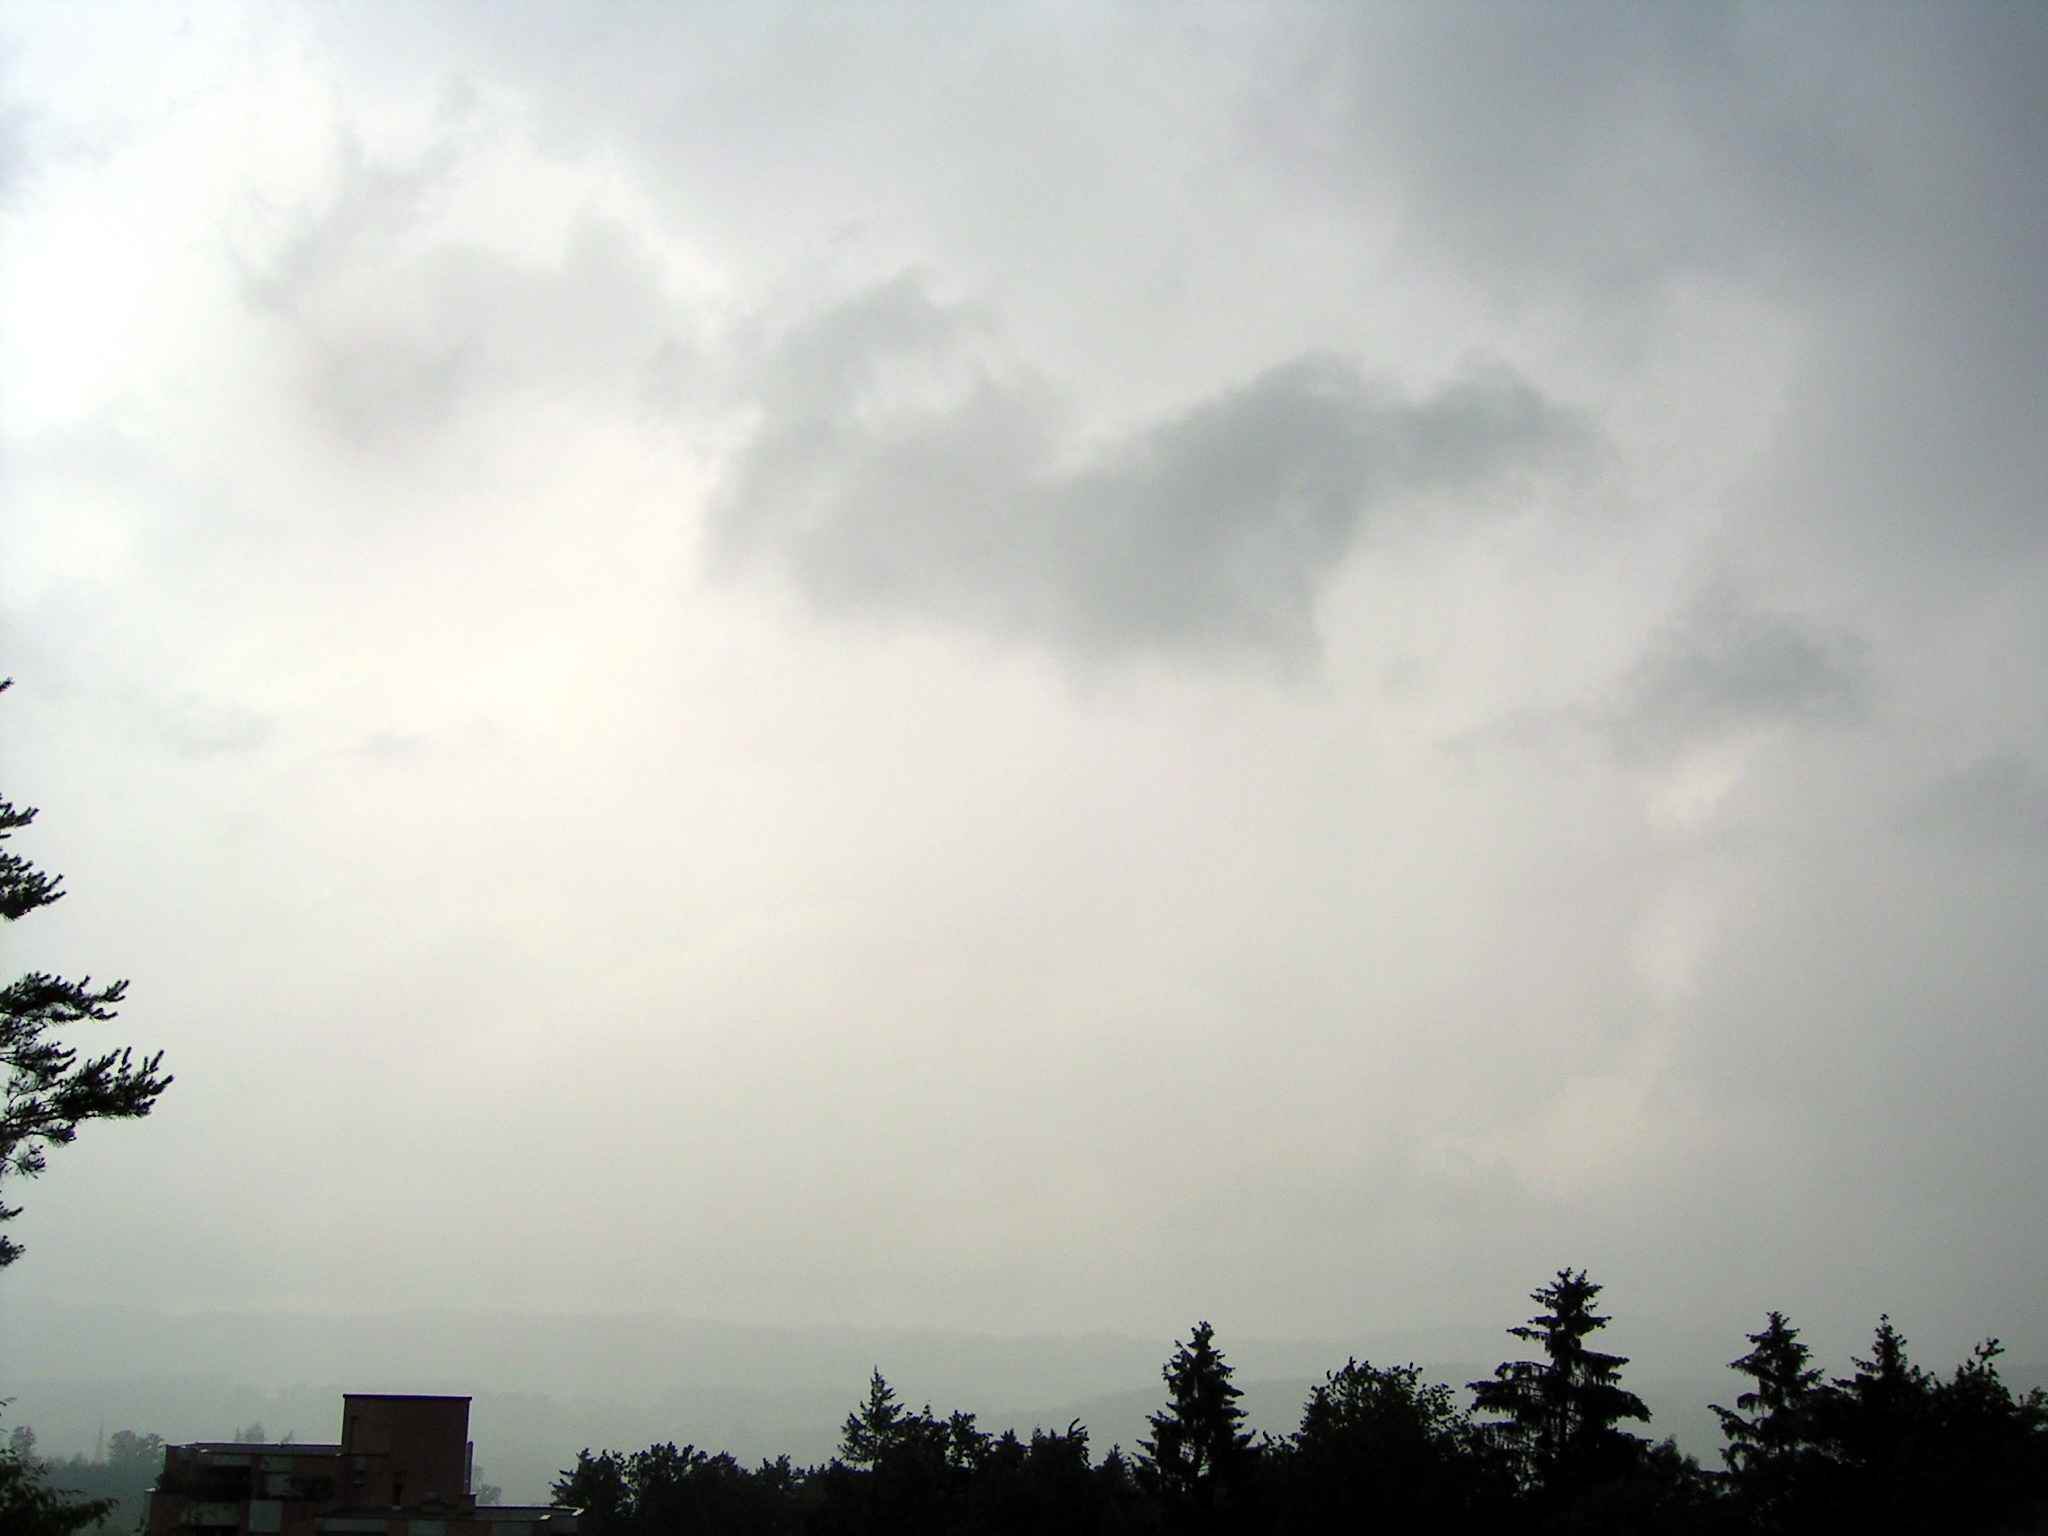
\includegraphics[width=\linewidth]{clouds/fractostratus_over_nimbostratus}
  \caption{Fractostratus на фоне Nimbostratus}
  \label{fig:fractostratus}
  Источник\footnote{\url{https://commons.wikimedia.org/wiki/File:Ns1.jpg}}
\end{figure}

\begin{figure}
  \centering
  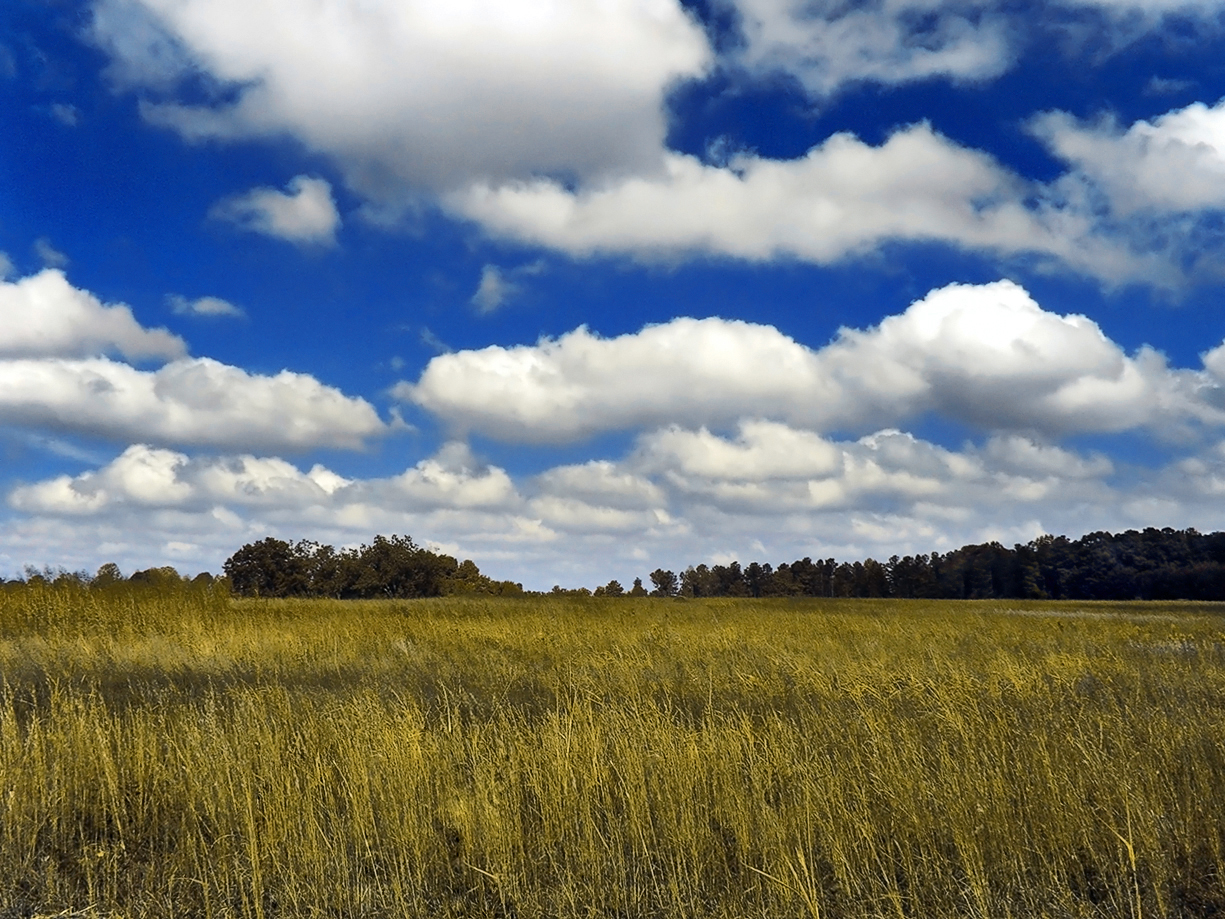
\includegraphics[width=\linewidth]{clouds/cumulus_humilis}
  \caption{Кучевые облака хорошей погоды, Cumulus humilis}
  \label{fig:112}
  Источник\footnote{\url{https://commons.wikimedia.org/wiki/File:Ns1.jpg}}
\end{figure}

\begin{figure}
  \centering
  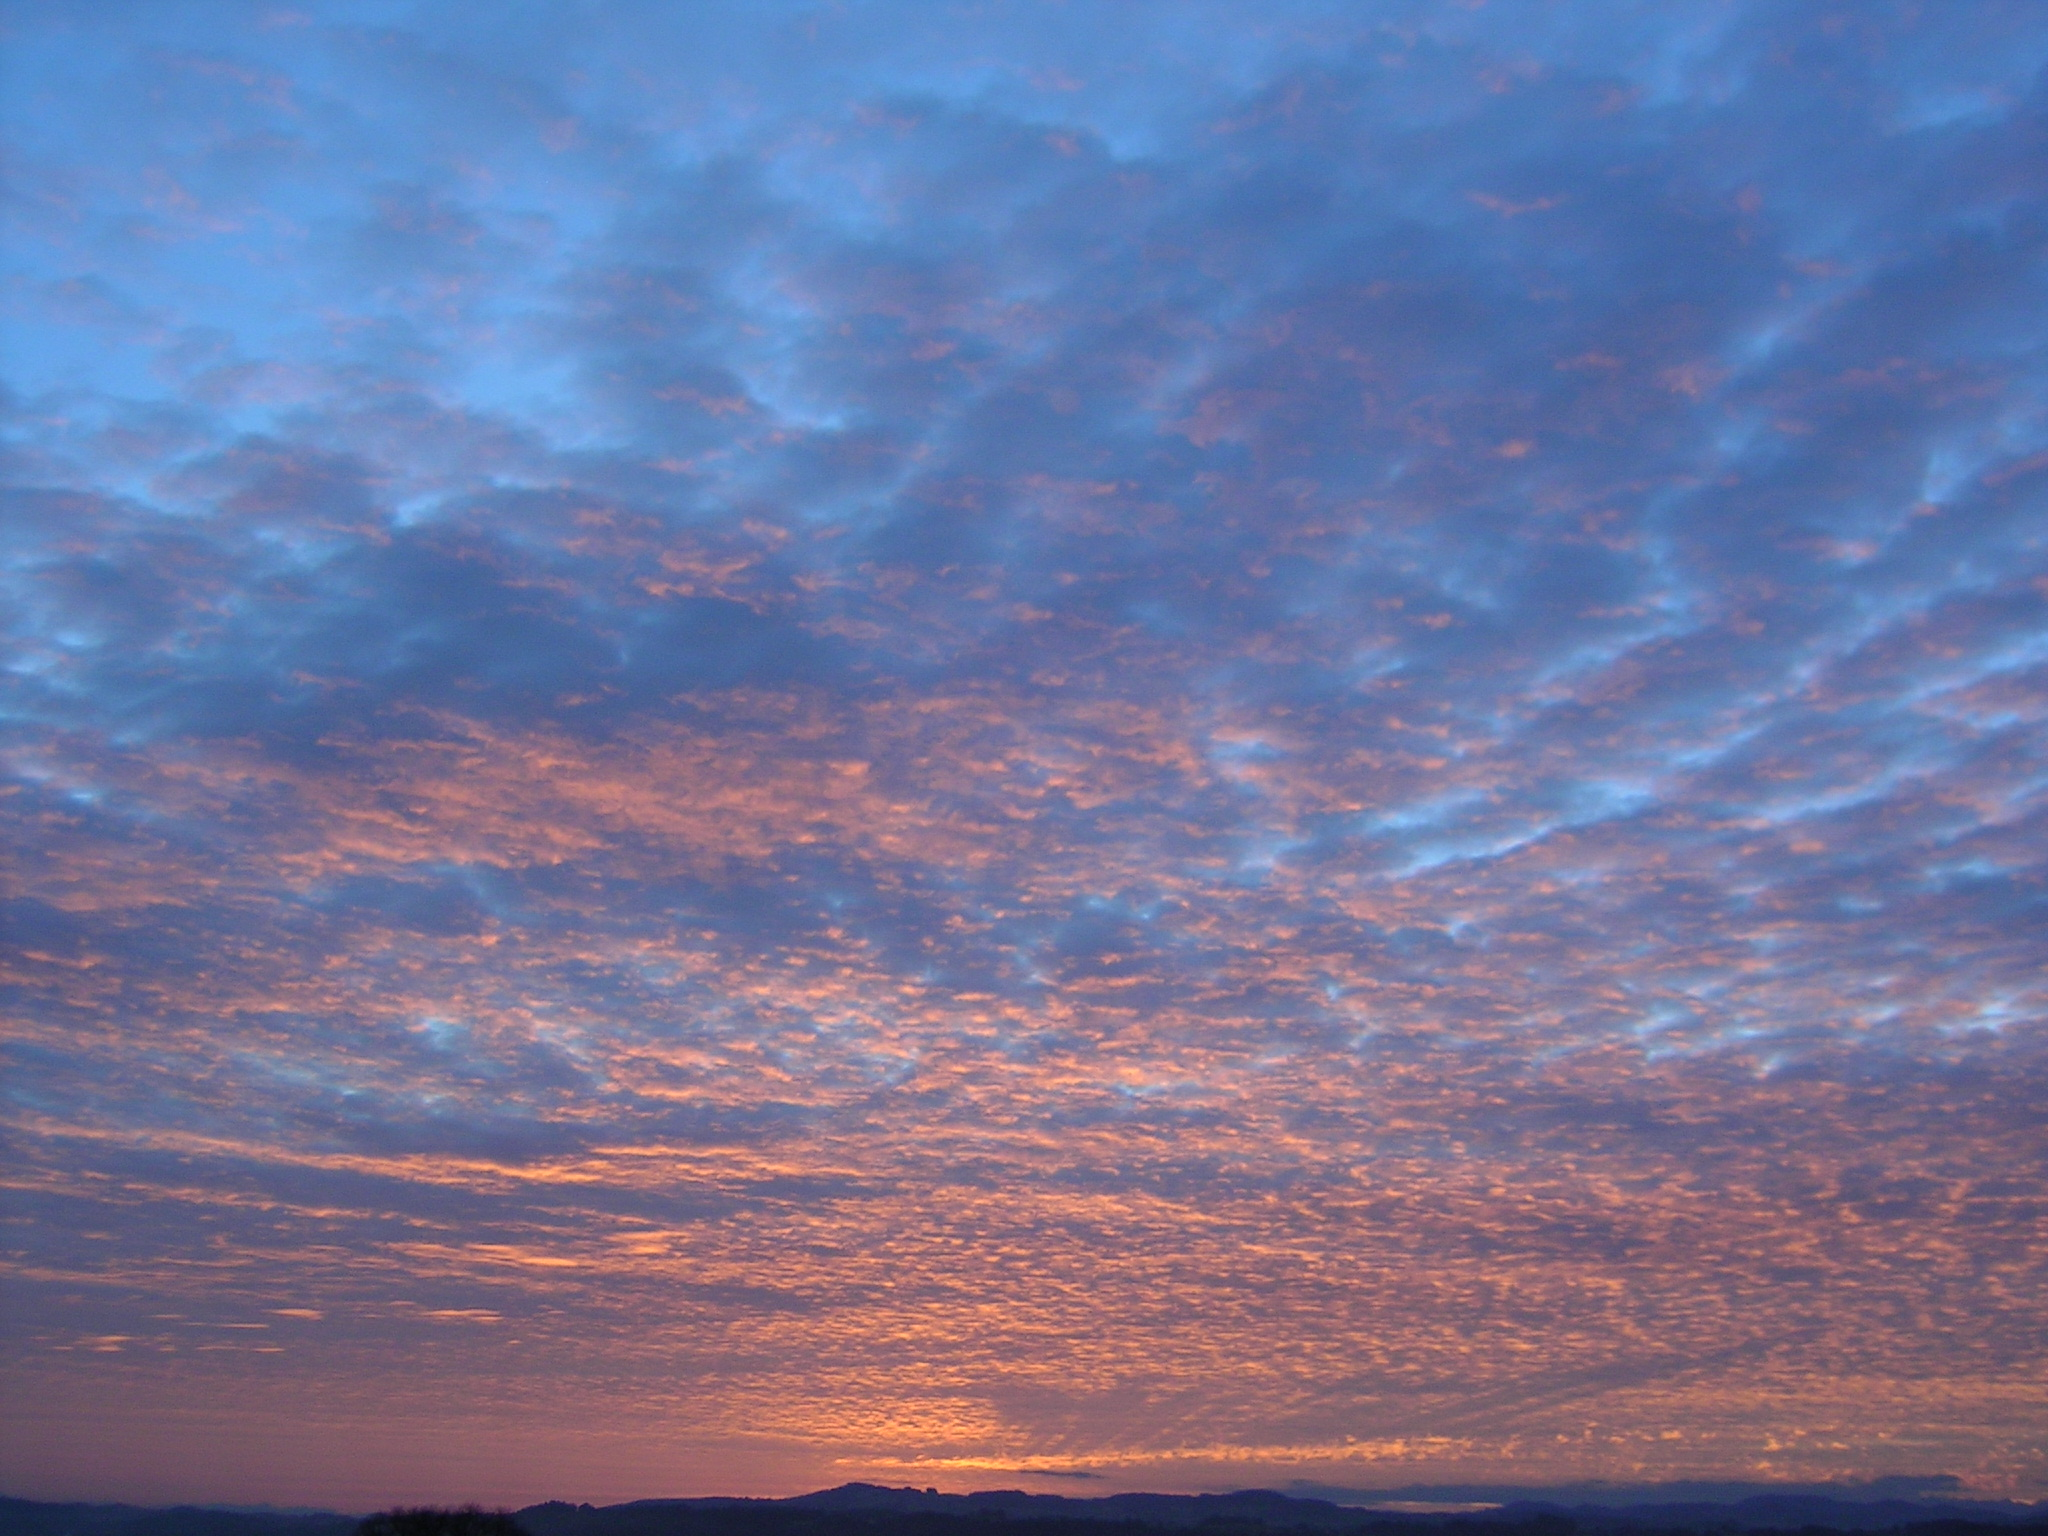
\includegraphics[width=\linewidth]{clouds/altocumulus}
  \caption{Высококучевые облака (<<барашки>>), Altocumulus}
  \label{fig:114}

\end{figure}

\begin{figure}
  \centering
  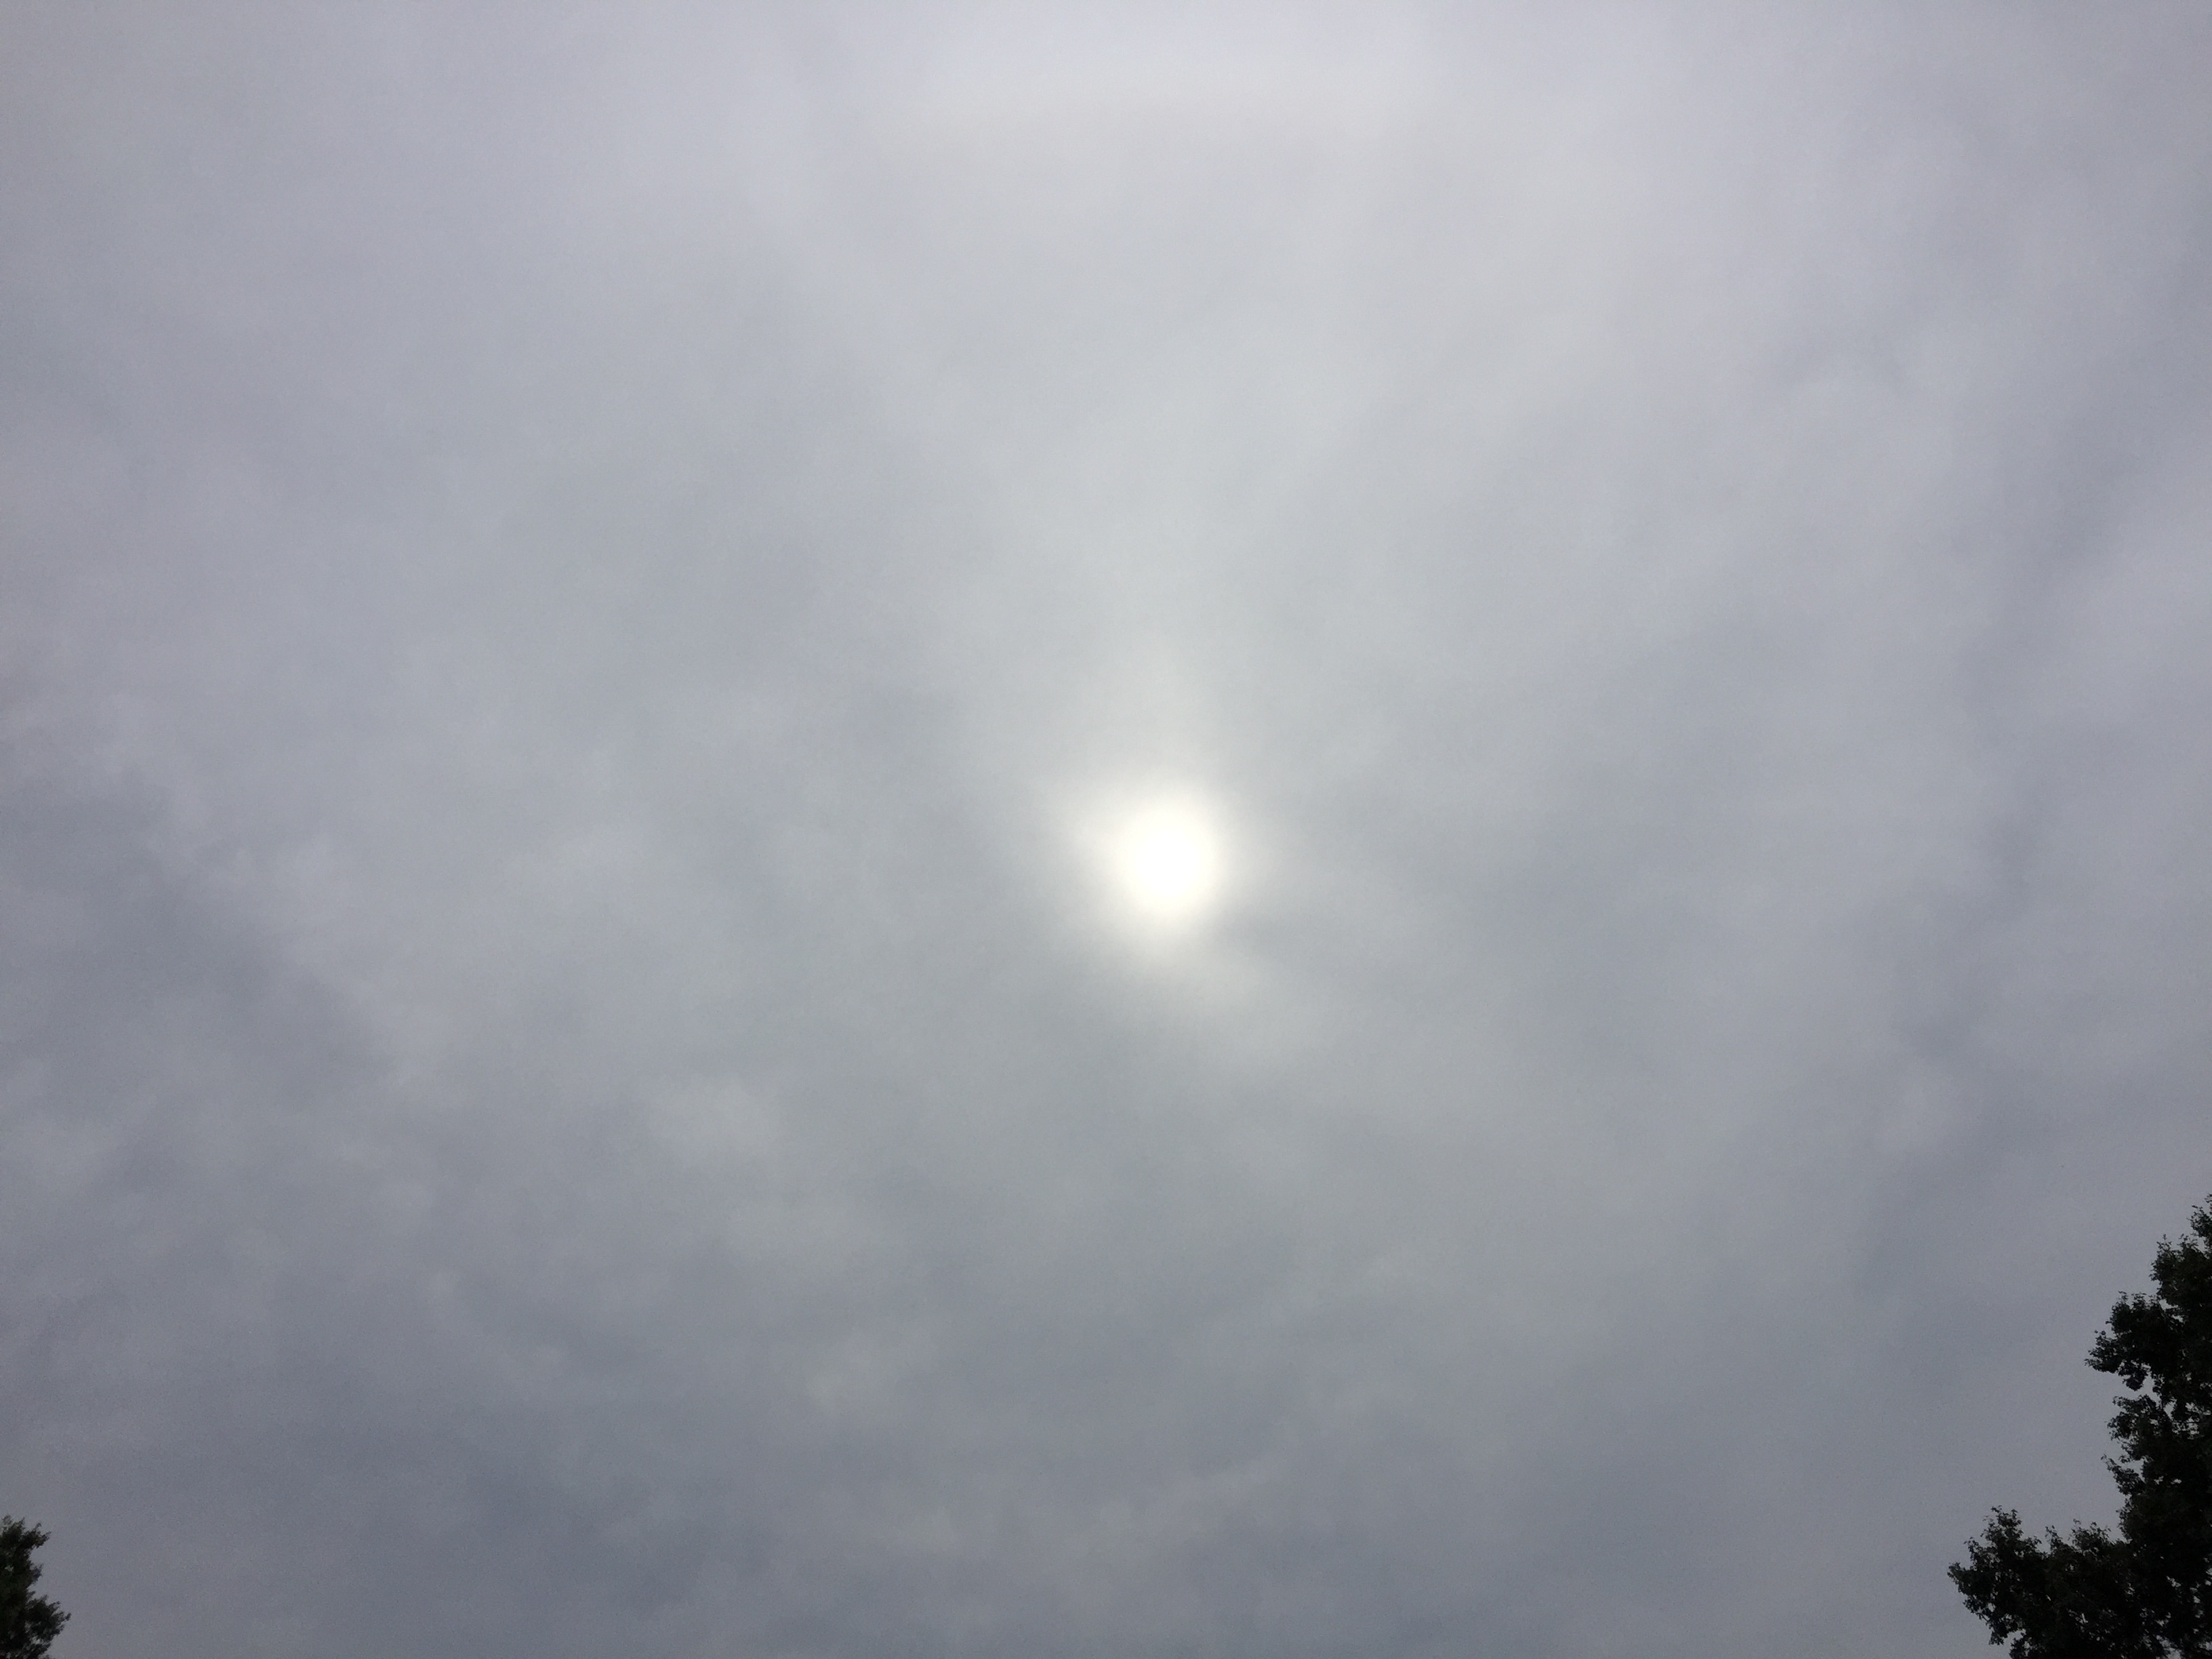
\includegraphics[width=\linewidth]{clouds/altostratus_translucidus}
  \caption{Солнце просвечивает через Altostratus translucidus}
  \label{fig:altostratus-translucidus}

\end{figure}

\begin{figure}
  \centering
  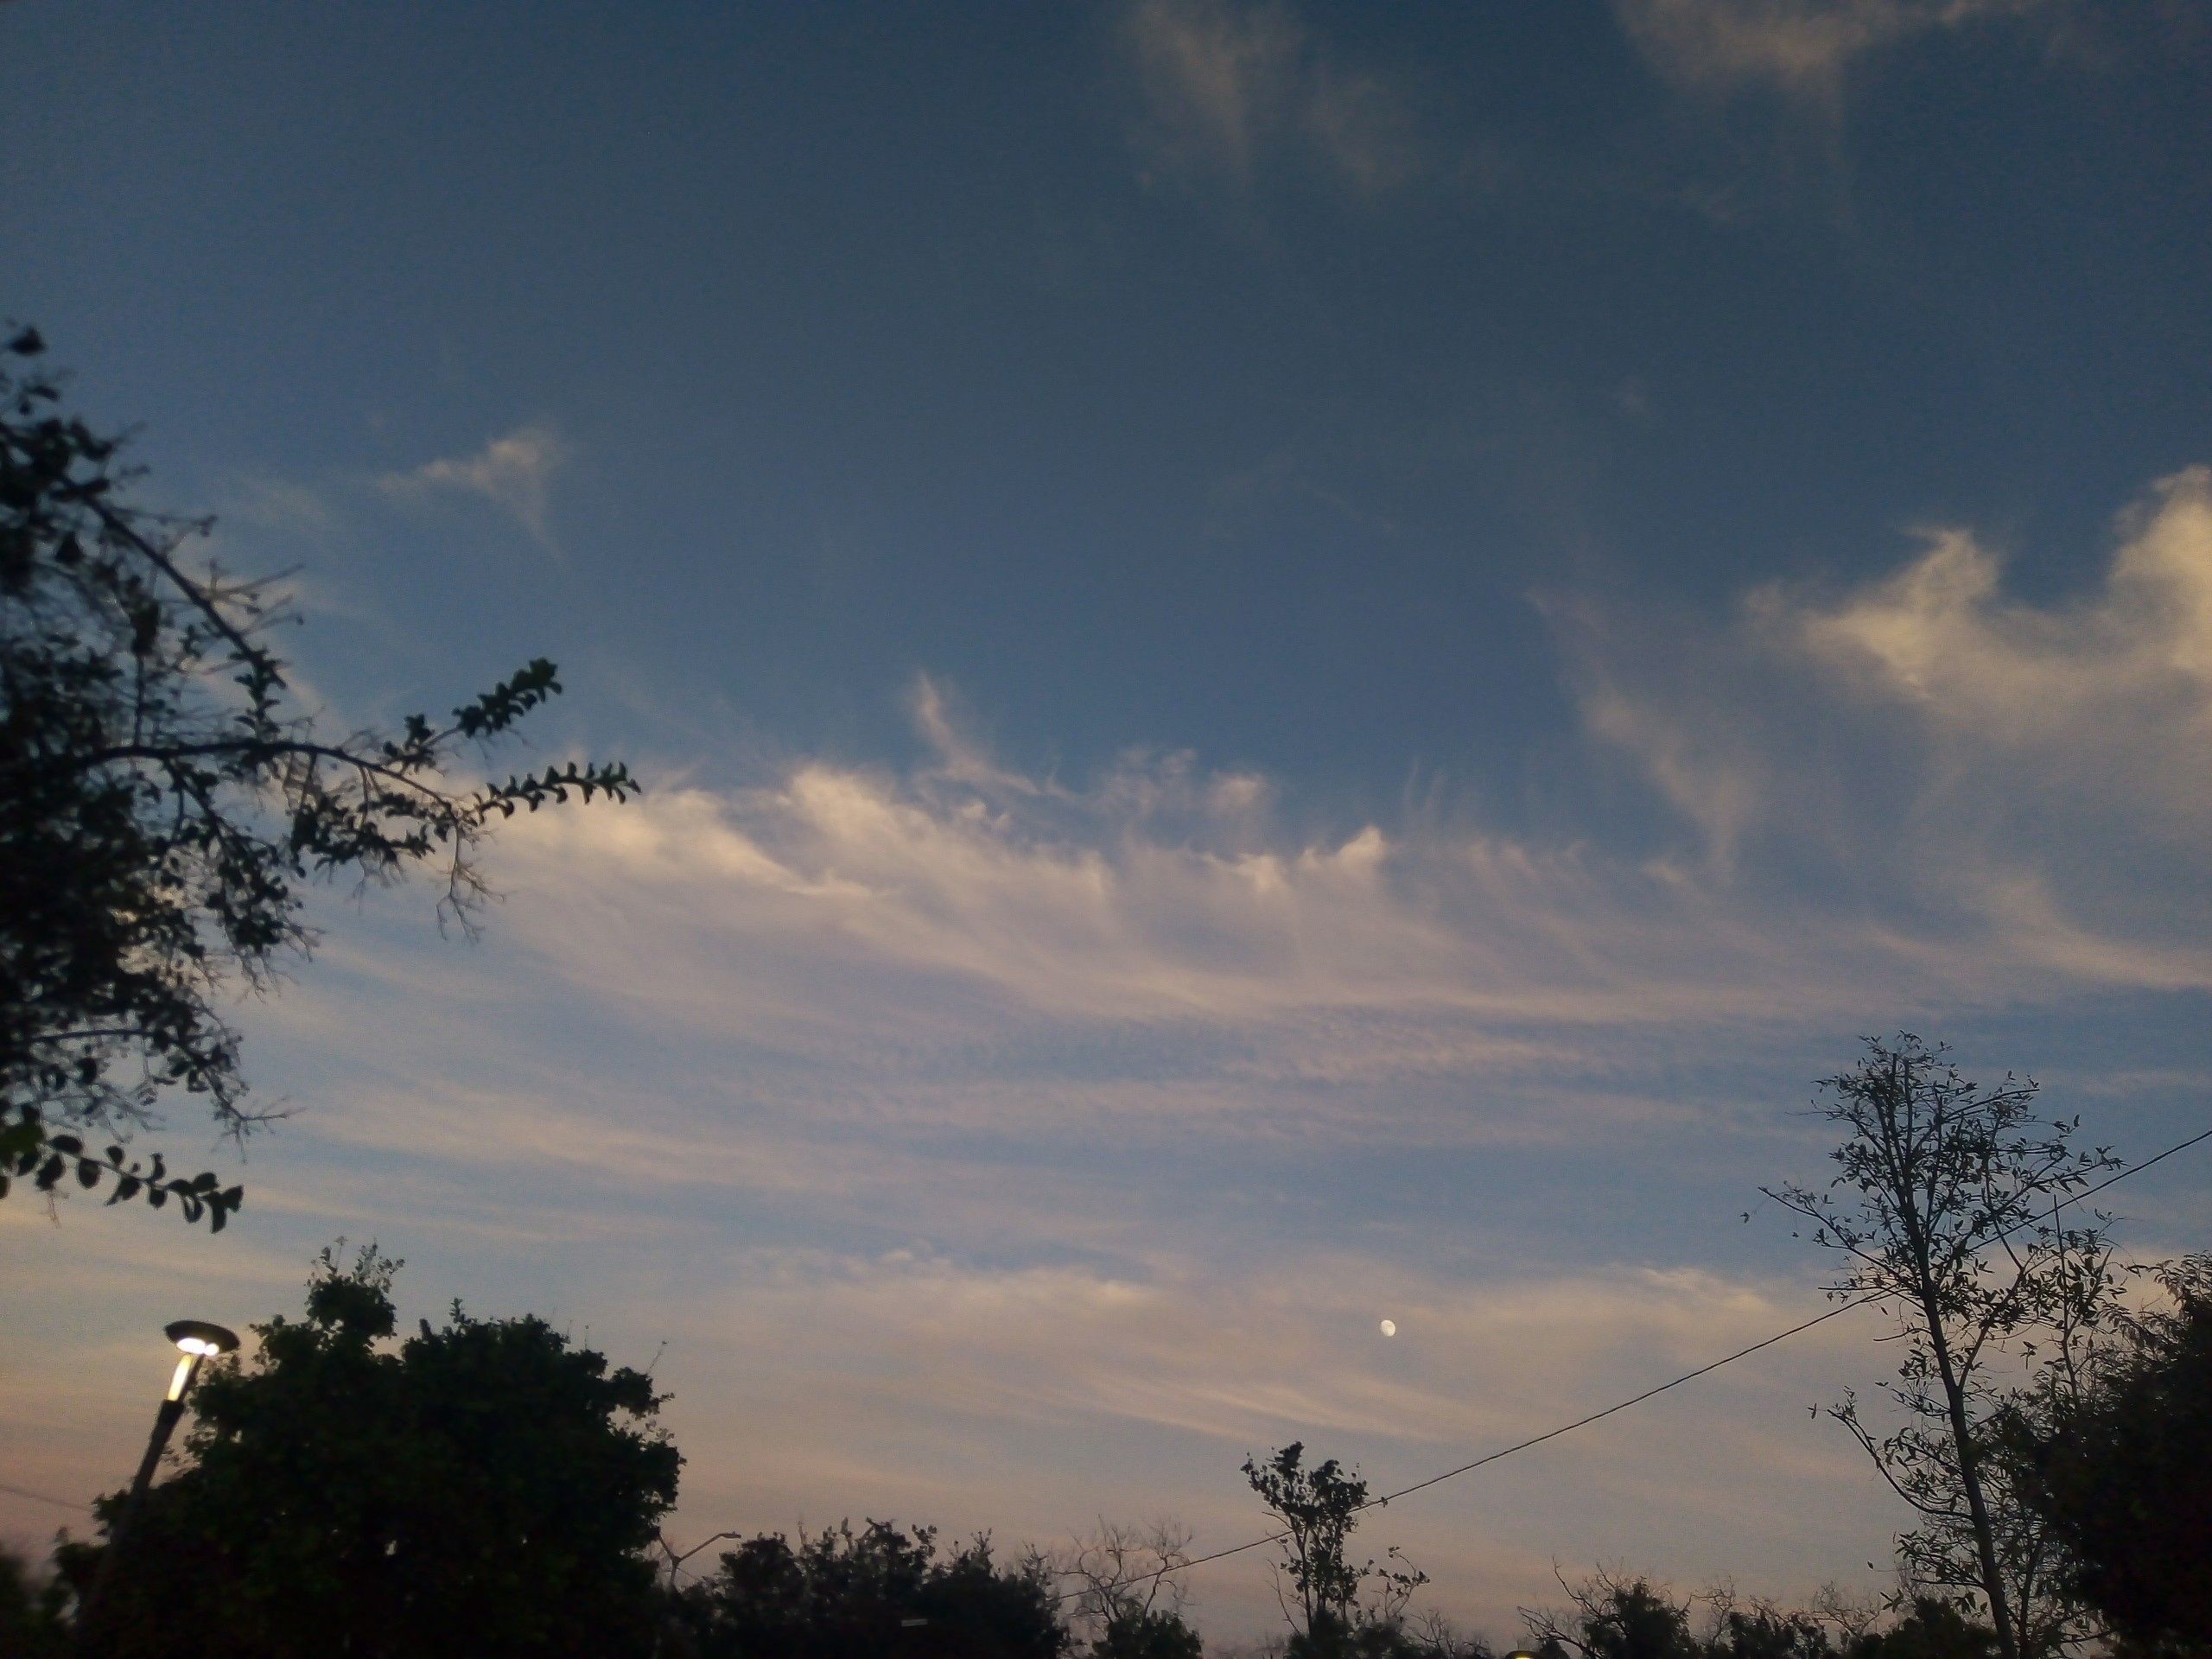
\includegraphics[width=\linewidth]{clouds/cirrus_floccus}
  \caption{Перистые облака, Cirrus flocus}
  \label{fig:115}

\end{figure}

\begin{figure}
  \centering
  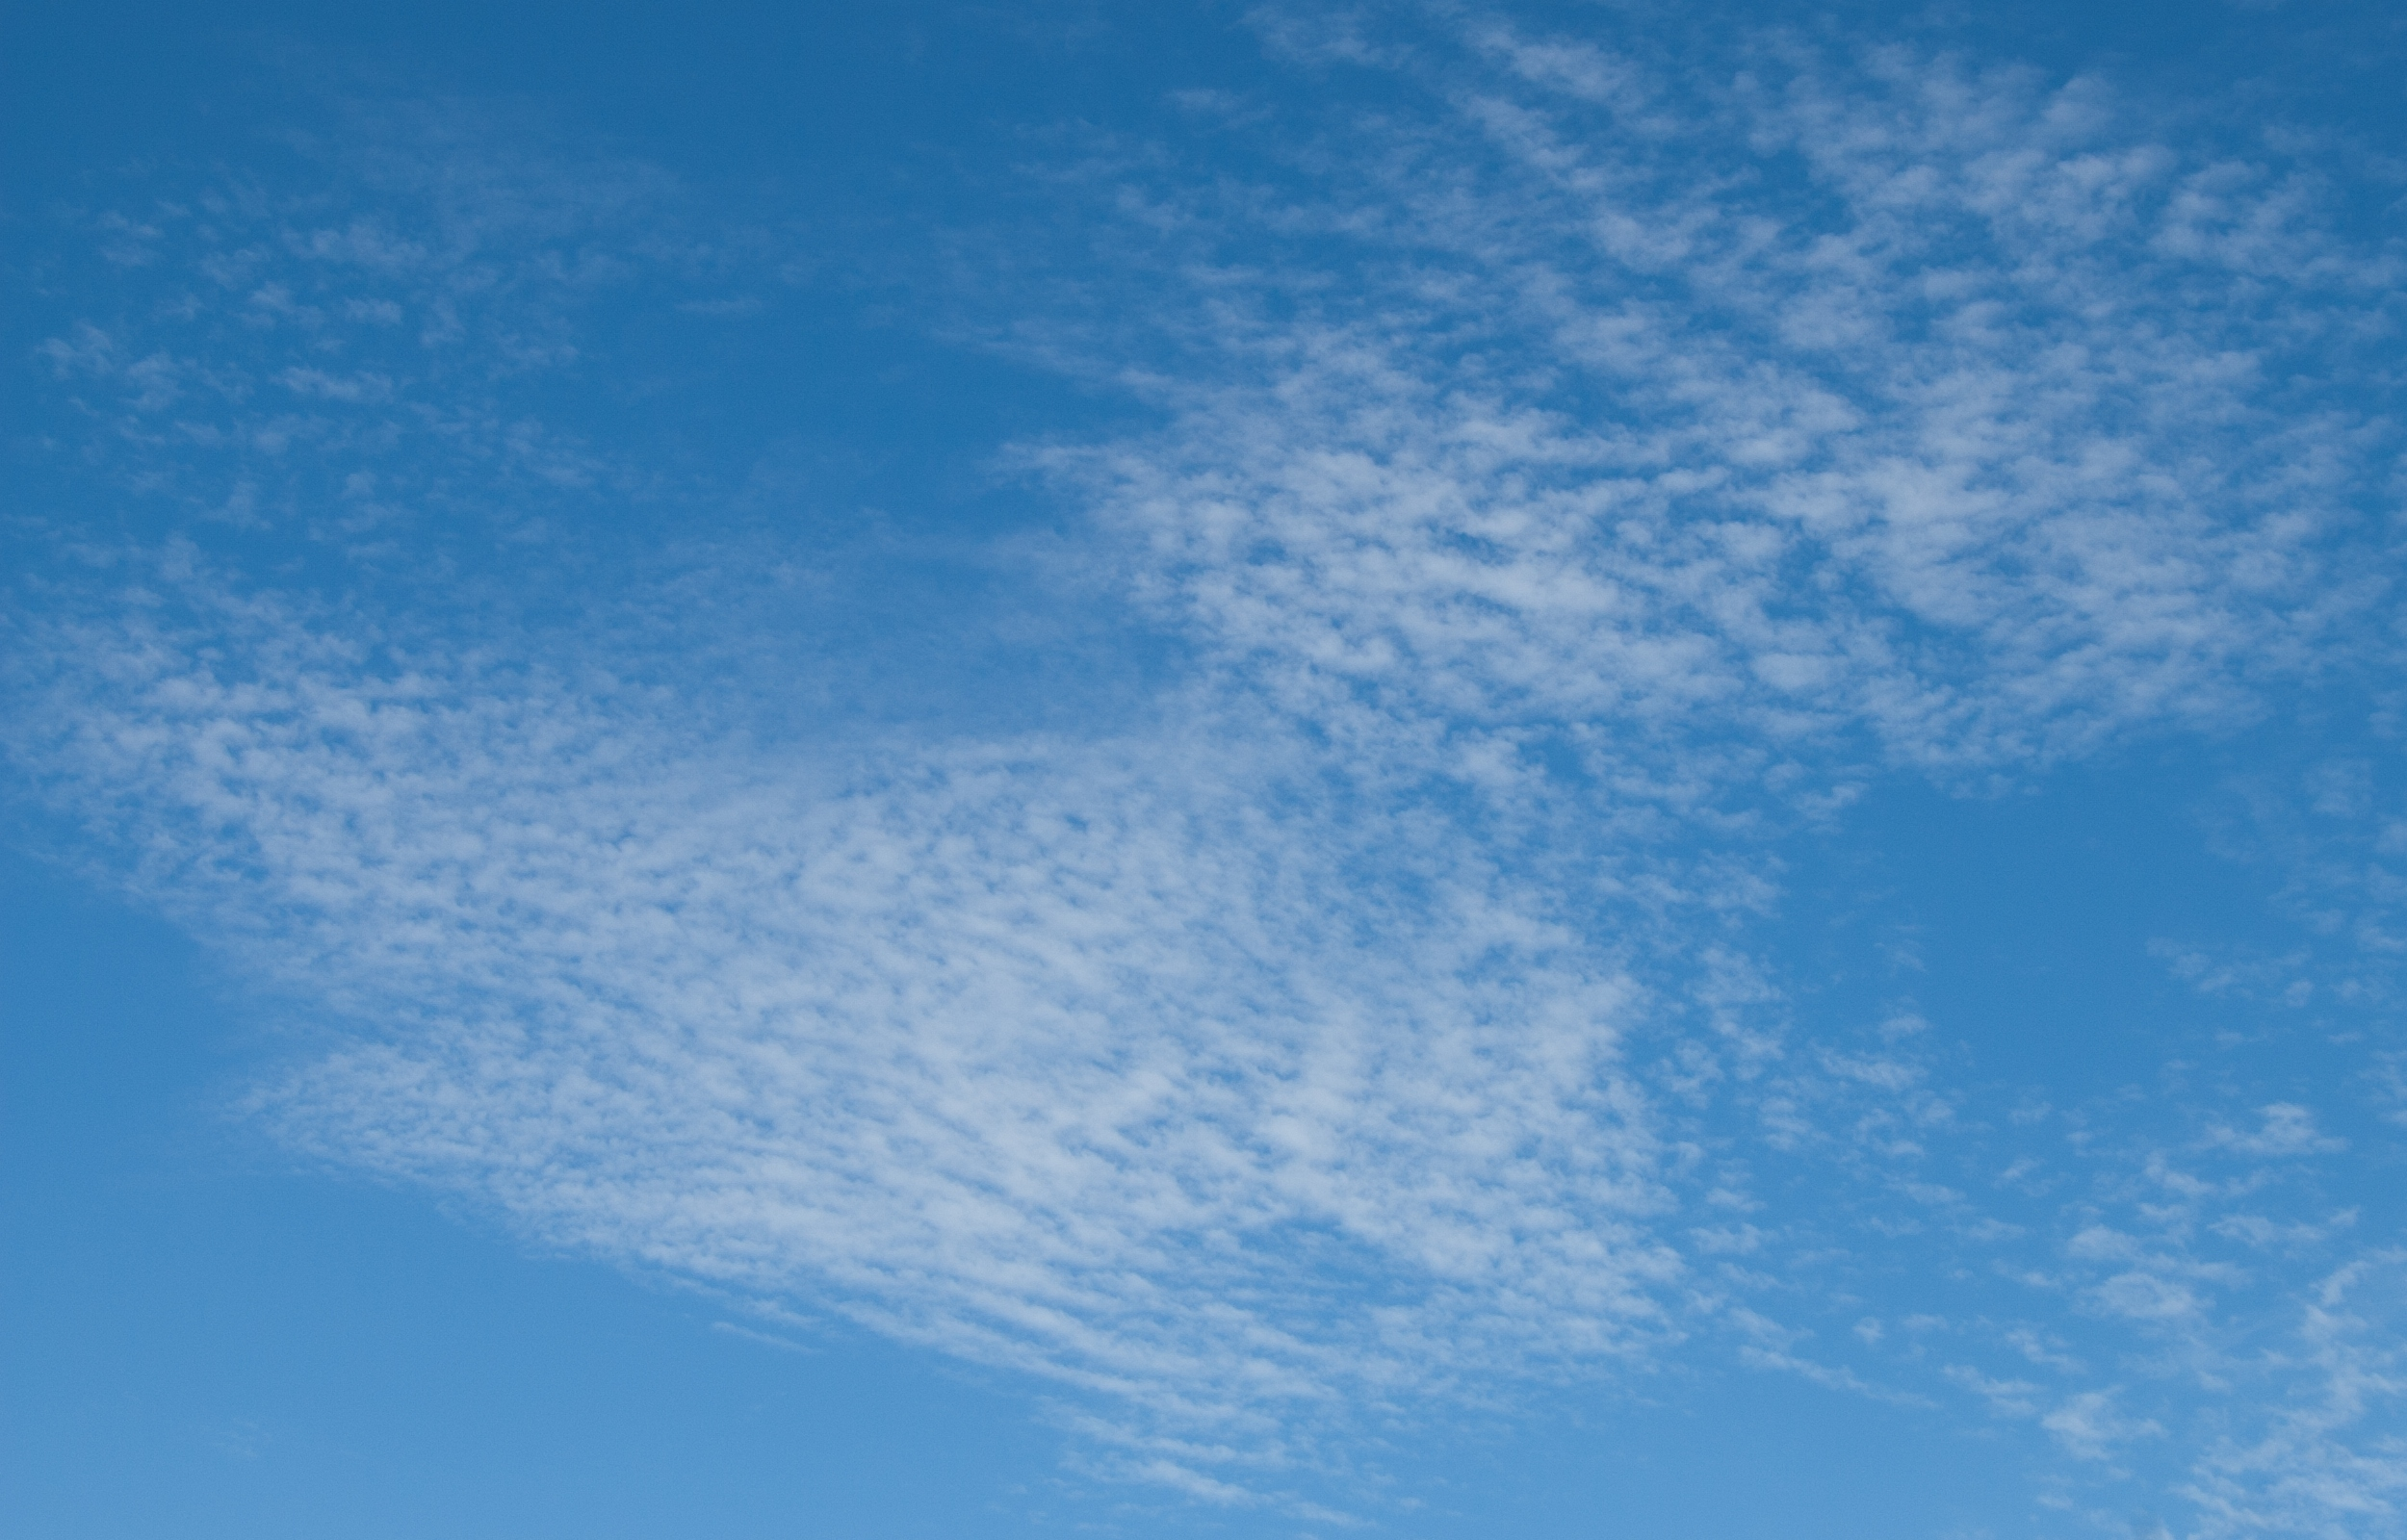
\includegraphics[width=\linewidth]{clouds/cirrocumulus}
  \caption{Перисто-кучевые, Cirrocumulus}
  \label{fig:cirrocumulus}

\end{figure}

\begin{figure}
  \centering
  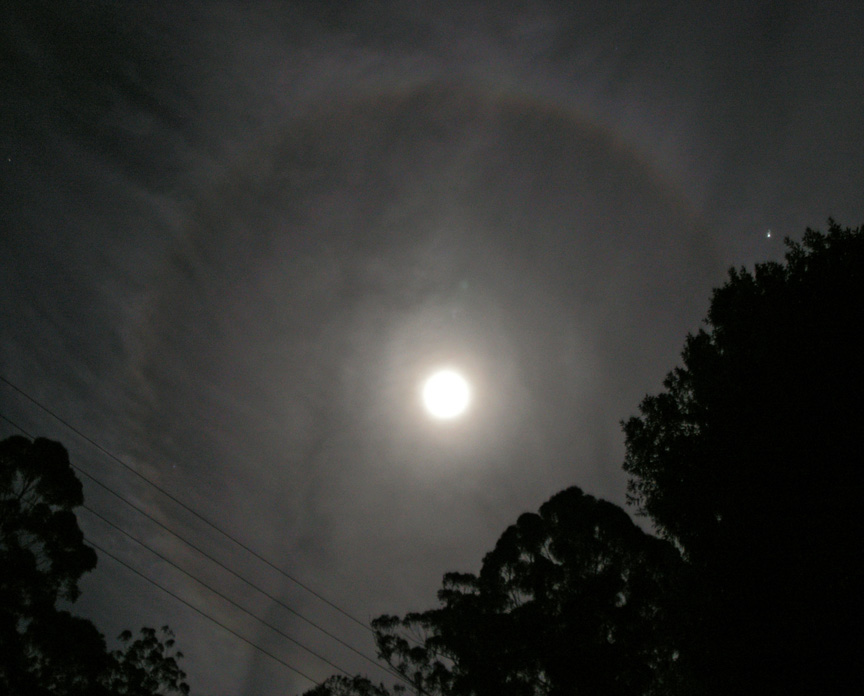
\includegraphics[width=\linewidth]{clouds/cirrostratus}
  \caption{Перисто-слоистые, Cirrostratus}
  \label{fig:cirrostratus}

\end{figure}

\begin{figure}
  \centering
  \includegraphics[width=\linewidth]{clouds/cumulonimbus}
  \caption{Кучево-дождевое облако (<<наковальня>>), Cumulonimbus calvus}
  \label{fig:113}

\end{figure}

\clearpage
}
\end{savenotes}

Классификация выглядит следующим образом:

\begin{enumerate}[label=\Roman*.]

\item Облака нижнего яруса.
  \begin{enumerate}[label=\arabic*)]
  \item Слоистые облака (стратус \--- \textit{St}) \--- высота
    0,05\otdo 0,5~км. Сплошной, однородный, серый, низконависающий
    покров. Обычно дают моросящие осадки. В отдельных случаях могут
    простираться до видимого горизонта (\rris{stratus}).
  \item Слоисто\-/кучевые (стратокумулюс \--- \textit{Sc}) \--- высота
    нижнего края 0,3\otdo 1,5~км. Сплошной волнистообразный серый
    покров, перемежающийся волнами и более светлыми промежутками между
    ними (\textit{Sc opacus}, \rris{stratocumulus-opacus}). Выше
    0,6~км образуются слоисто\-/кучевые просвечивающие облака
    (\textit{Sc translucidus}) серого цвета с просветами. Могут давать
    морось.
  \item Слоисто\-/дождевые (нимбостратус \--- \textit{Ns}) \--- высота
    0,1\otdo 1,0~км. Похожи на слоистые, но имеют более темный
    цвет (\rris{nimbostratus}). Сопровождаются обложными осадками.
  \item Разорванно\-/слоистые (фрактостратус \--- \textit{Fs}) \---
    сильно изорванные слоистые с просветами (\rris{fractostratus}).
  \end{enumerate}

\itemОблака вертикального развития.
  \begin{enumerate}[label=\arabic*)]
  \item Кучевые облака (кумулюс \--- \textit{Сu}) \--- высота от 0,3
    до 1,5~км. Белые кучи с серым плоским основанием и белыми
    кучеобразными вершинами. К ним относятся кучевые облака хорошей
    погоды (кумулехумилис \--- \textit{Сu hum}), разорванно\-/кучевые
    (фрактокумулюс \--- \textit{Fa сu}) и мощные кучевые (кумулюс
    конгестус \--- \textit{Сu cong}). Эти облака осадков не дают
    (рис.~\ris{112}).
  \item Кучево\-/дождевые (кумуленимбус \--- \textit{Сb}) \---
    вершинами достигают высоты перистых облаков (6\otdo 10~км),
    походят на горы или высокие башни. Тёмное основание лежит на
    высоте около 0,5~км. Вершины ярко\-/белые, состоят из ледяных
    кристалликов. Верхняя часть облака обычно размыта в стороны, имеет
    вид наковальни. Эти облака несут сильные ливневые осадки, грозы,
    град, сопровождаются шквалами\index{ветер!шквал}\index{шквал} (рис.~\ris{113}).
  \end{enumerate}

\item Облака среднего яруса.
  \begin{enumerate}[label=\arabic*)]
  \item Высококучевые (альтокумулюс \--- \textit{Ас}) \--- образуются
    на высоте 2\otdo 6~км, имеют вид светлых слоисто\-/кучевых
    просвечивающих облаков в сочетании с параллельными полосами
    пластинообразных и хлопьевых образований, параллельных гряд,
    осадков не дают (рис.~\ris{114}).
  \item Высокослоистые (альтостратус \--- \textit{As}) \--- образуются
    на высоте 3\otdo 5 км в виде пелены светло\-/серого или синеватого
    цвета. Могут быть просвечивающимися (\rris{altostratus-translucidus}) и плотные, создающие
    пасмурность.
  \end{enumerate}
  Все облака среднего яруса имеют смешанную структуру из смеси капелек с ледяными кристаллами. Осадки, выпадающие из них летом, поверхности земли не достигают.
  
\item Облака верхнего яруса. 
  \begin{enumerate}[label=\arabic*)]
  \item Перистые (циррус \--- \textit{Ci}) \--- лёгкие,
    волокнисто\-/нитевидной формы в виде белых отдельных волокон,
    иногда <<коготков>> (рис.~\ris{115}).
  \item Перисто\-/кучевые (циррокумулюс \--- \textit{Сс}) - мелкие
    <<барашки>>, иногда похожие на рыбью чешую (\rris{cirrocumulus}). Могут наблюдаться
    вместе с перистыми облаками.
  \item Перисто\-/слоистые (цирростратус \--- \textit{Cs}) \--- тонкая
    белесая прозрачная пелена, на фоне которой вокруг солнца или луны
    может образоваться ореол из цветных колец, так называемые круги
    гало (\rris{cirrostratus}). Эти и похожие явления \--- эффект преломления и отражения
    света в ледяных кристалликах, из которых и состоят перистые
    облака.
    \end{enumerate}
    Облака верхнего яруса находятся на высоте 6\otdo 10~км.
\end{enumerate}

Конденсат атмосферного водяного пара, выпадающий из облаков или
образующийся на поверхности земля и наземных предметах, называется
атмосферными \index{осадки!атмосферные} осадками, которые могут быть
жидкими (дождь, морось; на земле \--- роса) и твёрдыми (снег, снежная
крупа, град; на земле \--- иней, изморозь, гололёд).

По своему характеру выпадающие осадки могут быть:

\begin{description}
\item[ливневыми] \--- внезапными и быстротечными выпадениями дождя,
  снега, крупы или града из кучево\-/дождевых облаков обычно весной и
  летом;
\item[обложными] \--- продолжительный и равномерный дождь или снег,
  выпадающий из высокослоистых или слоисто\-/дождевых облаков при
  пасмурной погоде и на большой площади; в умеренных широтах
  преобладают осенью и зимой;
\item[моросящими] (морось) \--- мельчайшие капельки воды, не
  оставляющие следа на воде; выпадают из низких слоистых облаков или
  из густого тумана; чаще всего бывают осенью.
\end{description}

Скопление микроскопических капелек воды в нижних слоях атмосферы, при
которых горизонтальная видимость составляет менее полумили, называют
\textbf{туманом}\index{туман}. Образуются туманы при высокой относительной (около
100\,\%) влажности и в присутствии в воздухе ядер конденсации. По
причинам, их вызывающим, туманы делятся на:

\begin{description}
\item[радиационные] \--- возникающие над сушей в предутренние часы
  из-за потери тепла подстилающей поверхностью.  С повышением дневной
  температуры быстро рассеиваются. Для мореплавателя такие туманы,
  лежащие низко над землёй (позёмные), опасны тем, что, появляясь на
  побережье, могут закрывать плавучие и береговые знаки навигационного
  ограждения. При этом могут быть видимы высоко расположенные верхние
  части зданий, маяков, других береговых предметов. Над морем
  радиационные туманы появляются только в высоких широтах при большой
  относительной влажности воздуха;
\item[адвективные] (адвекция (лат.) \--- перенос), образующиеся на
  воде при перемещении тёплого влажного воздуха над охлаждённой
  поверхностью моря. Плотны и устойчивы к ветрам до
  10~м/с. Перемещаясь с ветром, они заволакивают большие
  районы. Видимость в адвективных туманах охлаждения может быть от
  нескольких десятков до нескольких метров. Имея большую высоту над
  уровнем моря, такой туман усложняет плавание, закрывая не только
  встречные суда, но и огни маяков;
\item[адвентивные туманы парения] \--- невысокие, до нескольких
  метров, клубящиеся туманы, возникающие при перемещении холодного
  воздуха над тёплой поверхностью моря. Встречаются при вторжении
  холодных масс арктического воздуха на незамерзающие моря в холодное
  время года.
\end{description}

Разновидностью тумана является туманная дымка, видимость при которой
0,5-5 миль.

Кроме осадков и туманов на ухудшение видимости может влиять
\textbf{сухая мгла}\index{сухая мгла} \--- механическое помутнение
атмосферы, которое встречается в море вблизи берегов при прохождении
мимо больших промышленных городов. Мгла состоит из дыма фабричных
труб, концентрации в воздухе различных неулавливаемых частиц пыли,
выхлопов двигателей автотранспорта, дыма лесных пожаров и
т.\=,д. Другой вид мглы образуется в результате сноса ветром с берега
(с сухих песчаных равнин и пустынь) в море пыли и мелкого песка. Смесь
тумана и мглы называют \textbf{смогом}\index{смог}.

В сухую жаркую погоду в море можно наблюдать явление оптической
мутности атмосферы, когда сильные конвективные токи воздуха различной
плотности перемешивают его. При этом в неоднородной воздушной среде
при разных температуре и давлении резко меняются условия отражения,
рассеивания и преломления световых лучей: предметы теряют свою
чёткость, становятся расплывчатыми искажённым, снижая тем условия
видимости.

\begin{table*}[htb]
  \centering
  \begin{tabular}{l|p{0.2\textwidth}|p{0.3\textwidth}|c}
    \toprule
    Дальность видимости & Характеристика видимости & Условия видимости & Баллы \\
    \midrule
    До 1/4 каб. & \multirow{3}{*}{Очень плохая} & Очень сильный туман & 0 \\
    До 1 каб.   & & Сильный туман & 1 \\
    До 2\otdo 3 каб. & & Умеренный туман & 2 \\
    \midrule
    Около 0,5 мили & \multirow{2}{*}{Плохая} & Слабый туман & 3 \\
    От 0,5 до 1 мили & & Очень сильный дождь, умеренная дымка или мгла & 4 \\
    \midrule
    1\otdo 2 мили & \multirow{2}{*}{Средняя} & Сильный дождь, слабая дымка или мгла & 5 \\
    1\otdo 5 миль & & Умеренный дождь & 6 \\
    \midrule
    5\otdo 11 миль & Хорошая & Слабый дождь & 7 \\ 
    \midrule
    11\otdo 27 миль & Очень хорошая & Без осадков & 8 \\ 
    \midrule
    выше 27 миль & Отличная & Совершенно чистый воздух & 9 \\
    \bottomrule
  \end{tabular}  
  \caption{Шкала метеорологической видимости (для летнего плавания)}
  \label{tab:5}
\end{table*}

В отличие от навигационной метеорологическая видимость определяется
предельным расстоянием видимости наблюдаемого предмета в условиях
данной погоды. Для определения дневной дальности метеорологической
видимости существует десятибалльная шкала (табл.~\ref{tab:5}).

\section{Ветер. Общая циркуляция атмосферы}

Перемещение масс воздуха из области высокого атмосферного давления в
область с низким давлением называется
\textbf{ветром}\index{ветер}. Скорость ветра определяется величиной
барического градиента, т.\=,е. разностью атмосферного давления на
установленную единицу расстояния, равную 60 милям (1\gr широты), в
сторону падения давления. Поэтому скорость ветра тем больше, чем
больше барический градиент. Величину и направление барического
градиента на карте изобар показывают в виде вектора перпендикулярного
изобаре большего давления, направленного в сторону меньшего
давления. Вследствие вращения Земли (под влиянием силы Кориолиса)
направление ветра не совпадает с вектором барического градиента, а
отклоняется в северном полушарии вправо, в южном \--- влево. В средних
широтах это отклонение достигает 60\gr.

\begin{figure}[!htb]
  \centering{}
  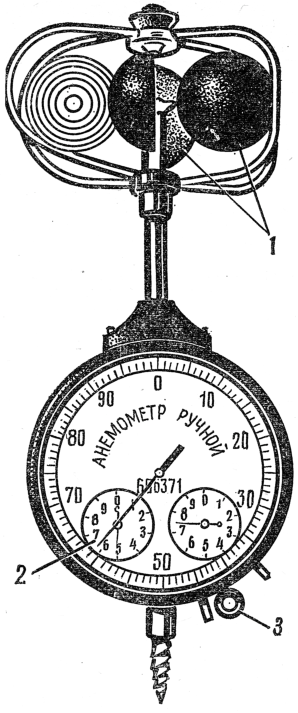
\includegraphics[scale=1.2]{0116P}
  \caption{Ручной анемометр}
  \label{fig:116}
  \small
  \centering{}
  \textit{1} \--- полушария крестовины; \textit{2} \--- отсчёт 6175; \textit{3} \--- стопор (арретир)
\end{figure}

На отклонение ветра влияет также кривизна самих изобар, вызывающая
криволинейное движение воздуха под действием центробежной силы,
направленной по радиусу кривизны. В циклоне\index{циклон} центробежная сила
направлена против силы градиента, а в антициклоне\index{антициклон} совпадает с
ней. Поэтому при одинаковом градиенте скорость ветра в циклоне всегда
меньше, чем в антициклоне.

По традиции направление ветра считается из той точки горизонта, откуда
он дует. Иначе говоря, ветер дует в компас, направление обозначается в
румбах\footnote{в настоящее время синоним направления} (иногда в
градусах). Также в компас принято определять направление зыби, а из
компаса, в направлении на горизонт, морские течения.

Единицами измерения скорости ветра являются <<метр в секунду>>,
<<километр в час>>, <<узел>>. Практически же скорость ветра с помощью
анемометра измеряется в м/с или приближённо оценивается <<сила ветра>>
по шкале Бофорта (табл.~\ref{tab:6}).

Для измерения скорости ветра в судовых условиях применяется
\textit{ручной анемометр}\index{анемометр} (рис.~\ris{116}). Ветер,
вращая крестовину с четырьмя полыми полушариями, приводит в движение
счётчик прибора, который через три стрелки даёт показания на
циферблат. Точное значение скорости ветра надо узнать из таблицы
поправок в аттестате анемометра.

При порывистом ветре определяют его среднюю скорость \--- по
нескольким сделанным подряд измерениям и находят среднее
арифметическое значение. Другой способ: проводят наблюдение в течение
нескольких минут, а затем делят полученную разность отсчётов на
соответствующее число секунд.

Ветер по своей структуре не однороден. Он может быть струйным
(ламинарным), когда слои воздуха движутся не перемешиваясь, их частицы
не переходят из слоя в слой. Такое движение воздуха обычно бывает при
слабых ветрах. Если же скорость ветра превышает 4~м/с, то частицы
воздуха начинают двигаться беспорядочно, его слои перемешиваются и
приобретают турбулентный характер. Чем выше скорость ветра, тем больше
турбулентность, тем больше скачки скорости в отдельных точках
воздушного потока и тем более порывистым становится
ветер. Табл.~\ref{tab:7} показывает, как меняется ветер в зависимости
от его скорости и направления.

Шквалистый ветер характерен не только частыми и резкими колебаниями
скорости, но и сильнейшими отдельными порывами продолжительностью до
нескольких минут. Ветер, который резко увеличивает свою скорость в
течение очень короткого промежутка времени на фоне слабого ветра или
штиля, называют шквалом\index{ветер!шквал}\index{шквал}. Чаще всего
шквалы налетают при прохождении мощных кучево\-/дождевых облаков и
нередко сопровождаются грозой и ливнями. Скорость шквального ветра
достигает 20~м/с и более, а в отдельных порывах \--- 30\otdo
40~м/с. При этом наблюдаются неожиданные повороты ветра до нескольких
румбов. Основной причиной шквала является взаимодействие восходящего
потока тёплого воздуха в передней части кучево-дождевого облака и
нисходящего воздуха, охлаждённого ливневым дождём, в тыловой его
части.В результате возникает характерный клубящийся вал с вихрем под
ним, усиленным вихрями соседних воздушных слоев (см. рис.~\ris{136}).

Вертикальные вихри в грозовом облаке могут образовать
\textit{смерчи}\index{смерч}\index{ветер!смерч}. Когда скорость такого
вихря достигает около 100~м/с, нижняя часть облака в виде воронки
опускается к воде, навстречу поднимающемуся вверх водяному
столбу. Встреча со смерчем опасна: обладая большой разрушительной
силой и вращаясь по спирали, он может поднять вверх все, что окажется
на его пути. Высота смерча достигает более 1000~м, горизонтальная
скорость \-- 30\otdo 40~км/ч. Поэтому при виде смерча нужно определить
направление его перемещения и немедленно уходить в сторону.

Иногда смерч может образоваться и без грозовых облаков. В этом случае
он зарождается не из тучи, а на поверхности моря, нередко при
безоблачном небе. Это \textit{смерчи <<хорошей погоды>>}\index{ветер!смерч!хорошей погоды}.
Они быстро разрушаются и практически безопасны.

\begin{table*}
  \centering{}
  \begin{tabular}{l|c|c|c}
    \toprule
    \multirow{2}{*}{\shortstack{Характеристика\\ветра}} & \multirow{2}{*}{\shortstack{Время\\наблюдения\\(мин.)}} & \multicolumn{2}{c}{Пределы отклонений} \\
    \cmidrule{3-4}
    & & \shortstack{по\\направлению} & \shortstack{по\\скорости} \\
    & & & \\
    \midrule
    \textbf{По направлению:} & & & \\
    постоянный & 2\otdo 5 & 1 румб & - \\
    меняющийся & >> & \shortstack{Более 1 румба} & - \\
    \midrule
    \textbf{По скорости:} & & & \\
    ровный & 2\otdo 5 & - & Не более 4 м/с \\
    порывистый & >> & - & Более 4 м/с \\
    шквалистый\index{ветер!шквал}\index{шквал} & >> & - & Более 10 м/с \\
    \bottomrule
  \end{tabular}
  \caption{Характеристики изменения ветра}
  \label{tab:7}
\end{table*}

\begin{figure}[!htb]
  \centering{}
  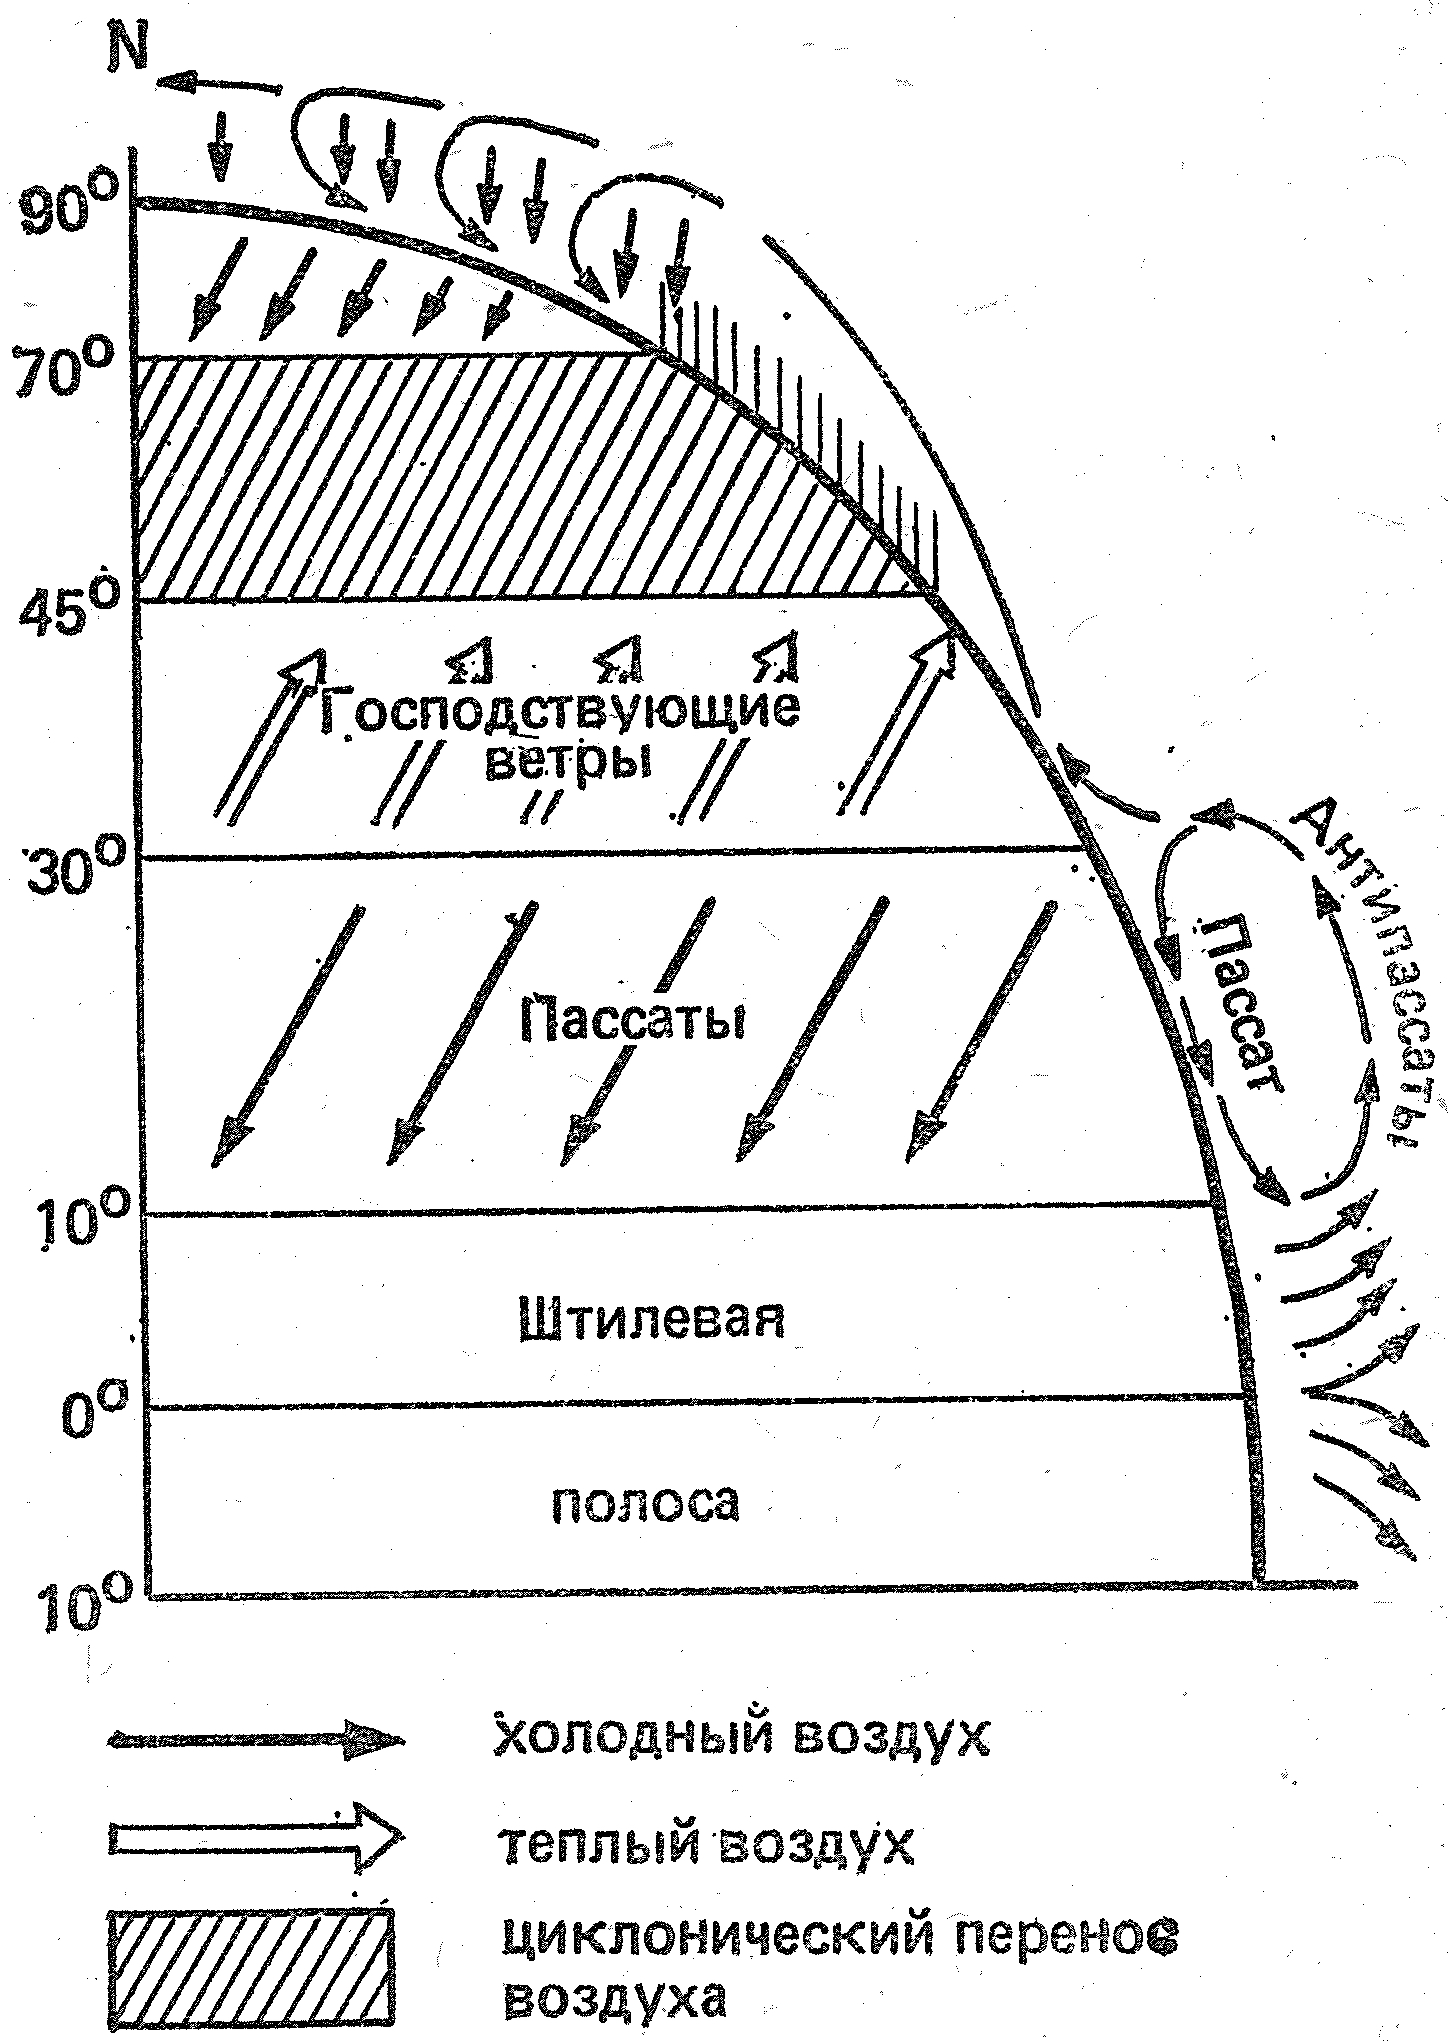
\includegraphics[width=\linewidth]{0117P}
  \caption{Схема общей циркуляции атмосферы}
  \label{fig:117}
\end{figure}

Как мы уже говорили, движение воздушных масс величина переменная и по
скорости, и по направлению. Однако в масштабах глобальных это движение
имеет чётко выраженную закономерность, которая определяется общей
циркуляцией атмосферы, зависящей от распределения атмосферного
давления в обширных районах земного шара \--- от тропиков до Полярных
зон. На схеме циркуляции воздуха между земной поверхностью и верхними
слоями атмосферы (рис.~\ris{117}) видно, как вертикальные и
горизонтальные потоки воздушных масс превращаются в ветры, имеющие
постоянный сезонный характер.

В экваториальной зоне тёплый воздух тропиков поднимается вверх, на
границе тропосферы образуя ветер антипассат, растекающийся к северу и
к югу.

Охлаждённые воздушные массы
\textbf{антипассата}\index{антипассат}\index{ветер!антипассат} оседают
на поверхность земли, создавая в субтропиках повышенное давление и
ветер, называемый уже
\textbf{пассатом}\index{пассат}\index{ветер!пассат}, который
устремляется в экваториальную зону.

Под действием силы Кориолиса\index{сила!Кориолиса} пассаты северного полушария получают
северо\-/восточное направление, а южного полушария (кроме северной
части Индийского океана, где дуют сезонные муссонные ветры) \---
юго\-/восточное. Скорость пассатных ветров также постоянна и достигает
5\otdo 10~м/с.

В экваториальной зоне пассаты ослабевают и поворачивают на
восток. Поэтому между пассатами обоих полушарий возникает штилевая
зона (в Атлантике \--- \textit{<<конские широты>>}\index{конские широты}),
характерная пониженным давлением, грозами, ливнями и штилями.

В широтах 40\otdo 60\gr обоих полушарий преобладают ветры западной
четверти. Они менее устойчивы (от $NW$ до $SW$), но значительно
сильнее (10\otdo 15~м/с или 6\otdo 7 баллов). В южном полушарии, где
западные ветры огибают весь Мировой океан, лежали основные пути
парусных судов для плавания из Европы в Австралию и обратно в Европу
вокруг мыса Доброй Надежды и мыса Горн. За свою силу и частые штормы
(повторяемость до 50\,\%) эти ветры получили прозвище <<бравые
весты>>\index{бравые весты}, а широты \---
<<гремящие сороковые>>\index{гремящие сороковые} и
<<ревущие шестидесятые>>\index{ревущие шестидесятые}.

В приполярных районах обоих полушарий, где оседают холодные массы
воздуха верхних слоев тропосферы (при вертикальном температурном
градиенте, падающем на 0,6\grC на каждые 110~м высоты.), образуя так
называемые полярные максимумы, преобладают юго\-/восточные и восточные
ветры.

Пассаты\index{ветер!пассат} \--- первые в категории
\textbf{господствующих ветров}\index{ветер!господствующий},
т.\=,е. постоянно дующих в определённых районах течение определённого
промежутка времени. Скорость и направление господствующих ветров
определяется многолетним наблюдениям для каждого моря или морского
района.

Другая категория ветров \--- \textbf{местные}\index{ветер!местный},
дующие только в данном месте или нескольких местах земного шара
возникают они при изменении тепловых условий в течение некоторое
времени или под влиянием рельефа местности (характера подстилающей
поверхности).

\begin{figure}[!htb]
  \centering{}
  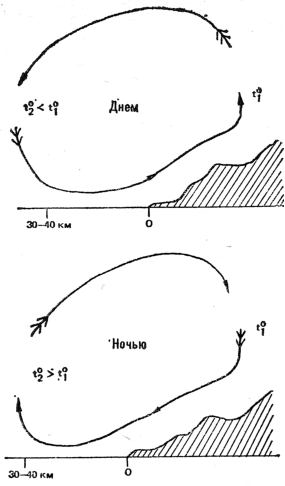
\includegraphics[width=\linewidth]{0118P}
  \caption{Бризы}
  \label{fig:118}
\end{figure}

К первому типу относятся следующие ветры:
\begin{description}
\item [Бриз]\index{бриз} \--- ветер, возникающий из неравномерного нагревания воды
  суши в прибрежной полосе моря (около 30\otdo 40~км). Морской бриз
  дует днем с моря на сушу и начинает около 10 часов утра, а береговой
  \--- суши на море и начинается после захода солнца. Ветер
  вертикально развития и на высоте нескольких с метров дует в обратном
  направлении (рис.~\ris{118}). Интенсивность бриза зависит от
  погоды. В жаркие летние дни морской бриз имеет умеренную силу до 4
  баллов (4\otdo 7~м/с). Береговой бриз значительно слабее;
\item[Фен]\index{фен} \--- горячий сухой ветер, который возникает при обтекании
  влажно воздуха ветром горных вершин и нагревании его тёплой
  подветренной подстилающей поверхностью горного склона. На Чёрном
  море наблюдает у побережья Крыма и Кавказа преимущественно весной.
\end{description}

Представителем второго типа местных ветров надо назвать прежде всего
бору:
\begin{description}
\item[Бора]\index{бора} \--- очень сильный, порывистый и холодный
  ветер, направленный вниз по горному склону в местностях, где горный
  хребет граничит с тёплым морем. Холодный воздух с большой скоростью
  устремляется вниз, к морю, достигая иногда силы урагана. В зимнее
  время, при низких температурах, вызывает обледенение. Наблюдается в
  районе Новороссийска, у берегов Далмации (Адриатическое море) и на
  Новой Земле;
\item[Бакинский норд]\index{бакинский норд} \--- холодный северный
  ветер в зоне Баку, дующий летом и зимой. Достигает штормовой, а
  нередко и ураганной силы (от 20 до 40~м/с). Приносит с берега тучи
  песка и пыли;
\item[Сирокко]\index{сирокко} \--- очень тёплый и влажный ветер,
  зарождающийся в Африке и дующий в Центральной части Средиземного
  моря. Сопровождается облачностью и осадками.
\end{description}

Все сведения о господствующих\index{ветер!господствующий} и
местных\index{ветер!местный} ветрах для данного моря (или
морского района) даются в Лоциях.

\begin{figure}[!htb]
  \centering{}
  \includegraphics[width=\linewidth]{0119P}
  \caption{Муссоны}
  \label{fig:119}
\end{figure}

Существуют также сезонные ветры, называемые муссонами, которые носят
континентальный характер и возникают вследствие разницы в атмосферном
давлении при неравномерном нагревании суши и моря в летнее и зимнее
время.

Как и другие ветры, муссоны имеют барический градиент\index{барический градиент}, направленный в
сторону низкого давления \--- летом на сушу, зимой на море
(рис.~\ris{119}). Под влиянием силы Кориолиса в северном полушарии
летние муссоны Тихого океана у восточного побережья Азии отклоняются к
юго\-/востоку, а в Индийском океане \--- к юго\-/западу. Эти муссоны
приносят с океана на Дальний Восток пасмурную, с дождями, моросью и
туманами погоду, а на южное побережье Азии несут затяжные и обильные
дожди, частые наводнения.

Зимние муссоны меняют направление на противоположное (120\gr\otdo
180\gr), и в Тихом океане они дуют уже с северо\-/запада, а в
Индийском \--- с северо\-/востока в сторону океана. Скорость ветра в
муссонах неравномерна. Зимние северо\-/восточные муссоны совпадают с
пассатами\index{ветер!пассат} северного полушария, и их скорость не превышает 5\otdo
10~м/с. Летние же муссоны Индийского океана достигают штормов
силы. Смена муссонов происходит в апреле\--мае и октябре\--ноябре.

\begin{figure}[!htb]
  \centering{}
  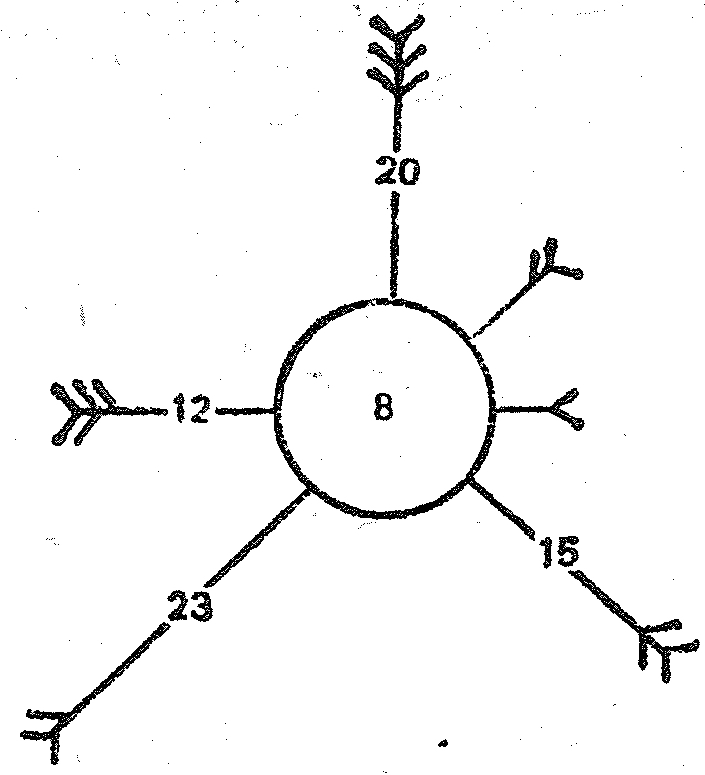
\includegraphics[width=\linewidth]{0120P}
  \caption{Роза ветров}
  \label{fig:120}
\end{figure}

Ветер \--- основной движитель парусного судна. Поэтому с его
направлением и силой приходится считаться в первую очередь. При выборе
наиболее благоприятного маршрута для длительного крейсерского плавания
полезно воспользоваться картой ветров, на которой поверхность моря или
океана разбита на квадраты. В центре квадрата, внутри кружка, цифрами
указывается повторяемость штилей. От центра кружка расходятся лучи по
главным и четвертным румбам. Длина лучей пропорциональна повторяемости
ветров этого направления, а на их концах наносится оперение,
показывающее среднюю силу ветра. Если повторяемость ветра более
12\,\%, то на луче пишется величина повторяемости, если меньше 5\,\%
\--- лучей не делают. Этот графический способ нанесения на карту
ветровой обстановки на определённое время года, исчисленной на
основании многолетних наблюдений, называется
\textbf{розой ветров}\index{роза ветров} (рис.~\ris{120}).

Изучая розы ветров, лежащие на пути яхты, капитан может оценить
ветровую обстановку при проработке маршрута плавания.

  \onecolumn
  {\small
  \begin{longtable}{c|c|c|p{0.2\textwidth}|p{0.2\textwidth}|c}
    \toprule
    \multirow{6}{*}{\begin{sideways}\shortstack{Баллы\\Бофорта}\end{sideways}} &
    \multirow{6}{*}{\begin{sideways}\shortstack{Характеристика\\ветра}\end{sideways}} &
    \multirow{6}{*}{\begin{sideways}\shortstack{Скорость ветра\\м/с (интервал)}\end{sideways}} &
    \multicolumn{2}{c|}{Действие ветра} &
    \multirow{6}{*}{\begin{sideways}\shortstack{Давление\\$H/\text{м}^2$}\end{sideways}} \\
    \cmidrule{4-5}
    &\ &\ & \centering{} \multirow{3}{*}{\shortstack{на судне}} & \centering{} \multirow{3}{*}{\shortstack{на море}} & \\
    &\ &\ &\ &\ & \\
    &\ &\ &\ &\ & \\
    &\ &\ &\ &\ & \\
    &\ &\ &\ &\ & \\
    \midrule
    1 & 2 & 3 & \centering{} 4 & \centering{} 5 & 6 \\
    \midrule
    \endfirsthead
    \toprule
    1 & 2 & 3 & \centering{} 4 & \centering{} 5 & 6 \\
    \midrule
    \endhead
    \shortstack{0\\(0)} & Штиль & 0\otdo 0,2 & Дым поднимается вертикально. Вымпел неподвижен & Зеркально-гладкая поверхность & 0 \\
    \midrule
    \shortstack{1\\(1)} & Тихий	& \shortstack{1\\(0,3\otdo 0,5)} & По дыму можно определить направление ветра & Рябь. Пены на гребнях нет & 0,1 \\
    \midrule
    \shortstack{2\\(2)} & Лёгкий & \shortstack{3\\(1,6\otdo 3,3)} & Лёгкий поток воздуха. Слегка колеблются флаги и вымпелы & Короткие волны. Гребни кажутся стекловидными & 0,5 \\
    \midrule
    \shortstack{3\\(3)} & Слабый & \shortstack{5\\(3,4\otdo 5,4)} & Дым вытягивается по ветру и развевает флаги и вымпелы & Короткие волны. Гребни образуют стекловидную пену. Изредка образуются маленькие белые барашки & 0,2 \\
    \midrule
    \shortstack{4\\(4)} & Умеренный & \shortstack{7\\(5,5\otdo 7,9)} & Вытягиваются вымпелы, заполаскивают флаги & Удлинённые волны. Белые барашки видны во многих местах & 4 \\
    \midrule
    \shortstack{5\\(4)} & Свежий & \shortstack{9\\(8,0\otdo 10,7)} & Вытягиваются и полощут большие флаги & Развитые в длину, но не крупные волны. Повсюду видны барашки. Отдельные брызги & 6 \\
    \midrule
    \shortstack{6\\(5)} & Сильный & \shortstack{12\\(10,8\otdo 13,8)} & Начинают гудеть провода и снасти & Образуются крупные волны. Белые пенистые гребни занимают большие площади. Ветер начинает срывать брызги & 11 \\
    \midrule
    \shortstack{7\\(6)} & Крепкий & \shortstack{15\\(13,9\otdo 17,1)} & Свист ветра около снастей и надстроек. Становится трудно ходить против ветра & Волны громоздятся, гребни срываются, пена ложится полосами по ветру & 17 \\
    \midrule
    \shortstack{8\\(7)} & \shortstack{Очень\\крепкий} & \shortstack{19\\(17,2\otdo 20,7)} & Движение против ветра заметно затрудняется & Умеренно длинные волны. На гребнях начинают взлетать брызги. Полосы пены ложатся рядами по направлению ветра & 25 \\
    \midrule
    \shortstack{9\\(8)} & Шторм & \shortstack{23\\(20,8\otdo 24,4)} & Возможны небольшие повреждения в надстройках. Могут сорваться неукреплённые предметы & Высокие волны с широкими плотными полосами пены. Гребни опрокидываются, рассыпаясь в брызги, которые ухудшают видимость & 35 \\
    \midrule
    \shortstack{10\\(8)} & \shortstack{Сильный\\шторм} & \shortstack{27\\(24,5\otdo 28,4)} & Возможны более значительные повреждения в оснастке и надстройках & Очень высокие волны с длинными, загибающимися гребнями. Ветер срывает пену большими хлопьями. Поверхность моря белая от пены. Грохот волн, похожий на удары. Видимость плохая & 46 \\
    \midrule
    \shortstack{11\\(9)} &  \shortstack{Жестокий\\шторм} & \shortstack{31\\(28,5\otdo 32,6)} & Возможны разрушения а надстройках, палубе и такелаже & Исключительно высокие волны. Небольшие и средние суда временами скрываются из виду. Море покрыто длинными белыми хлопьями пены, срывающимися с гребней. Видимость плохая & 64 \\
    \midrule
    \shortstack{12\\(9)} & Ураган & \shortstack{32,7\\и более} & Опустошительные разрушения & Воздух наполнен пеной и брызгами. Море покрыто полосами пены. Видимость очень плохая & $>74$ \\
    \bottomrule
    \caption{Шкала для визуальной оценки силы ветра (уточнённая Всемирной метеорологической ассоциацией в 1963 г.)}
    \label{tab:6}
  \end{longtable}

  {\small \textbf{Примечание.} Так как по настоящей таблице можно
  определять и состояние моря, в графе <<баллы Бофорта>> в скобках
  указаны также баллы волнения.}
}
  \twocolumn

\section{Погода}

Погодой называется физическое состояние атмосферы в данном месте, в
данное время или в ограниченном промежутке времени (сутки, месяц,
год).

Непрерывные изменения погоды зависят прежде всего от суточного и
годового хода всех составляющих её метеорологических
элементов. Называют их \textbf{периодическими}, потому что они связаны
с периодичностью движения Земли вокруг своей оси (суточное) и вокруг
Солнца (годовое). Процессы же, происходящие при перемещении воздушных
масс, вызывают \textbf{непериодические} изменения погоды. Изучение
этих изменений и исследование процессов в границах общей циркуляции
атмосферы с целью прогнозирования погоды \--- основная задача
синоптической метеорологии. Воздушные массы, атмосферные фронты,
циклоны и антициклоны, их возникновение, развитие, перемещение и
взаимодействие \--- вот объекты наблюдений синоптиков.

\textbf{Воздушные массы.}\index{воздушные массы} Значительное
количество в тропосфере воздуха, имеющего однородные физические
свойства и простирающегося в горизонтальном направлении на тысячи
километров и на 10\otdo 15 км по вертикали, называется воздушной
массой.

Очаги формирования воздушной массы, где она приобретает определённые
физические свойства, обычно находятся в области малоподвижных циклонов
или антициклонов, над однообразной подстилающей поверхностью с
однородным тепловым балансом \--- океанами, пустынями, степью,
тундрой, Ледовитым океаном и т.\=,д.

Воздушные массы классифицируются по двум признакам: географическому
\--- по положению очага формирования и термодинамическому \--- по
температуре, полученной в очаге формирования.

\textbf{Географическая классификация воздушных масс.}

\begin{enumerate}
\item \begin{description}
  \item \textbf{Арктический (антарктический) воздух (АВ)}\index{воздух!арктический}
    \--- формируется за северным и южным полярными
    кругами. Малозапылённая, очень устойчивая и прозрачная воздушная
    масса, с низкими температурами и большой относительной влажностью,
    создающей туманы и дымки. Может быть морским и континентальным.
  \item [Морской АВ (маВ)]\index{воздух!морской арктический}
    \--- формируется в северном полушарии, в
    частности в Атлантическом океане, между Гренландией, Шпицбергеном
    и Кольским полуостровом. Увлажняясь над океаном, приносит в Европу
    холодную и пасмурную со снегом погоду зимой и похолодание с
    ливнями летом.
  \item [Континентальный АВ (каВ)]\index{воздух!континентальный арктический}
    \--- формируется в северном
    полушарии в границах Европы, над Центральной Арктикой и приносит
    ясную и морозную погоду зимой, резкое похолодание \--- летом.
  \end{description}
\item \textbf{Полярный (ПВ) или умеренный (УВ) воздух}
  \index{воздух!полярный}\index{воздух!умеренный}
  \---
  формируется в умеренных широтах. Устойчивость его зависит от очага
  формирования и направления движения. Также может быть морским (мПВ)
  и континентальным (кПВ).
\item \textbf{Тропический воздух (ТВ)}
  \index{воздух!тропический}
  \--- формируется в зоне
  субтропических антициклонов, сильно прогревается в очаге
  формирования. Морской тропический воздух (мТВ) характерен большой
  абсолютной влажностью и неустойчивостью, континентальный ТВ -
  большой неустойчивостью, жарой.
\item \textbf{Экваториальный воздух (ЭВ)}
  \index{воздух!экваториальный}
  \--- рождается в
  экваториальной зоне, характерен резко выраженными свойствами
  тропического воздуха.
\end{enumerate}

\textbf{Термодинамическая классификация воздушных масс.}
\begin{enumerate}
\item \textbf{Холодная воздушная масса (ХМ)}\index{воздушная~масса!холодная} перемещается из холодного
  в более тёплый район. Процессы в такой массе, прогреваемой снизу,
  большей частью неустойчивы. Воздух характеризуется сильной
  конвективностью, турбулентностью и порывистыми ветрами. Холодным
  массам, особенно морского арктического или морского полярного
  воздуха, сопутствуют кучевые и кучево-дождевые облака, несущие
  ливневые осадки, грозы, шквалы\index{ветер!шквал}\index{шквал}. Над морем характерна в зимнее время.
\item \textbf{Тёплая воздушная масса (ТМ)}\index{воздушная~масса!тёплая} двигается из тёплого района
  в более холодный. Охлаждаясь снизу, она несёт с собой моросящие
  осадки и адвективные туманы. Атмосферные процессы в ней обычно
  устойчивы. Над морем наблюдается летом.
\item \textbf{Местная воздушная масса (ММ)}\index{воздушная~масса!местная} длительное время находится
  в одной географической зоне, поэтому её основные свойства изменяются
  мало, а температурный режим и устойчивость зависят от соседства с
  воздушной массой другого типа.
\end{enumerate}

\textbf{Атмосферные фронты.}\index{фронт!атмосферный} При движении
воздушные массы разных типов неизбежно соприкасаются друг с
другом. Это сопровождается резким изменением погоды. Переходная зона
между двумя массами называется поверхностью раздела, или фронтальной
поверхностью, а линия пересечения этой поверхности с земной -
атмосферным фронтом.

Если фронт образовался между основными географическими типами
воздушных масс \--- АВ и ПВ, ПВ и ТВ, ТВ и ЭВ, он называется главным в
отличие от вторичных (приземных) фронтов, образующихся между
географическими однородными воздушными массами.

\begin{figure*}[!htb]
  \centering{}
  \includegraphics[width=0.8\linewidth]{0121P}
  \caption{Тёплый фронт}
  \label{fig:121}
\end{figure*}

\textbf{Тёплый фронт}\index{фронт!тёплый} возникает при наползании
тёплой воздушной массы на холодную (рис.~\ris{121}). Тёплые массы,
поднимаясь наклонно вверх, адиабатически (адиабатически \--- без
притока тепла извне или отдачи его в окружающую среду) охлаждаются
\--- возникает широкая пелена облаков слоистых форм с зоной обложных
осадков впереди фронта. Давление перед фронтом
падает. Предшественниками тёплого фронта являются перистые облака в
виде <<коготков>>. Судно, пересекая зону тёплого фронта, попадает в
широкую полосу обложного дождя или снега с пониженной
видимостью. Перед тёплым фронтом наблюдаются так называемые
предфронтальные туманы.

\begin{figure*}[!htb]
  \centering{}
  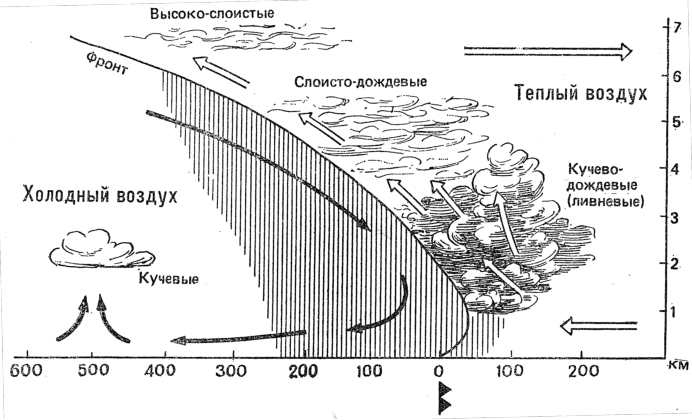
\includegraphics[width=\linewidth]{0122P}
  \caption{Холодный фронт}
  \label{fig:122}
\end{figure*}

\textbf{Холодный фронт второго рода}\index{фронт!холодный!второго~рода} движется быстро и возникает при
энергичном <<подклинивании>> холодных масс под тёплые, которые
выжимаются вверх. В результате адиабатического охлаждения в них
образуются кучево\-/дождевые облака, сопровождаемые ливнями и
грозами. Холодный фронт с ливневыми облаками наступает
<<стеной>>. Впереди, в качестве предвестников фронта, быстро движутся
перисто\-/кучевые облака; ниже, в среднем ярусе, продвигаются
<<обточенные>> ветром высококучевые чечевицеобразные.

Давление непосредственно перед фронтом сильно и неравномерно падает,
судно попадает в зону ливней, гроз, шквалов\index{ветер!шквал}\index{шквал} и сильного волнения.

\textbf{Холодный фронт первого рода}
\index{фронт!холодный!первого~рода} движется медленнее по сравнению с
холодным фронтом второго рода.

Клин холодного воздуха как бы подсекает тёплые массы, вынуждая их
подниматься вверх, что приводит к образованию облачной системы. Все
процессы выражены не так бурно, как у холодного фронта второго
рода. За линией фронта имеется пелена слоисто\-/дождевых и
высокослоистых облаков, из которых выпадают обложные осадки
(рис.~\ris{122}).

\begin{figure}[!htb]
  \centering{}
  \includegraphics[width=\linewidth]{0123P}
  \caption{Схема окклюдированного циклона}
  \label{fig:123}
\end{figure}

В результате слияния тёплого и холодного фронтов возникает сложный
фронт \--- \textit{фронт окклюзии}\index{фронт!окклюзии}. Скорость
перемещения холодного фронта больше, чем тёплого. Поэтому при слиянии
фронтов тёплый воздух вытесняется вверх, образуя верхний фронт.

В зависимости от соотношения температур характер фронта окклюзии может
быть:
\begin{description}
\item[нейтрального типа] \--- вытесненные тёплые массы и облачные
  системы фронтов располагаются по фронтальным поверхностям, а
  температуры холодных масс, догоняющей и уходящей, одинаковы. При
  этом осадки постепенно ослабевают и прекращаются;
\item[тёплого типа] \--- температура массы наступающего холодного
  фронта выше температуры лежащей впереди массы. Поэтому более тёплая
  наступающая масса начинает "скользить" вперёд и вверх по поверхности
  раздела тёплого фронта;
\item[холодного типа] \--- температура наступающего холодного фронта
  более низкая. Холодные массы начинают как бы подсекать более тёплые
  и заставляют их восходить вдоль поверхности раздела холодного
  фронта.
\end{description}

Погода окклюдированного фронта тёплого типа сходна с погодой главных
тепловых фронтов, а холодного типа \--- с погодой холодных фронтов.

\textbf{Циклоны и антициклоны.}\index{циклон}\index{антициклон} Циклон
и антициклон мы рассматривали как барические области низкого\index{барический минимум} и
высокого давления\index{барический максимум}. Эти же области несут также и одну из форм
циркуляции атмосферы \--- вихреобразные воздушные возмущения. В
циклонах северного полушария эти вихри движутся по спирали против
часовой стрелки, в южном \--- по часовой, но всегда направлены к
центру циклона. Скорость ветра при этом всегда высокая. Так, в
циклонах умеренных широт она достигает 20\otdo 30~м/с,
т.\=,е. штормовой и ураганной силы, а в тропических циклонах нередко
превышает 60\otdo 70~м/с.

Погода в циклонах, особенно на линии тёплого фронта, всегда пасмурная,
облачная и прохладная, летом \--- дождливая, а зимой \--- снежная с
оттепелями. В теплом секторе молодого циклона облачности и осадков
нет, но над морем может быть и пасмурно.

Развитие циклона проходит несколько стадий: волны, молодого циклона,
окклюдированного циклона и заполненного циклона. На рис.~\ris{123}
показана схема окклюдированного циклона северного полушария.

В отличие от циклонов в антициклонах спиральные вихревые возмущения
направлены от центра антициклона. Ветровые потоки в северном полушарии
дуют по часовой стрелке, в южном \--- против часовой стрелки.

Погода в антициклоне обусловлена оседанием воздушных масс, их
адиабатическим сжатием и как следствие повышением температуры
воздуха. Поэтому летом она спокойная, характерна штилями и слабыми
ветрами, малооблачностью и безоблачностью, с резким суточным ходом
метеоэлементов. Зимой погода ясная и морозная.

\textbf{Карты погоды} (синоптические карты)
\index{карты!погоды}\index{карты!синоптические} составляют по
наблюдениям метеоэлементов на метеорологических станциях в
установленное (стандартное) время (\rris{meteo_map}).

\begin{figure*}[!htb]
  \centering{}
  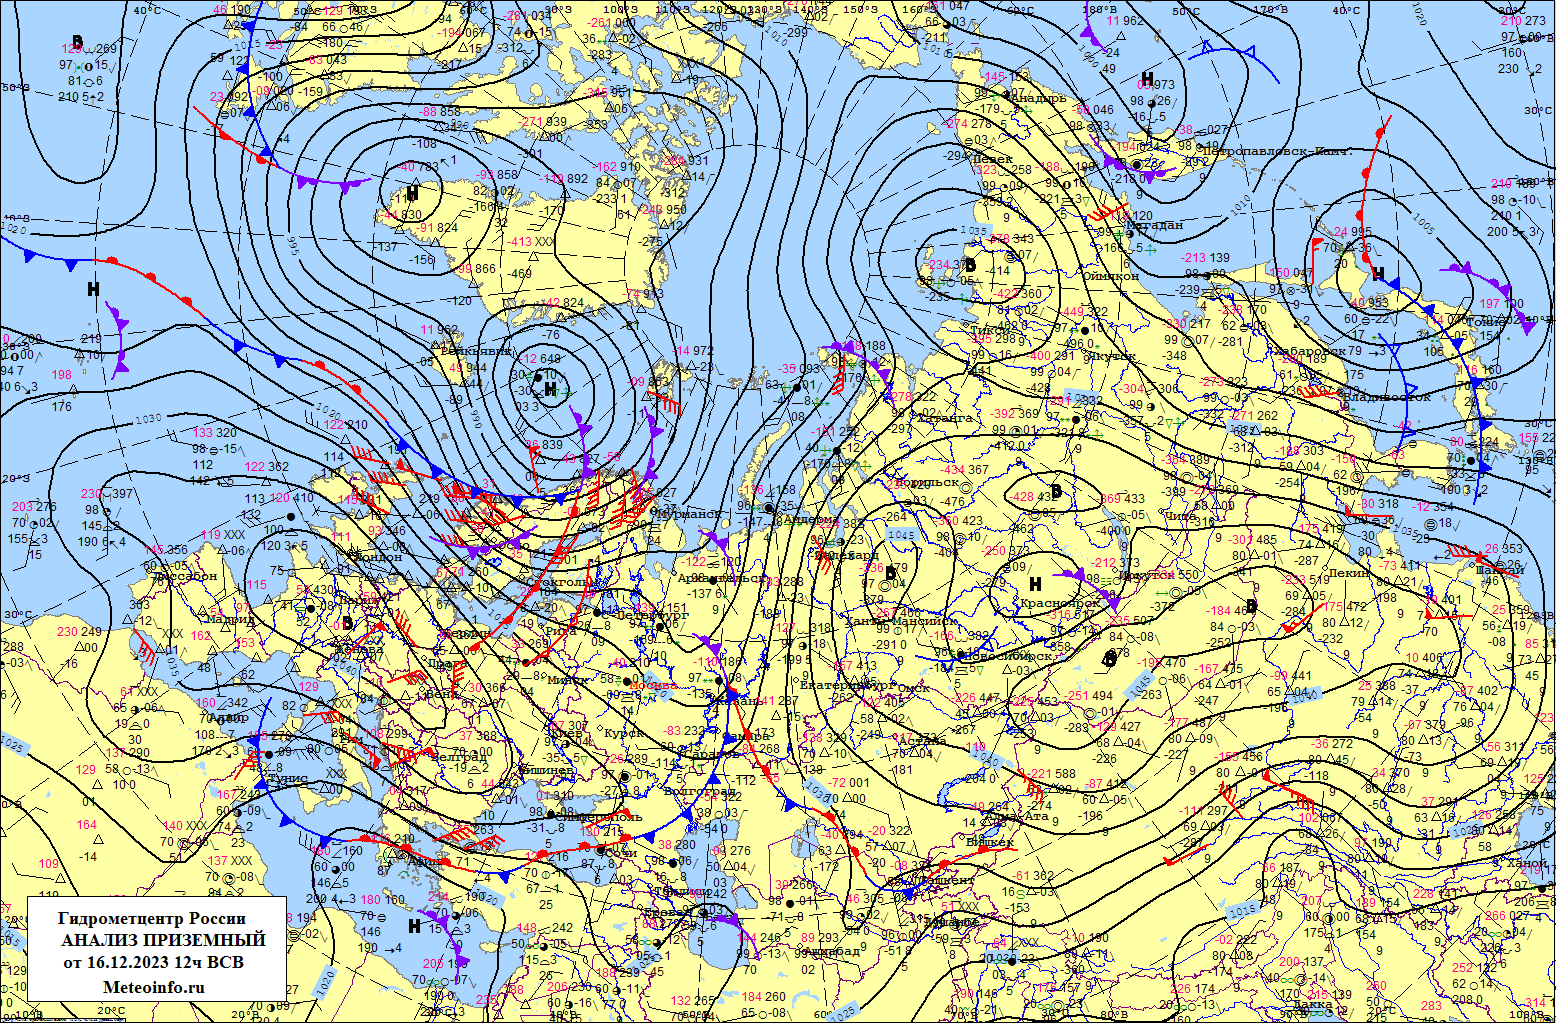
\includegraphics[width=\linewidth]{meteo_map.png}
  \caption{Синоптическая карта с фронтальным анализом}
  \label{fig:meteo_map}
\end{figure*}

Для основных (приземных) синоптических карт результаты наблюдений
снимают в 0, 6, 8 и 18 часов по Гринвичу. Раскодированную
радиоинформацию, полученную от береговых или судовых метеостанций, по
определённой схеме условными знаками наносят на специальную карту. Для
яхтенного капитана, обычно не имеющего избытка информации о погоде,
очень важно уметь определять ожидаемую погоду по местным признакам.

\section{Прогноз погоды по местным признакам, часть 1}

\begin{enumerate}
\item Ухудшение погоды (приближение циклона с тёплым фронтом:
  приближение ненастной погоды, влажной, с осадками, свежим ветром
  через 6\otdo 12~ч):
  \begin{itemize}
  \item Атмосферное давление постепенно понижается при отсутствии
    суточного хода.
  \item Нарушается суточный ход температуры воздуха, влажности\index{влажность воздуха} и ветра.
  \item Появляются быстро движущиеся от горизонта к зениту перистые
    когтевидные облака, которые постепенно сменяются
    перисто\-/слоистыми, переходящими в более плотный слой
    высокослоистых облаков.
  \item Перистые и перисто\-/слоистые облака движутся вправо от
    направления наземного ветра.
  \item Повышенная видимость, увеличение рефракции \--- появление
    предметов из-за горизонта.
  \item Усиление волнения, зыбь и волна начинают идти не по ветру.
  \item Повышенная слышимость в воздухе.
  \item Появление <<гало>> и венцов малых размеров.
  \item Сильное мерцание звёзд ночью.
  \item Утренняя заря ярко\-/красной окраски.
  \item Ночью и утром нет росы.
  \item Движение облаков нижнего и верхнего ярусов в разных направлениях.
  \item Появляются ложные солнца, миражи и т.\=,п.
  \item Вечером солнце заходит в сгущающиеся плотные облака.
  \end{itemize}
\item Ухудшение погоды (приближение холодного фронта, грозы и шторма
  за 1\otdo 2~ч до его начала).
  \begin{itemize}
  \item Резкое падение атмосферного давления.
  \item Появление перисто\-/кучевых облаков.
  \item Появление плотных разорванных перистых облаков.
  \item Появление высококучевых, башеннообразных и чечевицеобразных
    облаков.
  \item Неустойчивость ветра.
  \item Появление сильных помех в радиоприёме.
  \item Появление в море характерного шума со стороны приближения
    грозы или шквала\index{ветер!шквал}\index{шквал}.
  \item Резкое развитие кучево\-/дождевой облачности.
  \end{itemize}
\item Сохраняется плохая погода (пасмурная с осадками, сильным ветром,
  плохой видимостью) на ближайшие 6 или более часов.
  \begin{itemize}
  \item Низкое или понижающееся атмосферное давление не имеет суточного хода.
  \item Характер облачности (слоисто\-/дождевые, кучево\-/дождевые
    облака) не меняется.
  \item Температура воздуха летом пониженная, зимой повышенная, не
    имеет суточного хода.
  \item Ветер свежий, не меняет своей силы, характера и мало меняет
    направление.
  \end{itemize}
\item Улучшение погоды (после прохождения тёплого фронта или фронта
  окклюзии можно ожидать прекращения осадков и ослабления ветра в
  ближайшие 4~ч).
  \begin{itemize}
  \item Падение давления прекращается, барометрическая тенденция\index{барометрическая тенденция}
    становится положительной.
  \item Появление просветов в облаках. Высота облаков
    увеличивается. Слоисто\-/дождевые облака сменяются
    слоисто\-/кучевыми и слоистыми.
  \item Ветер поворачивает вправо и ослабевает.
  \item Волнение моря начинает успокаиваться.
  \item Местами на море появляется туман (при температуре воды ниже
    температуры воздуха).
  \end{itemize}
\item Улучшение погоды (после прохождения холодного фронта второго
  рода можно ожидать прекращения осадков, изменения направления ветра
  и прояснения через 2\otdo 4~ч).
  \begin{itemize}
  \item Резкий рост атмосферного давления.
  \item Резкий поворот ветра вправо.
  \item Резкое изменение характера облачности, увеличение просветов.
  \item Резкое увеличение видимости.
  \item Понижение температуры.
  \item Ослабление помех в радиоприёме.
  \end{itemize}
\item Сохраняется хорошая антициклоническая\index{антициклональная погода}\index{погода!антициклональная} погода (с тихим ветром или
  штилем, ясным небом или небольшой облачностью и хорошей видимостью)
  в течение ближайших 12~ч:
  \begin{itemize}
  \item Высокое атмосферное давление имеет суточный ход.
  \item Температура воздуха с утра низкая, к 15~ч повышается, а к ночи понижается.
  \item Ветер к ночи или к рассвету затихает, к 14~ч усиливается; до
    полудня поворачивает по солнцу, после полудня \--- против солнца.
  \item В прибрежной полосе наблюдаются правильно сменяющиеся утренние и вечерние бризы\index{бриз}.
  \item Появление по утрам отдельных перистых облаков, исчезающих к полудню.
  \item Ночью и утром роса на палубе и других предметах.
  \item Золотистые и розовые оттенки зари, серебристое сияние на небе.
  \item Сухая мгла у горизонта.
  \item Образование наземного тумана по ночам и утрам и исчезновение
    после восхода солнца.
  \item Солнце опускается на чистый горизонт.
  \end{itemize}
\item Характер погоды сохраняется на ближайшее время.
  \begin{itemize}
  \item Повторение в сроки наблюдений метеоэлементов прошедшего дня.
  \item Вид облачности, видимость, характер осадков, цвет неба,
    окраска зари, слышимость радиоприёма, состояние моря, тип и
    характер волнения, оптические явления в атмосфере похожи на такие
    же признаки прошедшего дня.
  \end{itemize}
\end{enumerate}

В заключение уместно вспомнить некоторые мнемонические морские
поговорки, которые облегчали морякам борьбу с морской стихией в давние
времена, когда каждый капитан <<был сам себе бюро погоды>>.

\small

\begin{quote}
Ходят чайки по песку \\*
Моряку сулят тоску. \\*
И пока не сядут в воду, \\*
Штормовую жди погоду.
\end{quote}

\begin{quote}
Барашки по небу бегут, \\*
Иль небо мётлами метут, \\*
Когда рангоут твой высок, \\*
Оставь лишь марсели да фок!
\end{quote}

\begin{quote}
Лезет стрелка вверх упорно, \\*
Не желая отдохнуть, \\*
Можешь ждать тогда бесспорно, \\*
Что от ОСТа будет дуть!\footnote{Для северного полушария}
\end{quote}

\begin{quote}
  При низком барометре\index{барометр} \--- \\*
  первый подъём, \\*
  Шквалов\index{ветер!шквал}\index{шквал} здоровых, бесспорно, \\*
  мы ждём.
\end{quote}

\begin{quote}
Если стрелка вдруг упала. \\*
Жди грозы, дождя иль шквала\index{ветер!шквал}\index{шквал}; \\*
Если ж стрелка поднимается, \\*
То погода улучшается.
\end{quote}

\begin{quote}
Скачет стрелка вверх и вниз \\*
То погоды лишь каприз \\*
Если ж медленно движенье \--- \\*
Жди надолго измененья.
\end{quote}

\begin{quote}
Если тучи громоздятся \\*
В виде башен или скал, \\*
Скоро ливнем разразятся, \\*
Налетит жестокий шквал\index{ветер!шквал}\index{шквал}.
\end{quote}

\begin{quote}
Если сгрудятся тучи и быстро летят, \\*
Скоро все снасти твои затрещат. \\*
Если на клочья начнут они рваться \--- \\*
Ставь брамселя: их не стоит бояться!
\end{quote}

\begin{quote}
Вечером небо коль полно огня, \\*
Утром же зорю туман застилает \\*
Верные признаки ясного дня, \\*
Старый моряк парусов прибавляет.
\end{quote}

\begin{quote}
  Птицы коль к берегу \\*
  держат свой путь \--- \\*
  Ветер здоровый, \\*
  поверь, будет дуть!
\end{quote}

\begin{quote}
Дождик раньше, ветер вслед \--- \\*
Жди от шквала\index{ветер!шквал}\index{шквал} всяких бед! \\*
После ветра дождь придёт \--- \\*
Значит, скоро шквал пройдёт.
\end{quote}

\begin{quote}
Если солнце село в воду \--- \\*
Жди хорошую погоду, \\*
А когда садится в тучу \--- \\*
Берегись, получишь бучу!
\end{quote}

\normalsize

Разумеется, местные признаки погоды помогают яхтенному капитану, если
он хорошо изучил природу и физическую сущность атмосферных явлений и
процессов.

\clearpage
\section{Прогноз погоды по местным признакам, часть 2}\label{sec:ppmp}

\footnotesize{}

Составлено на основе книги: А.Е. Зубков, Предсказание погоды на море
по местным признакам, 3-е издание, М., Транспорт, 1970

В книге рассматриваются процессы, происходящие в атмосфере и
окружающей природе. Главное внимание уделено описанию явлений,
связанных с изменением физического состояния атмосферы и имеющих
важное значение для предсказания погоды на море по местным
признакам. В отличие от второго издания, в третьем более полно и
подробно освещаются три основных вопроса, практически очень важных в
судовождении: предсказание погоды, ориентирование в синоптической
обстановке на море и уклонение судов от ураганов и штормов. Книга
рассчитана на широкий круг работников морского флота, рыбной
промышленности и может быть использована учащимися морских учебных
заведений.

В интернет-публикации, ориентированной на яхтсменов и
туристов-парусников, материал книги приводится в
сокращении. Иллюстрации вида облаков плохого качества заменены
фрагментами, заимствованными из учебного пособия <<Облака>>
(А.О. Андреев, М.В. Дукальская, Е.Г. Головина, СПб, изд. РГГМУ,
2007). (Авторы фото О.А. Андреева, В.И. Боярский, О.Г. Дагаев,
О.Н. Ионова, В.С. Ипполитов, Т.В. Потапова, А.Г. Саенко и Н.Н. Якимова
указаны в этом издании без привязки к конкретным снимкам.) Авторы
других фото приведены, если были указаны в источнике. Имеющиеся в
книге поясняющие сноски открываются по ссылкам в новых окнах,
несколько пояснений добавлено.

Подготовка "--- Г. Шмерлинг

По материалам сайта \url{http://parusanarod.ru/bib/books/zubkov/index.htm}

\normalsize{}

Умение ориентироваться в метеорологической обстановке имеет большое
значение для судоводителя. Местные признаки погоды играют важную роль,
так как помогают правильному пониманию метеорологических явлений и
предсказанию погоды. Прогнозы погоды, составляемые в гидрометеоцентрах,
характеризуют развитие погоды над большими районами. Поэтому в месте
нахождения судна предсказанное прогнозом явление погоды может
наблюдаться несколько раньше или позже, или совсем не наступить, а
может наступить даже не предсказанное явление. Поэтому местные
признаки погоды имеют важное практическое значение.

В ходе изменений погоды есть свои закономерности.

Во-первых, изменения никогда не начинаются с дождя или снега; гроза,
ливень, сильный ветер и другие резкие изменения погоды не приходят и
не начинаются <<внезапно>>. Они являются конечными фазами развития
взаимосвязанных атмосферных процессов.

Во-вторых, погоде свойственна инерция, т.\=,е. способность сохранять
свои особенности. Например, если длительное время стояла жаркая, сухая
погода, то, как правило, проходит много времени, пока подойдут новые
мощные воздушные массы и создадут интенсивные процессы в атмосфере,
формирующие другие условия, например, дождливую и прохладную погоду с
сильными ветрами. Периоды такой постоянной погоды той или иной
продолжительности наблюдаются довольно часто. Поэтому существуют
признаки, свидетельствующие не только о резкой перемене погоды, но и о
сохранении прежней устойчивой погоды.

Кроме того, изменения погоды нередко происходят поэтапно. Например,
после прохождения облачности может наступить кратковременное
прояснение, а затем небо снова затягивается мощными облаками.

При соответствующих атмосферных условиях погода может резко
измениться: дождь, сильный ветер, гроза и т. д. Но бывает и так, что
заметные изменения тех или иных признаков (появление облачности,
усиление ветра и др.) не вызывают резкой перемены погоды. Поэтому при
предсказании погоды необходимо учитывать ряд признаков и некоторое
время наблюдать за ходом их изменения.

Прогноз погоды по местным признакам можно составлять на сутки и
больше, но наиболее точные результаты могут быть получены на ближайшие
3--12~ч.

Местные признаки погоды делятся на общие, обусловленные масштабными
атмосферными процессами, и специальные, зависящие от особенностей
местности. Например, падение атмосферного давления почти везде
свидетельствует о приближении циклона и ухудшении погоды, а в
Новороссийске появление в ясный солнечный день облака на Мархотском
перевале является специальным признаком, что скоро подует очень
сильный северо-восточный ветер "--- бора\index{бора}.

Внимательное наблюдение даёт возможность накопить опыт предсказания
погоды для данной местности.

Опытный моряк, хорошо знающий местные признаки погоды, по едва
уловимым явлениям может предсказать приближение шторма или
урагана. Использование местных признаков погоды при наличии опыта и
знаний метеорологии может дать хорошие результаты, но имейте в виду:
любой признак может привести к ошибочному выводу, если его
использовать отдельно от других, без понимания общего хода изменений
погоды.

Полагаться можно только на совокупность нескольких совпадающих
признаков того или иного характера изменения или сохранения
погоды. Если признаки противоречивы, следует принимать во внимание те,
которые выражены сильнее. Если признаки выражены слабо и изменяются
медленно, то и погода будет изменяться медленно, и наоборот.

Атмосферные фронты, циклоны\index{циклон} и антициклоны\index{антициклон} занимают большие
пространства и перемещаются на значительные расстояния. Поэтому первые
признаки их приближения могут быть обнаружены задолго до их прихода в
место наблюдения. Приближение холодного фронта можно обнаружить за 6--8~ч
до его прохождения, а приближение тёплого фронта за 12--20~ч и
более. О предстоящей погоде можно судить по наблюдениям за облаками,
ветром, атмосферным давлением, оптическими и другими явлениями,
происходящими в атмосфере и окружающей природе. Отметить, что в любом
случае следует пользоваться прежде всего прогнозами метеослужбы, а
местные признаки должны служить дополнением и уточнением ситуации на
месте.

\subsection{Облака}

Облака образуются на разной высоте и в зависимости от характера
воздушных течений приобретают различную форму. Образование
определённых форм облаков и их изменение характеризуют многие
атмосферные процессы и явления.

При наблюдении за облаками важно замечать: количество облаков,
характер их расположения (сплошной массой, отдельными массами, волнами
и т. д.); формы облаков; высоту их нижней и верхней границ; внешний
вид и очертания; направление и скорость перемещения.

Важно также знать, как изменяются облака с течением времени:
увеличивается или уменьшается их количество, уплотняются они или
становятся тоньше, с какой стороны горизонта они впервые появляются,
цвет облаков и т.д.

\subsubsection{Облака верхнего яруса}

Нижняя граница облаков верхнего яруса располагается на высотах более
6000~м. Они бывают видны с расстояния 100--200~км, и по ним
заблаговременно (за сутки и более) можно судить о изменении
погоды. Некоторые из этих облаков на 400--500~км опережают
приближение облаков нижнего яруса, из которых выпадают осадки.

Основными формами облаков верхнего яруса являются перистые,
перисто-слоистые и перисто-кучевые. Перистые облака могут служить
признаками как плохой (циклональной\index{циклональная погода}\index{погода!циклональная}),
так и хорошей (антициклональной\index{антициклональная погода}\index{погода!антициклональная})
погоды. Это зависит от их вида, количества, расположения, направления
и скорости движения. Перистые облака появляются обычно с той стороны,
откуда идёт циклон. Известны следующие признаки предсказания погоды по
перистым облакам.

\p{1} Если перистые облака в виде нитей, когтей, нитей с крючками
(\rris{pp01}) надвигаются и уплотняются, а их количество возрастает,
то следует ожидать сильного ветра, осадков, плохой видимости,
т.\=,е. ненастной погоды. Быстрое движение этих облаков указывает на
большую скорость перемещения фронта циклона; в этом случае ненастная
погода возможна через 10--12~ч. Если же облака движутся медленно,
уплотняются и снижаются, ненастная погода с сильными ветрами возможна
через 1--3~суток. Если этих облаков мало и они рассеяны по небу,
то это означает, что в данном районе неустойчивая погода в ближайшие
6--12~ч будет с переменной облачностью, без осадков, со слабыми и
умеренными ветрами.

\begin{figure}[htb]
  \centering{}
  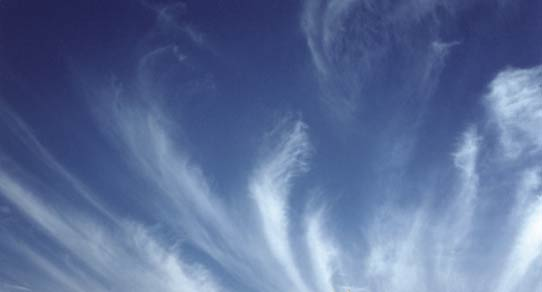
\includegraphics[width=\linewidth]{PP-01.jpeg}
  \caption{Перистые нитевидные и когтевидные облака}
  \label{fig:pp01}
  \small
  \centering{}
\end{figure}

\p{2} Если после прохождения циклона над разорванными кучевыми
облаками видны быстро движущиеся перистые облака, то это признак
приближения нового циклона; улучшение погоды будет
кратковременным. Можно ожидать изменения направления ветра от
северо-западного к юго-восточному.

\p{3} Беспорядочно рассеянные по небу перистые облака (\rris{pp02}),
почти неподвижные, похожие на тонкие растрёпанные куски ваты (их
количество со временем не увеличивается), появляющиеся после полудня и
исчезающие к вечеру "--- признак установившейся хорошей погоды. Они
наблюдаются в центральной части антициклона иди в отроге высокого
давления.

\begin{figure}[htb]
  \centering{}
  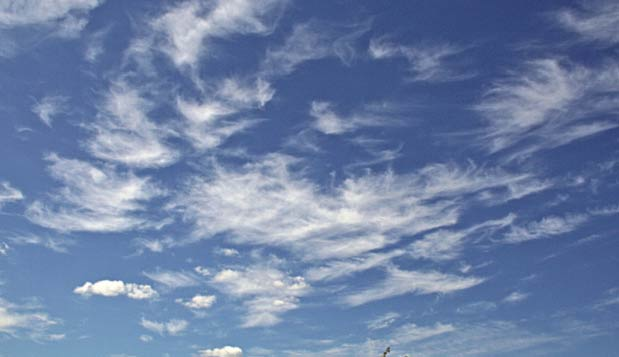
\includegraphics[width=\linewidth]{PP-02.jpeg}
  \caption{Перистые облака хорошей погоды}
  \label{fig:pp02}
  \small
  \centering{}
\end{figure}

\p{4} Тонкие, прозрачные перисто-слоистые облака, постепенно
заволакивающие весь небосвод беловатой нежной пеленой, лишь слегка
ослабляющей лучи солнца (\rris{pp03}) "--- признак приближения тёплого
фронта циклона или фронта окклюзии
%\footnote{Фронты окклюзии
%  образуются в тылу циклона, когда сливаются холодный и тёплый
%  фронты. Тёплый воздух уже не соприкасается с поверхностью
%  Земли. Фронты окклюзии бывают холодного (\rris{pp-n4-2}) и теплого
%  (\rris{pp-n4-1}) типов. Летом в средней полосе наблюдаются холодные
%  фронты окклюзии (в тыл циклона поступает холодный арктический
%  воздух), зимой — теплые (в тыл циклона поступает более теплый
%  морской воздух).}
типа тёплого фронта; следует ожидать обложных
осадков, усиления ветра через 12--23~ч, а иногда в течение ближайших
6--12~ч.

%\begin{figure}[htb]
%  \centering{}
%  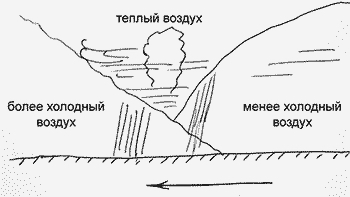
\includegraphics[scale=0.8]{PP-N4-1.jpeg}
%  \caption{Фронт окклюзии теплого типа}
%  \label{fig:pp-n4-1}
%\end{figure}

%\begin{figure}[htb]
%  \centering{}
%  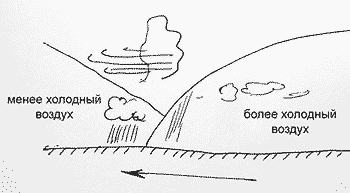
\includegraphics[scale=0.8]{PP-N4-2.jpeg}
%  \caption{Фронт окклюзии холодного типа}
%  \label{fig:pp-n4-2}
%\end{figure}

\begin{figure}[htb]
  \centering{}
  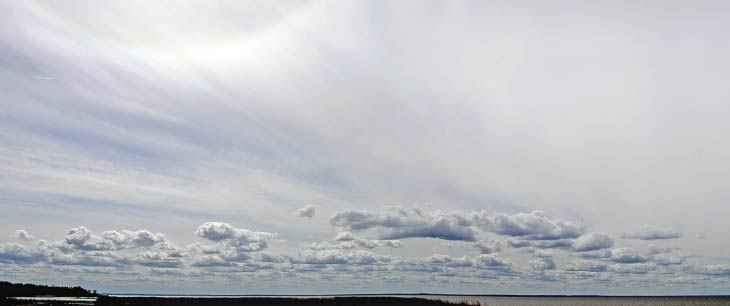
\includegraphics[width=\linewidth]{PP-03.jpeg}
  \caption{Перистo-слоистые облака}
  \label{fig:pp03}
  \small
  \centering{}
\end{figure}

\p{5} Если количество перистых или перисто-слоистых облаков не
увеличивается или они постепенно исчезают, причём бывает видно
перемещение их базы\footnote{База облаков "--- место их наибольшего
  скопления на небосводе} вдоль горизонта, это значит,. что циклон
проходит в стороне; существенных изменений в погоде в ближайшие
12--24~ч можно не ожидать.

\p{6} Если перистые облака появляются в виде «шапок» и «покрывал» над
вершинами кучевых облаков, то в ближайшие 6--12~ч нужно ожидать
переменную погоду с проходящими ливневыми осадками и сильными ветрами.

\p{7} Вытягивание перистых облаков в виде длинных узких полос, выходящих
из одной точки горизонта, означает, что в ближайшие 6--12~ч выпадут
обильные осадки и подует сильный штормовой ветер. Такая форма перистых
облаков образуется при очень сильном ветре на высотах, где они
располагаются.

\p{8} Появление большого количества плотных перистых облаков при
высокой влажности\index{влажность воздуха} и высокой температуре воздуха, когда становится
душно и «парит», означает возможность ливневого дождя и грозы в
ближайшие 6\otdo12~ч.

\p{9} Отдельные перистые облака без крючков, коготков или комков на
конце, разбросанные по небу, кажущиеся неподвижными, которые отделены
от горизонта полоской голубого неба, появляющиеся по утрам и
исчезающие к полудню "--- признак сохранения устойчивой хорошей погоды
со слабыми или умеренными ветрами и хорошей видимостью.

\p{10} Если одновременно наблюдаются перистые и кучево-дождевые
облака, то последние приобретают форму наковальни, что указывает на
возможность ливня в ближайшие часы.

\p{11} Перистые облака, быстро движущиеся с западной или южной
стороны, предвещают наступление в ближайшие 6--12~ч продолжительной
ненастной погоды с сильными ветрами и осадками (приближение
центральной части циклона).

\p{12} Если движение перистых облаков медленное, у горизонта видно
место их скопления (\textit{база}\index{облака!база}), форма их однообразна и изменяется мало,
замечается таяние облаков, то предстоящая погода будет с временным
увеличением облачности, но без осадков.

\p{13} Перисто-кучевые облака, покрывающие все небо или большую его
часть, всегда указывают на приближение холодного фронта или окклюзии
типа холодного фронта, осадков и свежего или штормового (возможно со
шквалом\index{ветер!шквал}\index{шквал}) ветра в ближайшие сутки.

\p{14} Если количество перисто-кучевых облаков постепенно
увеличивается, следует ожидать ливневых осадков, сильных ветров с
последующим похолоданием.

\p{15} Если количество перисто-кучевых облаков не увеличивается или
они постепенно исчезают, то холодный фронт или окклюзия типа холодного
фронта, циклон или ложбина низкого давления проходят в стороне.

\p{16} Если перисто-кучевые облака наблюдаются утром или днем, а к вечеру
появляются слоисто-кучевые облака, то это означает, что ночью возможна
гроза и сильный ветер.

\p{17} Если края отдельных перисто-кучевых облаков (барашков) резко
очерчены и промежутки между ними увеличиваются, то осадков не будет.

\p{18} Когда края отдельных перисто-кучевых облаков расплывчаты и
соприкасаются друг с другом, в ближайшие часы можно ожидать выпадения
осадков, усиления ветра.

\p{19} Перисто-кучевые облака в виде мелкой ряби, быстро движущиеся,
появляющиеся вместе с движущимися перистыми или перисто-слоистыми
облаками, предвещают в ближайшие 6--12~ч прохождение шквала\index{ветер!шквал}\index{шквал}, часто
сильного, иногда без низких облаков и осадков, с последующим
похолоданием.

\subsubsection{Облака среднего яруса}

Облака среднего яруса располагаются на высотах от 2000 до 6000~м. Они
опережают приближение облаков нижнего яруса на 200--300~км. От облаков
верхнего яруса эти облака внешне отличаются более крупными составными
элементами, большей плотностью, более серым цветом и наличием теней;
свет солнца и луны сквозь них проходит слабо или вообще не
проходит. Основные формы этих облаков "--- высококучевые и
высокослоистые. Высококучевые облака довольно разнообразны по
форме. Наиболее характерные из них представляют собой плотные белые,
иногда сероватые или синеватые волны (гряды), состоящие из пластов,
похожих на плиты или крупные хлопья. Эти облака предвещают наступление
холодного фронта или фронта окклюзии типа холодного фронта. Система
облаков холодного фронта обычно имеет сравнительно небольшую ширину
(примерно 100--120~км).

\p{20} Если высококучевые облака надвигаются от одной стороны
горизонта, при наличии у самого горизонта других облаков (обычно
вершин кучево-дождевых), то это свидетельствует о приближении
холодного фронта, свежего и штормового ветра, выпадении в ближайшие
2--4~ч ливневых осадков.

\p{21} Если вслед за перистыми и перисто-слоистыми облаками появляются
высококучевые с расплывчатыми краями, постепенно сливающиеся в
сплошной облачный слой, то в ближайшие 4--8~ч наступит
продолжительная ненастная погода с осадками и свежими ветрами,
связанная с приближением и прохождением тёплого фронта или фронта
окклюзии того же типа.

\p{22} Высококучевые облака в виде сравнительно небольших, быстро
изменяющихся шаров, появляющиеся одновременно с перистыми облаками и
переходящие затем в высокослоистые или сравнительно широкие
чечевицеобразные облака (\rris{pp04}), служат признаком приближения
холодного фронта, через 12--18~ч. реже "--- в ближайшие 6--12~ч
можно ожидать ливневых осадков, иногда с грозой, штормового ветра с
последующим резким похолоданием.

\begin{figure}[htb]
  \centering{}
  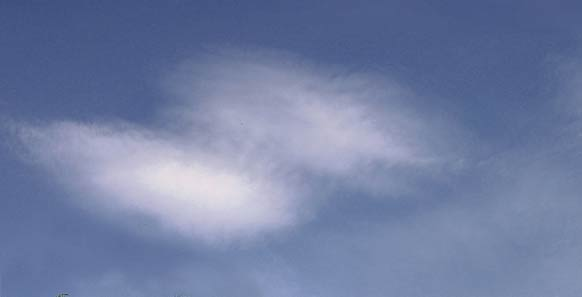
\includegraphics[width=\linewidth]{PP-04.jpeg}
  \caption{Чечевицеобразные облака}
  \label{fig:pp04}
  \small
  \centering{}
\end{figure}

\p{23} Отдельные высококучевые чечевицеобразные облака в виде узких
вытянутых форм "--- признак приближения быстродвижущегося холодного
фронта: в ближайшие 4--6~ч можно ожидать шквала\index{ветер!шквал}\index{шквал}, иногда без
облаков нижнего яруса и осадков (так называемый «белый» шквал).

\p{24} Если в просветах низких слоистых облаков видны высококучевые
облака чечевицеобразной формы с округлыми или в виде полос с ровными
резко очерченными волнообразными краями, то это признак приближения
холодного фронта или фронта того же типа; в ближайшие 6--12~ч наступит
ненастная погода со шквалами\index{ветер!шквал}\index{шквал}, ливнями, грозами (тёплое время), но она
быстро сменится похолоданием.

\p{25} Если края высококучевых облаков теряют резкость очертаний, а
отдельные облачка расплываются и сближаются друг с другом, то в
ближайшие 6--12~ч выпадут осадки и подуют свежие ветры.

\p{26} Появление высококучевых волнистых облаков в виде крупных рядов
валов, располагающихся через весь небосвод от одной стороны горизонта
до противоположной, при сильном падении давления свидетельствует, что
в ближайшие 6--10~ч следует ожидать шквалов\index{ветер!шквал}\index{шквал} и гроз, иногда при этом
могут быть смерчи\index{смерч}\index{ветер!смерч}. Такая же погода наступает после появления в высоко
кучевых облаках радужной цветной окраски параллельно краям облака.

\p{27} Появляющиеся утром над берегом, быстро движущиеся разбросанные по
всему небу высококучевые облака в виде хлопьев (\rris{pp05}) характеризуют
весьма сильную неустойчивость в средних слоях тропосферы и предвещают
в послеполуденные часы возможную грозу или ливневые осадки, сильный
ветер.

\begin{figure}[htb]
  \centering{}
  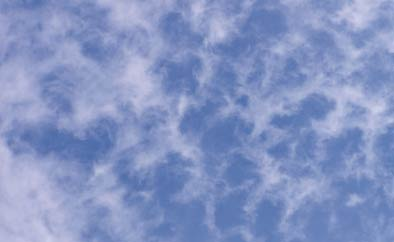
\includegraphics[width=\linewidth]{PP-05.jpeg}
  \caption{Высококучевые облака}
  \label{fig:pp05}
  \small
  \centering{}
\end{figure}

\p{28} Наблюдаемые утром в прибрежной зоне высококучевые облака с
выступающими вверх башенками "--- башенковидные облака (\rris{pp06}) "--- признак
грозы, штормового ветра во второй половине дня или вечером.

\begin{figure}[htb]
  \centering{}
  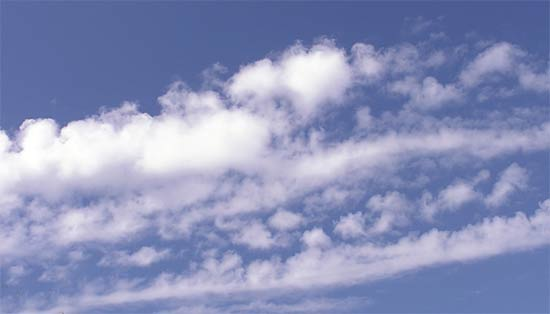
\includegraphics[width=\linewidth]{PP-06.jpeg}
  \caption{Башенкообразные облака}
  \label{fig:pp06}
  \small
  \centering{}
\end{figure}

Высокослоистые облака на море и на суше всегда связаны с системой
облаков тёплою фронта или окклюзии типа тёплого фронта Очень часто они
являются непосредственным продолжением снижающегося и уплотняющегося
покрова перисто-слоистых облаков.

\p{29} Переход перистых облаков в высокослоистые (\rris{pp07}) и
дальнейшее их уплотнение и снижение при устойчивом падении
давления "--- признак (обычно в ближайшие 6--12~ч) выпадения
осадков и наступления ветреной погоды. Ненастная погода длится 12~ч и
более. Затем облачный слой поднимается выше, становится тоньше и
распадается на пластинки высококучевых облаков с увеличивающимися
просветами между ними.

\begin{figure}[htb]
  \centering{}
  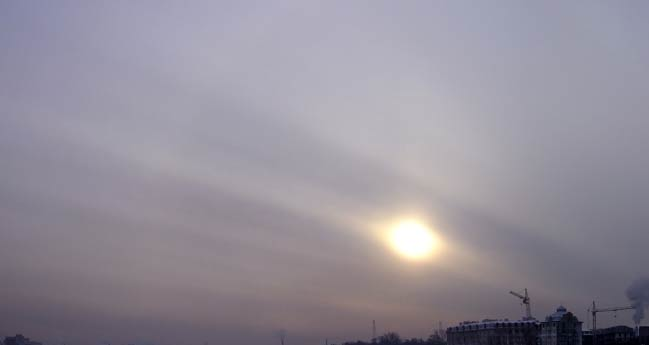
\includegraphics[width=\linewidth]{PP-07.jpeg}
  \caption{Высокослоистые облака}
  \label{fig:pp07}
  \small
  \centering{}
\end{figure}

\p{30} Если снижение высокослоистых облаков прекращается и они
приобретают форму плотных высококучевых, то предстоящая погода будет
со слабыми обложными осадками, со слабыми и умеренными ветрами.

\p{31} Сплошная пелена высокослоистых просвечивающихся облаков,
образовавшаяся из высококучевых (при этом в течение суток наблюдается
многократный переход высокослоистых облаков в высококучевые и
наоборот), признак того, что в ближайшие 12--16~ч наступит погода
с переменной облачностью, без осадков, со слабыми или умеренными
ветрами.

\subsubsection{Облака нижнего яруса}

Облака нижнего яруса имеют вид низких серых и тёмных тяжёлых гряд,
валов, а иногда сплошной пелены. Лучи Солнца сквозь них не проходят,
лишь изредка слабо просвечивают через наименее плотные края. Облака
нижнего яруса могут быть слоисто-кучевыми, слоисто дождевыми и
слоистыми. При наличии сплошных слоистых или слоисто-кучевых облаков,
когда не видно их верхних слоев, необходимо обращать внимание на
изменение цвета облаков, на уплотнение и снижение облачности и следить
за общим изменением характера погоды.

\p{32} Если появившаяся в значительном количестве (покрывающая большую
часть или все небо) слоистая облачность нижнего яруса уплотняется,
снижается, её окраска темнеет, освещённость уменьшается, давление при
этом непрерывно понижается, ветер постепенно усиливается, значит
данная облачность находится очень близко от линии тёплого
фронта. Следовательно, в ближайшие часы выпадут обложные осадки и
усилится ветер.

\p{33} При просветлении низкой слоистой облачности и устойчивом
повышении давления можно ожидать в скором времени уменьшения
облачности и общего улучшения погоды.

\p{34} Слоисто-кучевые облака (\rris{pp08}), образующиеся к вечеру из
дневных кучевых облаков, не являются признаком ухудшения погоды. Они
нередко имеют вид дождевых облаков, но быстро исчезают. Это
наблюдается при антициклонах в районах. между центром и периферией
(большей частью в западной его половине), в промежуточном барическом
образовании\index{барическое образование},
интенсивность которого ослабевает, а также в слабом,
неглубоком циклоне. При этом следует ожидать перехода к циклональной
погоде в ближайшее 12--24~ч.

\begin{figure}[htb]
  \centering{}
  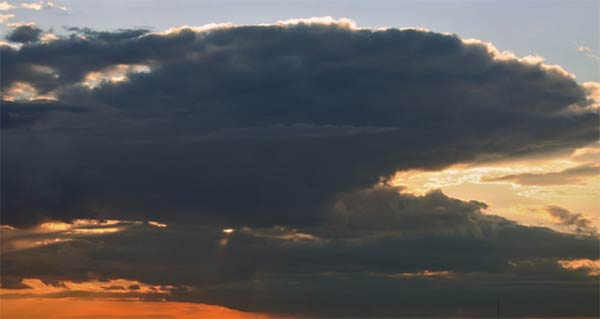
\includegraphics[width=\linewidth]{PP-08.jpeg}
  \caption{Слоисто-кучевые вечерние облака}
  \label{fig:pp08}
  \small
  \centering{}
\end{figure}

\p{35} Если летом наблюдаются слоисто-кучевые облака в форме
горизонтальных полос светло-серого цвета с неравномерными тёмными
краями, то следует ожидать холодных сильных ветров и установления в
ближайшие часы холодной и дождливой погоды.

\p{36} Если зимой вечером, после безоблачного ясного дня небо
покрывается светло-серым слоем низких слоистых облаков, то следует
ожидать продолжительных морозов.

\p{37} Темно-серые низкие слоистые облака, располагающиеся под
светло-серым облачным покровом, предвещают значительные и
продолжительные осадки.

\p{38} Переход высокослоистых плотных непросвечивающихся облаков в
слоисто-дождевые указывает на тёплый фронт или фронт окклюзии близ
линии фронта. При этом обложные осадки и свежие ветры могут продлиться
12~ч и более

\p{39} Если при наличии сплошной пелены слоисто-дождевых облаков ветер
сильный, обложные осадки могут выпадать 6~ч и более, а если ветер
ослабевает (обычно довольно резко), то следует ожидать сравнительно
скорого прекращения осадков.

\p{40} Если слоисто-дождевые облака переходят в высокослоистые или
высококучевые, осадки ослабевают, то это тыловая часть холодного
фронта или фронта окклюзии (ближайшая к центру тыловая половина
циклона или ложбины) и следует ожидать дальнейшего улучшения погоды.

\p{41} Если после прохождения слоисто-дождевых облаков и прекращения
осадков небо покрывается сплошной пеленой плотных слоисто-кучевых
облаков в виде тяжёлых валов, то это ближайшая к центру треть тыловой
половины циклона или ложбины (тыловая область холодного фронта или
фронта окклюзии). При этом следует ожидать постепенного (иногда очень
медленного) уменьшения облачности, и в течение ближайших 6--12~ч
осадки выпадать не будут.

\p{42} Если в сплошной пелене слоисто-кучевых облаков появляются
просветы, которые увеличиваются (иногда через эти просветы видны
перистые облака другого циклона или ложбины), то это приблизительно
средняя часть тыловой половины циклона или ложбины; можно ожидать, что
хорошая погода продлится 6--10~ч и более.

\p{43} Прояснение за уходящими слоисто-кучевыми облаками, границы
которых иногда бывают резко очерчены (иногда видны перистые облака
другого циклона или ложбины), предвещает хорошую погоду в течение 6~ч
и более.

\p{44} Слоисто-кучевые чечевицеобразные облака, наблюдающиеся под
высококучевыми чечевицеобразными и перисто-кучевыми облаками "---
вестники мощных ливневых облаков быстро движущегося холодного
фронта. Следует ожидать в ближайшее же время выпадения ливневых осадков
с последующим похолоданием и усилением ветра, часто до штормового и
шквалистого\index{ветер!шквал}\index{шквал}.

\p{45} Низкие слоистые облака, наблюдаемые ночью и утром, в начале дня
переходящие в кучевые "--- признак наступления в ближайшие 4--8~ч
переменной погоды с ливневыми осадками и сильными ветрами, связанными
с холодным фронтом или фронтом окклюзии.

\p{46} Если низкие слоистые облака, покрывающие все небо, не
рассеиваются к полудню, а иногда и в течение целых суток, то это
значит, что через данное место проходит слабо выраженный антициклон,
или какое-либо промежуточное барическое образование\index{барическое образование}, или старый
заполняющийся циклон. Следует ожидать моросящих дождей при слабом
ветре или штиле. Такая погода может длиться 12~ч и более.

\p{47} Сплошная пелена низких слоистых облаков (иногда с моросящими
осадками) при ветре умеренной силы, не рассеивающихся к полудню, а
часто и в течение целых суток, означает, что здесь проходит периферия
(чаще западная) антициклона или тёплого сектора нового циклона; можно
ожидать, что данный характер погоды может продлиться 6~ч и более с
последующим усилением ветра и возможным выпадением осадков.

\p{48} Разорванно-дождевые\footnote{Разорванно-дождевые облака
  представляют собой неправильные и беспорядочно разбросанные обрывки
  серых, мрачных низких облаков с изорванными под действием ветра
  краями.} облака (или облака плохой погоды), быстро движущиеся под
большим кучево-дождевым облаком, или под слоем слоисто-дождевых, или
высокослоистых, или плотных слоисто-кучевых облаков "--- верный
признак, что в ближайшее время наступит ненастная ветреная погода с
осадками При этом осадки выпадают не из разорванно-дождевых, а из
вышерасположенных облаков.

\p{49} Если зимой стоит ясная погода, а к вечеру, при штиле, небо
затягивается низкой пеленой слоистых облаков, вновь рассеивающихся
утром, то это признак тихой антициклональной погоды.

\subsubsection{Облака вертикального развития}

Основания облаков вертикального развития находятся обычно ниже 2000~м,
а вершины иногда достигают 6000--8000~м. Облака имеют вид плотных
облачных масс с плоским основанием. Вершины этих облаков всегда белые,
основание белого, сероватого или темно серого цвета.

Облака вертикального развития подразделяют на кучевые и
кучево-дождевые. Они обычно образуются над обширными пространствами
моря на сравнительно небольшом расстоянии друг от друга и имеют почти
одинаковые размеры. Основания, а часто и вершины облаков вертикального
развития над морем лежат ниже, чем над сушей

Так как на море суточная температура подстилающей поверхности, а также
температура и влажность воздуха\index{влажность воздуха} изменяют я незначительно, облака
вертикального развития в холодных воздушных массах образуются и днем и
ночью (чаще ночью) Над материками и островами, если эти облака не
связаны с атмосферным фронтом, они образуются только днем С мощными
кучевыми и кучево-дождевыми облаками связано прохождение шквалов\index{ветер!шквал}\index{шквал},
которые бывают наиболее сильными при штилевой или маловетреной погоде.

\p{50} Кучевые облака, не увеличивающиеся в высоту, располагающиеся
примерно на одинаковой высоте с резко очерченными со всех сторон
краями и плоскими основаниями (\rris{pp09}) и выделяющиеся на фоне
голубого неба, на берегу и на море "--- надёжный признак установившейся
продолжительной хорошей погоды.

\begin{figure}[htb]
  \centering{}
  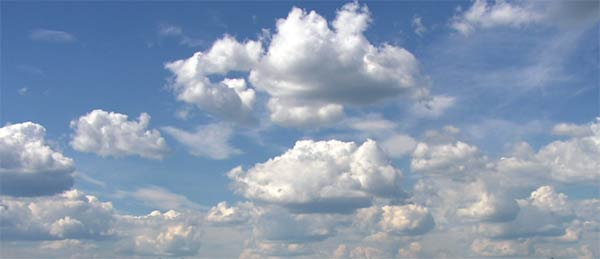
\includegraphics[width=\linewidth]{PP-09.jpeg}
  \caption{Кучевые облака хорошей погоды}
  \label{fig:pp09}
  \small
  \centering{}
\end{figure}

\p{51} Если кучевые облака, появившиеся утром над берегом и островами,
к вечеру не исчезают, а наоборот, увеличиваются, то ночью или к утру в
этих районах погода может резко ухудшиться.

\p{52} Если размеры кучевых облаков быстро увеличиваются до громадных
гор высотой в несколько километров, то в ближайшие 4--8~ч можно ожидать
превращения их в кучево-дождевые облака, выпадения ливневых осадков,
появления сильного ветра, возможно, и шквалов\index{ветер!шквал}\index{шквал}.

\p{53} Если кучевые облака приобретают форму слоисто-кучевых с
разорванными краями, при этом их вершины в северном полушарии
отклоняются вправо, а в южном—влево от направления движения, следует
ожидать при устойчивом падении давления возможного установления в
ближайшие 6--12~ч продолжительной ненастной ветреной погоды с
осадками.

\p{54} Появление у кучевых облаков внизу темно синей окраски указывает
на переход их в кучево-дождевые облака, а это означает, что в скором
времени выпадут ливневые осадки и вообще наступит ненастная погода.

\p{55} Если очень большое кучевое облако переходит в кучево-дождевое и
в верхней части от него отходят перистые облака или облако расширяется
в виде гриба или наковальни, следует ожидать в ближайшие часы грозы,
ливня и, возможно, шквала\index{ветер!шквал}\index{шквал}. Кучево-дождевые облака образуются обычно на
основе кучевых в результате сильной конвекции при интенсивном
нагревании солнцем подстилающей поверхности, либо в результате
быстрого движения холодного фронта, бурно вытесняющего вверх тёплый,
влажный и относительно лёгкий воздух. Часто наблюдаются сравнительно
редкие облака, которые при прохождении холодного фронта скапливаются
или даже образуют облачный вал. Из кучево-дождевых облаков идут ливни,
нередко сопровождаемые грозой, сильным ветром и шквалами.

\p{56} Кучево-дождевое облако у горизонта в виде гриба или наковальни
(\rris{pp10}), от вершины которой веером расходятся перистые облака,
служит признаком наступления близкой грозы, сильного шквалистого\index{ветер!шквал}\index{шквал} ветра
или града.

\begin{figure}[htb]
  \centering{}
  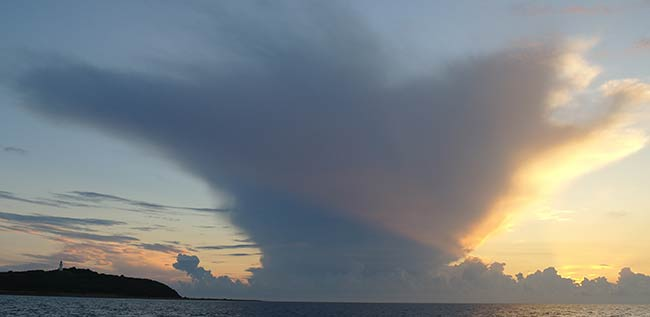
\includegraphics[width=\linewidth]{PP-10.jpeg}
  \caption{Кучево-дождевое облако с наковальней}
  \label{fig:pp10}
  \small
  \centering{}фото: Г.Шмерлинг
\end{figure}


\p{57} Если приближение громадного кучево-дождевого облака с низким
основанием и довольно высокой вершиной сопровождается духотой, что
говорит о большой абсолютной влажности воздуха\index{влажность воздуха}, то в ближайшие часы
нужно ждать грозу с ливневыми осадками.

\p{58} Если кучево-дождевое облако имеет пепельный цвет и на переднем
его крае хорошо заметны белые полосы, то надо ожидать в самое
ближайшее время обильного ливневого дождя с сильным градом и грозой
Приближение такого облака сопровождается непрерывными раскатами грома,
переходящими в рокот.

\p{59} Тёмный дугообразный облачный вал, так называемый грозовой
воротник или грозовой вал (\rris{pp11}), в передней части огромного
кучево-дождевого облака—верный признак скорого прохождения шквала\index{ветер!шквал}\index{шквал} с
ливнем, грозой, а иногда и с градом или с образованием смерча\index{смерч}\index{ветер!смерч}. При этом
после выпадения осадков обычно наступает резкое похолодание, так как
обычно такие облака и связанные с ними явления наблюдаются при
прохождении холодного фронта.

\begin{figure}[htb]
  \centering{}
  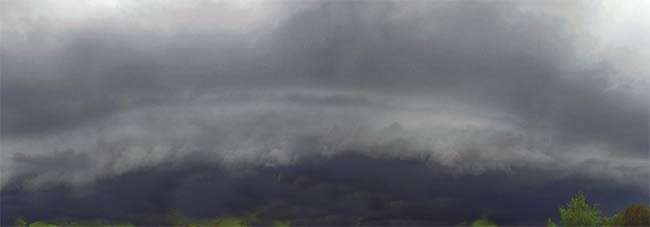
\includegraphics[width=\linewidth]{PP-11.jpeg}
  \caption{Кучево-дождевое облако с грозовым валом}
  \label{fig:pp11}
  \small
  \centering{}
\end{figure}

\p{60} В тёмном кучево-дождевом облаке грозовой вал с опускающимся
V-образным выступом-отростком (\rris{pp12}) "--- признак начала образования
смерча\index{смерч}\index{ветер!смерч} или торнадо. Возникают смерчи (\rris{pp13}) и торнадо в средних и
низких широтах из оснований мощных кучево-дождевых (грозовых) облаков.

\begin{figure}[htb]
  \centering{}
  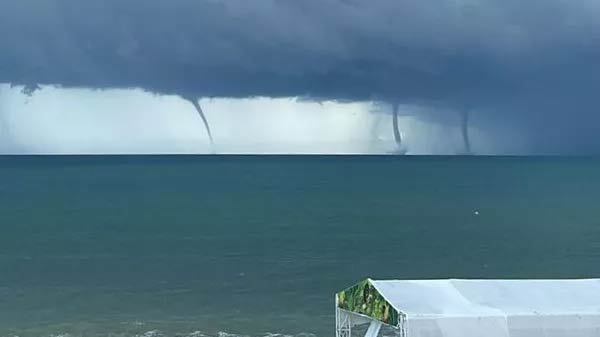
\includegraphics[width=\linewidth]{PP-12.jpeg}
  \caption{Кучево-дождевое облако со смерчами}
  \label{fig:pp12}
  \small
  \centering{}Туапсе, РИА Новости, 11.07.23
\end{figure}

\begin{figure}[htb]
  \centering{}
  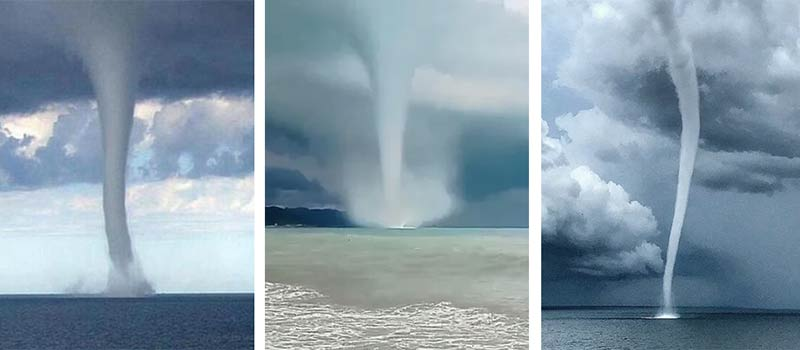
\includegraphics[width=\linewidth]{PP-13.jpeg}
  \caption{Разновидности форм смерчей на море}
  \label{fig:pp13}
  \small
  \centering{}
\end{figure}

\p{61} Приближение кучево-дождевого облака с темно-синим основанием "---
признак выпадения в ближайшее время ливневых осадков, с серо-стальным
основанием "--- ливневого дождя и града.

\p{62} Пересечение кучево-дождевого облака тёмными и светлыми
горизонтальными полосами предвещает сильную грозу.

\p{63} Чем выше поднимаются мощные кучевые облака и чем больше они
громоздятся друг на друга, тем вероятнее приближение прозы с сильным
ветром, шквалами\index{ветер!шквал}\index{шквал}, ливневыми осадками.

\p{64} Слоисто-кучевые облака, принимающие форму вымеобразных,
предвещают в скором времени наступление холодной погоды с осадками в
виде дождя или снега.

\p{65} Если на нижней поверхности кучево-дождевых или мощных кучевых
облаков постепенно появляются вымеобразные облака, то это указывает на
ослабление развития процесса и на начало разрушения этих
облаков. Можно ожидать, что облака могут пройти без ливня, грозы и
шквала\index{ветер!шквал}\index{шквал}.

\subsubsection{Облака на склоне хребта}

\p{66} Плотные облака, образовавшиеся на наветренном склоне горного
хребта, поднимаются выше или распадаются на отдельные части и
тают—признак уменьшения влажности воздуха\index{влажность воздуха}, ослабления или прекращения
ветра, дующего с моря; следует ожидать скорого прекращения осадков на
наветренном склоне горного хребта.

\p{67} Плотные облака, образовавшиеся на наветренном склоне горного
хребта, увеличивающиеся в объёме или даже спускающиеся ниже,
свидетельствуют об увеличении влажности воздуха\index{влажность воздуха} или усилении ветра с
моря.

\p{68} Слоисто-кучевые или высококучевые облака, появляющиеся из-за
горного хребта, свидетельствуют, что воздушные массы действуют на
подветренную сторону горного хребта не очень интенсивно; можно ожидать
в прибрежной зоне моря несильного фена\footnote{Фен "--- тёплый и
  сухой ветер, часто сильный и порывистый, дующий с гор по склонам
  вниз. В прибрежной зоне моря фен нередко достигает силы шторма.}.

\p{69} Слоисто-кучевые или высококучевые чечевицеобразные облака,
появляющиеся из-за горного хребта "--- признак интенсивного обрушения
воздушных масс на подветренную сторону горного хребта; следует ожидать
сильного или штормового фена.

\subsubsection{Движение облаков}

По скорости и направлению движения облаков можно судить об
интенсивности и направленности процессов в верхних слоях атмосферы,
которые затем проявится и в приземном слое.

\p{70} Движение облаков, особенно высоких, указывает на наличие
сильного ветра в верхних слоях атмосферы, что связано с быстрым
приближением фронта, циклона и предвещает ненастную ветреную погоду.

\p{71} Движение облаков от восточных или северных румбов обычно
указывает на установление антициклональной погоды "--- ясной,
маловетреной или штилевой с резким понижением температуры воздуха в
холодный период года (вторая половина осени, зима и первая половина
весны) и повышением температуры в тёплый период (вторая половина
весны, лето и первая половина осени).

\p{72} Быстрое движение облаков от западных или южных румбов в
северном полушарии наблюдается обычно перед наступлением циклональной
погоды.

\p{73} Если направление движения облаков отклоняется в северном
полушарии в левую сторону, а в южном "--- в правую относительно направления
ветра у поверхности земли, следует ожидать наступления
антициклональной погоды.

\p{74} Если направление движения перистых, перисто-кучевых или
высококучевых облаков отклоняется в северном полушарии в правую
сторону, а в южном "--- в левую относительно направления ветра у
поверхности земли, то это означает, что через данный район проходит
передняя часть циклона и надо ожидать значительного ухудшения погоды.

\p{75} Заметное движение облаков, противоположное направлению ветра у
поверхности земли, указывает на быстрое приближение холодного
фронта "--- следует ожидать в ближайшие часы ненастной погоды с грозой и
сильным ветром.

\p{76} Заметное отклонение движения перистых облаков вправо, почти под
прямым углом от движения кучевых м слоисто-кучевых облаков, означает
приближение тёплого фронта или фронта окклюзии; при устойчивом падении
давления в ближайшие 6--12~ч следует ожидать продолжительной ненастной
погоды с осадками и свежими ветрами. При этом чем быстрее два слоя
облаков движутся перпендикулярно друг другу, тем скорее нужно ожидать
ухудшения погоды.

\p{77} Если при ненастной погоде отдельные небольшие кучевые облака
быстро движутся по небу в том же направлении, в каком дует ветер у
земли, то скоро погода улучшится, осадки прекратятся, и ветер
ослабнет.

\p{78} Если в случае разрывов в нижней облачности наблюдаются более
высокие облака, движущиеся в одном направлении с низкими, то пасмурная
погода с низкой слоистой облачностью, туманом или моросящими осадками,
связанная с нахождением в данном районе устойчивой тёплой воздушной
массы, сохранится.

\p{79} Если направление движения низких облаков медленно поворачивает
против солнца, значит ветер стихнет и тёплая ненастная погода сменится
более холодной ненастной или наоборот.

\p{80} Если два слоя облаков нижнего яруса (верхний и нижний) быстро
движутся поперёк или навстречу друг другу "--- это признак скорого резкого
ухудшения погоды (осадки, сильный порывистый ветер).

\p{81} Если направление движения облаков, расположенных на разных
высотах, почти не изменяется, то это означает прохождение небольшой
ложбины со старой окклюзией типа тёплого фронта; в ближайшие 6--12~ч
можно ожидать погоду с временным увеличением облачности до
значительной, но без осадков, с умеренными ветрами.

\subsubsection{Состояние неба и изменение облачности}

\p{82} Если небо, бывшее много дней безоблачным, начинает покрываться
перистыми облаками, то скоро наступит пасмурная погода, возможно, с
осадками.

\p{83} Если на небе одновременно в разных направлениях движутся облака
различных форм, то состояние погоды неустойчиво, вероятны осадки,
сильные ветры, шквалы\index{ветер!шквал}\index{шквал} в ближайшие 4--8~ч.

\p{84} Просветление неба, постепенное прояснение и появление просветов
в сплошной пелене облаков, преимущественно справа в северном полушарии
и слева "--- в южном от наблюдателя, стоящего лицом против ветра,
уменьшение размеров капель дождя и его ослабление указывают на скорое
прекращение осадков, дальнейшее прояснение облачности, общее улучшение
погоды.

\p{85} Образование при ненастной погоде в конце дня в северном и южном
полушариях полосы безоблачного голубого неба на западе "--- признак
перемены погоды к лучшему (прекращение осадков, ветра).

\p{86} Появление днем различных форм облаков в большом количестве с
различной (от белой до тёмной) окраской "--- признак скорого ухудшения
погоды.

\p{87} Если днем сплошь покрытое низкими облаками небо быстро темнеет,
то в ближайшие часы выпадут осадки.

\p{88} Зимой часто небо долгое время бывает покрыто сплошными серыми
бесформенными облаками при установившейся циклональной погоде.

\p{89} Если над морем в течение всего дня не было каких-либо облаков и
темно-голубой небосвод кажется высоким, можно рассчитывать на довольно
устойчивую антициклональную погоду.

\p{90} Безоблачные вечера при штилевой погоде предвещают хороший день,
особенно летом.

\p{91} Безоблачное раннее утро в период неустойчивой переменной погоды
служит признаком близкого её ухудшения.

\p{92} Если зимой днем ясно, а к вечеру при штиле или слабом ветре все
небо покрывается туманным слоем низких слоистых облаков, то сохранится
антициклональная маловетреная погода.

\p{93} Меняющаяся облачность, образование просветов, хотя временами
все небо ещё покрывается низкими дождевыми облаками "--- признак
улучшения погоды.

\p{94} Постепенное увеличение и снижение облачности, появление
перистых облаков, затем перисто-слоистых (движение их настолько
быстрое, что заметно на глаз), высокослоистых и, наконец,
слоисто-дождевых "--- признак резкого ухудшения погоды, часто
связанного с приближением передней части циклона и прохождением его
правой части.

\p{95} Если нижний край основания облаков (особенно облаков нижнего
яруса) с течением времени, например, с утра и до 14--15~ч или с вечера
и до 2--3~ч ночи, заметно приподнимается, то это признак тихой, ясной,
малооблачной погоды без осадков, летом тёплой или жаркой, зимой
морозной. Если за это же время нижний край облаков не приподнимается и
даже опускается, то можно ожидать выпадения осадков и ухудшения погоды
в ближайшие 6--12~ч.

\p{96} Полное отсутствие облаков верхнего и среднего ярусов "--- признак
удалённости от места наблюдения атмосферных фронтов, а следовательно,
и ненастной ветреной погоды.

\p{97} Чем разнообразнее формы и виды облаков на разных высотах, тем
неустойчивее состояние атмосферы и тем на худшую погоду они обычно
указывают.

\p{98} Появляющиеся на горизонте облака являются признаком наступления
циклональной погоды в том случае, если они расположены в северном
полушарии слева, а в южном "--- справа относительно наблюдателя, стоящего
спиной к ветру.

\p{99} Если ночью на небе не видно мелких звёзд, а яркие становятся
крупнее, как бы «вобрав» в себя мелкие, то это свидетельствует о
высокой влажности воздуха\index{влажность воздуха}, сплошном покрытии неба перисто-слоистыми
облаками. Приближается циклон, наступит ненастная ветреная погода.

\subsection{Атмосферное давление}

Изменение давления во времени и пространстве определяет развитие
многих атмосферных процессов и явлений. Знание величины атмосферного
давления и её изменения имеет первостепенное значение для прогноза
погоды. Падение давления обычно означает приближение или развитие
циклона и ухудшение погоды, а повышение "--- приближение или развитие
антициклона и улучшение погоды. Нормальная (средняя) величина
атмосферного давления, приведённая к уровню моря, составляет 1013~гПа
(мбар) или 760~мм~рт.ст.

\subsubsection{Величина атмосферного давления}

\p{100} Если приведённое к уровню моря давление менее 1015~мбар летом
м 1020~мбар зимой, причём эта величина не изменяется или медленно
понижается, то это означает, что над данным районом находится область
циклонального характера. Плохая погода сохранится в течение 6--12~ч.

\p{101} Если приведённое к уровню моря давление более 1015~мбар летом
и 1020~мбар зимой, причём в течение суток мало изменяется, то это
значит, что над районом находится область антициклонального
характера. Хорошая погода сохранится в течение суток.

\p{102} При давлении от 1010~до 1020~мбар в данном районе может быть и
циклональная область, и антициклональная.

\subsubsection{Падение давления}

\p{103} Резкое отклонение стрелки барометра\index{барометр} влево при постукивании по
стеклу прибора означает ухудшение погоды.

\p{104} Если давление в течение 6--12~ч и больше непрерывно падает, можно
ожидать прохождения циклона, т.\=,е. ветреной погоды с осадками.

\p{105} Быстрое падение давления (2--3~мбар и более за 3~ч)
указывает на приближение центральной области циклона или очень
глубокого циклона "--- следует ожидать шторма. Чем быстрее падает
давление, тем скорее ухудшается погода.

\p{106} Давление падает перед прохождением через место наблюдения
тёплого фронта и тем быстрее, чем скорее приближается фронт. Если
давление продолжает медленно падать после прохождения тёплого фронта,
то это значит, что циклон углубляется; если давление остаётся на одном
и том же низком уровне (как правило, ниже 1015~мбар летом и 1020~мбар
зимой), циклон не изменяется; если же давление повышается, то циклон
заполняется. В последнем случае происходит улучшение погоды.

\p{107} Если давление с утра начинает медленно уменьшаться, а
температура и абсолютная влажность\index{влажность воздуха} одновременно возрастают быстрее
обычного, то можно ожидать осадков, а летом "--- ливня и грозы в
ближайшие 8--12~ч.

\p{108} Перед приближением холодного фронта давление сначала меняется
мало, а затем внезапно начинает быстро падать (за 1--2~ч). В зоне
фронта следует ожидать сильного ветра, шквала\index{ветер!шквал}\index{шквал}, ливневых осадков,
грозы. После прохождения холодного фронта давление значительно
повышается, а температура резко понижается.

\subsubsection{Повышение давленая}

\p{109} Если стрелка барометра-анероида\index{барометр-анероид}, расположенная в правой части
циферблата, при постукивании по стеклу прибора отклоняется вправо или
остаётся на месте, следует ожидать сохранения антициклональной погоды.

\p{110} Медленное, непрерывное и длительное (до нескольких суток)
повышение давления "--- признак установления продолжительной
антициклональной погоды: летом "--- жаркой, зимой "--- морозной.

\p{111} Если давление в течение нескольких часов поднималось и затем
остановилось, то через место наблюдения проходит отрог повышенного
давления "--- улучшение погоды будет кратковременным.

\subsubsection{Запись барографа}\index{барограф}

\p{112} Если барограмма\index{барограмма} имеет вид слабо волнистой, горизонтальной
кривой, то установившаяся погода сохранится в течение 12~ч и
более. Подобная запись характерна при движении судна <<по изобаре>>,
прохождении центральной области обширного антициклона или отрога
высокого давления.

\p{113} Если при падении давления кривая обращена выпуклостью вверх
(давление падает ускоренно), можно ожидать сильного ветра,
значительного ухудшения погоды.

\p{114} Когда кривая при падении давления обращена выпуклостью вниз
(давление падает замедленно), падение давления может прекратиться. В
этом случае следует ожидать ослабления ветра и улучшения погоды.

\p{115} Если при повышении давления кривая обращена выпуклостью вниз
(давление повышается ускоренно), ветер может усилиться. Такая запись
часто наблюдается при прохождении левой половины циклона, т.\=,е. его
внефронтальной, чаще всего северной части.

\p{116} Если при повышении давления кривая обращена выпуклостью вверх
(давление повышается замедленно), можно ожидать продолжительную
маловетреную, штилевую, ясную погоду в результате прохождения
антициклона или отрога высокого давления.

\p{117} Если запись на барограмме\index{барограмма} имеет волнообразную форму, в которой
обнаруживаются две ложбины с промежутком около 2 суток, это означает,
что через данный район проходит серия циклонов, и весьма вероятно, что
через такой же промежуток времени давление снова упадёт в связи с
очередным прохождением циклона и временным ухудшением погоды.

\p{118} Запись равномерного падения давления происходит при
приближении тёплого фронта или фронта окклюзии того же типа.

\p{119} Равномерное падение давления и затем ровный ход или увеличение
давления наблюдается на ленте барографа\index{барограф} при прохождении тёплого фронта
или фронта окклюзии того же типа.

\p{120} За 1--3~ч прохождения холодного фронта барограф\index{барограф} указывает на
падение давления. После прохождения холодного фронта кривая резко
изгибается, и барограф вычерчивает линию повышения давления.

\subsubsection{Суточный ход атмосферного давления}

В суточном ходе давления наблюдается два максимума "--- около 10~и 22~ч и
два минимума "--- около 4~и 16~ч. Эти изменения давления особенно чётко
выражены в тропических широтах. Близ экватора амплитуда суточных
колебаний давления составляет 3--4~мбар. С увеличением широты амплитуда
суточных колебаний уменьшается и уже на широте 60\gr составляет около
$0,3$~мбар. В средних и полярных широтах на фоне частого прохождения в
этих широтах циклонов и атмосферных фронтов суточные колебания
атмосферного давления незаметны.

\p{121} Если на барограмме\index{барограмма} заметен более или менее правильный суточный
ход атмосферного давления, следует ожидать продолжительной хорошей
погоды.

\p{122} В тропических широтах малейшее нарушение правильности
суточного хода атмосферного давления является одним из самых надёжных
признаков приближения тропического циклона. Это нарушение можно
наблюдать за 24--48~ч. Быстрое падение давления за 12--18~ч
предупреждает о наступлении передней части тропического циклона с
областью ураганного ветра.

\subsection{Ветер}

Смена погоды часто связана с изменением направления, скорости и
характера ветра.  Правила для ветра, устойчивого по направлению и
скорости

\p{123} Сильные ветры западных румбов в обоих полушариях обычно
наблюдаются во время устойчивой ненастной погоды.

\p{124} При северных и северо-восточных ветрах в северном полушарии
чаще всего преобладает ясная и холодная погода.

\p{125} При южном и юго-западном ветрах осенью, зимой и весной в северном
полушарии на море чаще всего устанавливается погода с низкой слоистой
облачностью и туманами.

\subsubsection{Правила для меняющегося ветра}

Правила для ветра, изменяющегося по скорости, направлению и характеру,
основаны на том, что при провождении через место наблюдения циклона
или фронта происходит поворот и изменение скорости и характера ветра.

\p{126} Если при ясной погоде ветер несколько дней подряд сохраняет
приблизительно одно и то же направление, но затем резко изменяется, то
можно ожидать погоды с осадками и сильными ветрами,
т.\=,е. циклональной погоды.

\p{127} Если ветер усиливается, становится порывистым и поворачивает в
северном полушарии по движению часовой стрелки, а в южном полушарии
"--- против движения часовой стрелки, можно ожидать ухудшения погоды.

\p{128} Усиление и поворот ветра против движения часовой стрелки
означают, что через место наблюдения проходит в северном полушарии
левая сторона циклона, а в южном "--- правая.

\p{129} Если направление ветра у поверхности земли совпадает с
направлением быстро движущихся по небу отдельных небольших кучевых
облаков, это означает, что через место наблюдения проходит тыловая
часть циклона.

\p{130} Если ветер усиливается, почти не меняя направления, а давление
при этом падает, то центр циклона пройдёт над местам наблюдения. При
прохождении центра циклона ветер ослабевает, давление, оставаясь
низким, не изменяется; после прохождения центра циклона ветер резко
усиливается и изменяет направление на противоположное, а давление
начинает быстро возрастать.

\p{131} Появление порывистого ветра, периодически стихающего до штиля,
указывает, что в дальнейшем ветер усилится.

\p{132} Внезапное ослабление штормового ветра до слабого предвещает
резкую перемену направления ветра.

\p{133} Ветер, постепенно усиливающийся и поворачивающий в северном
полушарии вправо, а в южном "--- влево от наблюдателя, указывает на
приближение тёплого фронта или фронта окклюзии тёплого типа. После
выпадения дождя или снега, т.\=,е. после прохождения фронта, ветер
резко поворачивает вправо и обычно ослабевает.

\p{134} Ветер, остававшийся почти без изменения во время ливневого
дождя или снега, резко поворачивающий в северном полушарии вправо, а
в южном "--- влево и усиливающийся до штормового или ветра ураганной
силы, связан с прохождением холодного фронта или фронта окклюзии
холодного типа.

\p{135} Изменение вращения ветра в северном полушарии по движению
часовой стрелки, а в южном "--- на обратное служит признаком возобновления
плохой погоды.

\p{136} Если после продолжительных осадков ветер значительно
усиливается, то можно ожидать скорого улучшения погоды.

\p{137} Небольшой постепенный поворот ветра в северном полушарии по
движению часовой стрелки, а в южном "--- наоборот, до полудня и в обратную
сторону после полудня "--- признак устойчивой ясной и маловетреной погоды.

\p{138} Если вслед за дождём ветер усиливается, то следует ожидать шквала\index{ветер!шквал}\index{шквал}.

\p{139} Направление ветра в течение суток периодически изменяется то
по часовой стрелке, то против, оставаясь в пределах той же самой
четверти или половины горизонта; скорость ветра периодически то
уменьшается, то увеличивается, нередко ветер имеет характер
шквалистого\index{ветер!шквал}\index{шквал}; давление то понижается, то повышается
(барограмма\index{барограмма}
волнообразная, с малой амплитудой колебаний) в обоих полушариях "---
признак прохождения чередующихся мелких ложбин и отрогов.

\subsubsection{Суточный ход скорости ветра}

Ветер имеет суточный ход. С восходом солнца скорость ветра
увеличивается и около 13--14~ч достигает наибольшего значения, после
чего убывает. Вечером и ночью наблюдается слабый ветер или штиль.

Суточные колебания скорости ветра особенно заметны летом над
сушей. Над морской поверхностью, температура которой в течение суток
изменяется незначительно, колебания скорости ветра небольшие, но по
мере приближения к берегам они увеличиваются. Ясно выраженный суточный
ход ветра наблюдается при установившейся антициклональной погоде,
особенно летом, когда суточные колебания температуры хорошо
выражены. С суточным ходом скорости ветра связано несколько надёжных
признаков предсказания погоды.

\p{140} Правильный суточный ход скорости ветра "--- признак сохранения ясной и маловетреной погоды.

\p{141} Хорошая погода летом более устойчива, если она сопровождается
в полуденные часы слабыми или умеренными ветрами.

\p{142} Нарушение правильного суточного хода скорости ветра предвещает
указывает на возможное ухудшение погоды.

\p{143} Постепенное восстановление нарушенного или исчезнувшего
суточного хода скорости ветра предвещает наступление хорошей погоды.

\p{144} Если ветер к вечеру не стихает, а усиливается, то возможно
ухудшение погоды, следует ожидать сильного ветра ночью и на следующий
день.

\p{145} Если ветер усиливается при заходе солнца и меняет направление
по движению часовой стрелки в северном полушарии и против часовой
стрелки "--- в южном, следует ожидать ухудшения погоды, сильного и
штормового ветра.

\subsubsection{Бризы}

Бриз\index{бриз} "--- это ветер, днем дующий с моря на сушу. а ночью "--- с суши на
море. Он возникает из-за различия в нагревании и охлаждении воздуха
над водной поверхностью и сушей.

\p{146} Наличие ясно выраженных бризов\index{бриз} там, где они обычно бывают "---
признак сохранения установившейся хорошей ясной погоды на берегу и в
прибрежной зоне.

\p{147} Нарушение правильной циркуляции бриза\index{бриз} служит признаком
ухудшения погоды, приближения циклона и, наоборот, установление
правильной циркуляции бриза предвещает хорошую погоду.

\subsubsection{Ветры горных побережий}

\p{148} Правильный суточный ход ветра, в горных районах в тёплый
период года: днем ветер дует от долин к вершинам гор и перевалам,
ночью "--- в обратном направлении; можно ожидать, что у данного побережья
моря хорошая погода антициклонального характера продлится 12--24~ч и
более.

\p{149} Нарушение правильной суточной смены горно-долинных ветров
предвещает приближение циклонов, т.\=,е. ухудшение погоды.

\p{150} Ветер, дующий с ледника вниз к долинам "--- признак антициклональной
погоды. Исчезновение ледникового ветра "--- признак наступления
циклональной погоды с осадками.

\subsection{Температура воздуха}

При установившейся ясной погоде наблюдается чётко выраженный суточный
ход температуры. На море летом и зимой: минимум перед восходом солнца,
максимум около 13~ч. Над сушей: минимум зимой и летом "--- перед восходом
солнца, максимум зимой "--- в 13--14~ч, летом "--- в 14--15~ч. В области
циклона из-за облачности суточный ход температуры нарушается.

\p{151} Правильный суточный ход температуры воздуха "--- признак, что
антициклональная погода сохранится на ближайшие сутки.

\p{152} Нарушение правильного суточного хода температуры воздуха "---
признак ухудшения погоды (переход к циклональной погоде).

\p{153} Равномерный суточный ход температуры воздуха наблюдается или в
центральной области, или на периферии ослабевающего антициклона, чаще
всего в западной его половине "--- можно ожидать перехода к погоде
циклонального характера в течение ближайших 12--24~ч.

\p{154} Если во время ненастной погоды температура воздуха резко
понижается, то надо ждать скорого улучшения погоды (холодный фронт
прошёл).

\p{155} Повышение температуры воздуха вечером и ночью "--- признак
приближения передней половины циклона: можно ожидать ухудшения погоды
в ближайшие 6--12~ч.

\p{156} Повышение температуры зимой и небольшое понижение летом часто
наблюдается перед прохождением тёплого фронта.

\p{157} Если на берегу вечером температура непосредственно у
поверхности земли заметно ниже, чем на высоте нескольких метров,
хорошая погода сохранится.

\subsection{Влажность воздуха}\index{влажность воздуха}

От количества водяного пара и степени его насыщения во многом зависит
состояние погоды: образование и характер облаков, осадков, гроз и
туманов. Абсолютная влажность "--- количество водяного пара в г$/$м$^3$
воздуха; она может измеряться и в единицах давления, показывая, какая
часть атмосферного давления приходится на водяной пар (парциальное
давление). Относительная влажность "--- отношение фактического содержания
водяного пара в воздухе к максимально возможному при той же
температуре. При относительной влажности 100\% воздух полностью
насыщен водяным паром и самое малое понижение температуры приведёт к
началу конденсации "--- появлению капелек воды или кристалликов
льда. Температуру, которая при некотором содержании водяных паров
будет отвечать 100\% относительной влажности, называют точкой
росы. Точка росы не может быть выше температуры воздуха. Чем больше
разница между температурой воздуха и точкой росы, тем суше воздух, и
наоборот.

\subsubsection{Изменение влажности воздуха}\index{влажность воздуха}

\p{158} Уменьшение абсолютной влажности\index{влажность воздуха} по сравнению с предыдущими
сутками за одни и те же сроки наблюдения указывает на улучшение
погоды.

\p{159} Очень малая относительная влажность\index{влажность воздуха} утром и возрастание её к
вечеру предвещает на ближайшие 12--24~ч ясную погоду.

\p{160} Если абсолютная влажность\index{влажность воздуха} увеличилась более чем на 3~мбар за
последние 6~ч, то на следующие сутки можно с некоторой вероятностью
ожидать обильных осадков.

\p{161} Быстрое и заметное возрастание абсолютной влажности\index{влажность воздуха} вместе с
повышением температуры и понижением давления воздуха предвещают
выпадение осадков, а в летнее время грозу.

\p{162} Если величина абсолютной влажности\index{влажность воздуха} летом превышает 18~мбар или
если точка росы превысит 16\grC, следует ожидать грозы.

\p{163} Большое увеличение абсолютной влажности\index{влажность воздуха} и температуры при
устойчивом падении давления означает прохождение циклона с грозой.

\subsubsection{Суточный ход влажности воздуха}\index{влажность воздуха}

При устойчивой ясной погоде влажность\index{влажность воздуха} воздуха обнаруживает заметный
суточный мод, параллельный с ходом температуры и испарения. В суточном
ходе абсолютной влажности над океанами и морями во все сезоны года, а
над сушей только в холодное время года наблюдаются один максимум и
один минимум.

Минимум влажности\index{влажность воздуха} наблюдается утром, максимум "--- около 13--14~ч. С
повышением температуры усиливается испарение и вместе с этим растёт
абсолютная влажность, но, так как увеличение влажности отстаёт от
повышения температуры, относительная влажность уменьшается "--- воздух
становится суше.

Поэтому суточный ход относительной влажности\index{влажность воздуха} обратен ходу температуры
перед восходом солнца относительная влажность имеет максимум, а в
13--14~ч "--- минимум.

\p{164} Если суточный ход абсолютной влажности\index{влажность воздуха} находится в
соответствии с ходом температуры, можно ожидать сохранения в ближайшие
12--24~ч антициклональной погоды.

\p{165} Резко выраженный суточный ход относительной влажности\index{влажность воздуха} или
усиление этого хода служит признаков улучшения погоды.

\p{166} Уменьшение суточных колебаний (суточного хода) относительной
влажности\index{влажность воздуха} или очень слабый ход при большой её величине происходит при
установившейся длительной ненастной погоде.

\subsubsection{Точка росы}

Точка росы определяется с помощью психрометрических таблиц по
предварительно вычисленному значению абсолютной влажности\index{влажность воздуха} или по
температуре воздуха и величине относительной влажности. По значению
точки росы можно предсказывать заморозки.

\p{167} Если вечером (в 20--22~ч) точка росы имеет значение ниже +2\grC, то
при штиле и отсутствии низкой облачности надо ожидать заморозок ночью
или к утру.

\p{168} При наличии облачности и ветра (даже слабого) и при увеличении
давления можно ожидать заморозка лишь в том случае, если точка росы
вечером была ниже нуля.

\p{169} При наличии облачности вечером и ночью и заметном ветре
заморозки маловероятны.

\subsection{Атмосферные осадки}

Характер и тип осадков тесно связаны с формой и структурой облаков. По
характеру выпадения атмосферные осадки подразделяются на ливневые,
обложные и моросящие. Ливневые осадки "--- очень интенсивны, но
кратковременны. Очень характерна для них внезапность начала и конца
выпадения. Выпадают из кучево-дождевых облаков над небольшой площадью
в виде крупных капель, либо мокрого снега, града, снежной или ледяной
крупы.

Обложные осадки "--- умеренные, они продолжаются от нескольких часов до
нескольких суток. Выпадают обычно из слоисто-дождевых облаков, иногда
из высокослоистых, слоисто-кучевых, слоистых и других облаков перед
прохождением тёплого фронта или фронта окклюзии тёплого типа; они
захватывают вдоль фронта большие пространства шириной до 400~км и
более.

Моросящие осадки "--- это или осадки в виде очень мелких капелек, почти
незаметных для глаза (морось), или очень мелкие снежинки. Выпадают
обычно из сплошных плотных слоистых облаков или из тумана.

\subsubsection{Дождь и снег}

\p{170} Если во время облачной с осадками погоды дождь или снег выпадает
временами и бывает довольно сильным "--- это признак улучшения погоды.

\p{171} Ослабление дождя или снега к вечеру предвещает улучшение погоды.

\p{172} Сильный дождь пли снег ночью или рано утром при слабом ветре
или штиле чаще всего предвещает солнечный день (прояснение наступает
обычно около полудня).

\p{173} Интенсивный дождь или снег утром при сильном или штормовом
ветре "--- признак плохой погоды на весь день.

\p{174} Если дождь или снег прекращается после полудня или вечером без
прояснения неба, то на следующий день надо ожидать выпадения нового
дождя или снега.

\p{175} Тёплый дождь чаще всего выпадает при уменьшении атмосферного
давления, а холодный "--- при повышении.

\p{176} Наиболее обильные снегопады и сильные метели бывают обычно при
температурах, близких к 0\grC. Чем сильнее морозы, тем менее вероятны
снегопады и метели.

\p{177} Если дождь перед ветром, надо ждать дальнейшего усиления ветра.

\p{178} Ливень при солнечном сиянии означает, что завтра опять будет дождь.

\subsubsection{Град}

Град выпадает из кучево-дождевых облаков только при положительных
температурах, чаще всего непродолжительное время и на ограниченной
площади, обычно в виде узкой полосы или двух параллельных полос.

\p{179} Выпадение града почти всегда связано с прохождением холодного
фронта или фронта окклюзии холодного типа и сопровождается грозами,
ливнями и шквалами\index{ветер!шквал}\index{шквал}, которые преимущественно проходят с западной
стороны горизонта.

\subsubsection{Роса и иней}

В ясную ночь при слабом ветре или штиле вследствие потери тепла путём
излучения земная поверхность и прилегающий к ней слой воздуха
охлаждаются. Когда температура подстилающей поверхности и температура
приземного слоя воздуха упадут ниже точки росы, произойдёт конденсация
водяного пара в виде росы (при температуре выше 0\grC) или инея. Появлению
росы и инея благоприятствуют безоблачная тихая погода, долгая ночь,
большая влажность\index{влажность воздуха} воздуха.

\p{180} Обильная роса или иней, образовавшиеся после захода солнца и
исчезающие только после восхода солнца "--- признак антициклональной
погоды. При этом, если после восхода солнца наблюдается штиль или
слабый ветер, то можно ожидать, что антициклональная погода продлится
12~ч и более, если же наблюдается умеренный ветер, то такая погода
установится на 6~ч и более

\p{181} Роса или иней, образовавшиеся после захода и исчезающие до
восхода солнца "--- признак перехода к погоде циклонального характера,
часто уже в течение ближайших 12~ч.

\p{182} Сильная вечерняя роса или иней "--- признак хорошей погоды, но
если роса образуется во время тумана, это свидетельствует о перемене
погоды к циклональной.

\p{183} Тихая ясная ночь без росы или инея "--- признак перехода в ближайшие
6--12~ч к циклональной погоде с осадками.

\subsubsection{Влага на предметах}

\p{184} Осаждение жидкой или твёрдой влаги на вертикальных предметах,
наблюдаемое чаще всего в холодный период года "--- признак
распространения на данный район тёплой устойчивой воздушной массы.
Можно ожидать продолжительной пасмурной погоды с низкой слоистой
облачностью, туманом, моросящими осадками и слабыми ветрами.

\p{185} Образование налёта влаги в тёплое время года, что случается
нечасто "--- признак обильного ливневого дождя, иногда грозы.

\subsubsection{Туманы}

Туман "--- взвесь мельчайших капелек воды в приземном слое воздуха,
из-за которой видимость становится менее 0,6~кбт
($\approx{}$100~м). Разрежённый туман, при котором горизонтальная
видимость может быть до 6~миль, называется дымкой. По условиям
образования туманы разделяют на радиационные, образующиеся вследствие
ночного охлаждения земной поверхности, адвективные, возникающие при
попадании тёплого воздуха на холодную подстилающую поверхность и
туманы испарения, образующиеся в холодное время года над тёплой водной
поверхностью.

Радиационные туманы возникают в прибрежной полосе моря и на берегу в
низких и сырых местах, расстилаясь белой пеленой; после восхода солнца
такие туманы рассеиваются. Туманы адвекции и испарения отличаются от
радиационных большой длительностью и огромными размерами
распространения. Над океанами и морями они наблюдаются как в
прибрежных, так и в открытых районах. Для предсказания погоды наиболее
важны радиационные туманы.

\p{186} Туман у земли (невысокий, до 2~м), образующийся после захода
солнца и рассеивающийся только после его восхода "--- признак, что
антициклональная погода со штилями и слабыми ветрами продлится 12~ч и
более.

\p{187} Туман, образующийся после захода солнца и рассеивающийся ещё
до его восхода "--- признак перехода к циклональной погоде в ближайшие
6--12~ч.

\p{188} Сплошной туман (при котором не видно неба), образующийся после
захода солнца при штиле или слабом ветре и рассеивающийся утром или до
полудня "--- признак того, что антициклональная погода продержится 12~ч и
более.

\p{189} Сплошной туман, образующийся в любое время суток при умеренном
ветре на море, часто появляющийся в виде надвигающейся по ветру стены
"--- признак, что такая погода продлится 6~ч и более.

\p{190} Нередко за ночь долины заполняются мощным слоем плотного
тумана, который утром приподнимается, превращается в низкие слоистые
облака и постепенно рассеивается. Иногда утром из облаков выпадают
моросящие осадки. Такой туман "--- признак сохранения тихой
антициклональной погоды на сутки и более.

\subsection{Световые явления в атмосфере}

Различные оптические (световые) явления в атмосфере обусловливаются
тем, что лучи солнца и других небесных светил, проходя через
атмосферу, испытывают рассеяние, преломление и дифракцию. В связи с
этим в атмосфере возникает ряд удивительных по красоте оптических
явлений. Отражая физические процессы в атмосфере, все они связаны с
изменением и состоянием погоды и могут сложить хорошими местными
признаками для её предсказания.

\subsubsection{Цвет неба и видимость}

Коротковолновая часть спектра (фиолетовые, голубые и синие лучи)
рассеивается в атмосфере (на микроскопических пылинках и флуктуациях
плотности воздуха) сильнее длинноволновой части (красные и оранжевые
лучи). Именно поэтому небо окрашено в голубой цвет: у горизонта оно
имеет светло-голубой тон, а в зените почти синий. Красные лучи
рассеиваются слабо, что объясняет красный цвет солнечного диска на
закате или сразу после восхода.

Когда свет рассеивают частицы, размер которых близок к длине волн или
больше их (пылинки, капельки воды и кристаллики снега), то лучи всех
цветов рассеиваются одинаково. Поэтому в запылённой атмосфере цвет
неба становится белесым. При наличии в воздухе большого количества
капелек воды или кристалликов льда небо серое и может даже получить
красноватый оттенок. Это наблюдается при прохождении фронтов или
циклонов, когда влага выносится мощными потоками воздуха высоко вверх.

С цветом неба тесно связано явление, называемое опалесцирующим
помутнением воздуха: отдалённые земные предметы кажется окутанными
голубоватой дымкой (рассеянные фиолетовые, синие, голубые
цвета). Такое явление наблюдается в тех случаях, когда в воздухе
находится во взвешенном состоянии множество частичек пыли диаметром
менее 4 мкм.

Существует зависимость между цветом неба и характером воздушной
массы. Глубокий синий цвет свидетельствует о нахождении в данном
районе арктической массы воздуха, а белесоватый — запылённой
континентальной и тропической. Взвешенные частицы вызывают помутнение
воздуха и уменьшают видимость.

Под дальностью видимости в метеорологии понимают то предельное
расстояние, на котором при данном состоянии атмосферы рассматриваемые
предметы становятся неразличимы. Следовательно, цвет неба и видимость,
зависящие во многом от размера частиц, находящихся в воздухе,
позволяют судить о состоянии атмосферы и предстоящей погоде.

\p{191} Темно-синеватое небо днем (только около солнца может быть
слегка белесоватым), средняя или хорошая видимость и тихая погода
указывают на малое количество водяных паров в тропосфере,
следовательно, можно ожидать, что антициклональная погода продлится
12~ч и более.

\p{192} Белесоватое небо днем, средняя или плохая видимость указывают
на наличие большого количества водяных паров, продуктов конденсации и
пыли в тропосфере, т.\=,е. здесь проходит периферия антициклона,
соприкасающаяся с циклоном: можно ожидать перехода к циклональной
погоде в ближайшие 6--12~ч.

\p{193} Цвет неба, имеющий зеленоватый оттенок, указывает на большую
сухость воздуха тропосферы; летом предвещает жаркую погоду, а зимой "---
морозную.

\p{194} Ровное серое небо утром бывает перед ясной хорошей погодой,
серый вечер и красное утро "--- перед ненастной ветреной погодой.

\p{195} Белесоватый оттенок неба вблизи горизонта при небольшой высоте
солнца (в то время как остальная часть неба имеет синий цвет)
оказывает на небольшою влажность\index{влажность воздуха} в тропосфере и предвещает хорошую
погоду.

\p{196} Постепенное уменьшение яркости и синевы неба, увеличение
белесоватого пятна возле солнца, помутнение неба у горизонта,
ухудшение видимости "--- признак приближения тёплого фронта или фронта
окклюзии тёплого типа.

\p{197} Если отдалённые предметы хорошо видны и не кажутся более
близкими, чем они есть в действительности, можно ожидать
антициклональной погоды.

\p{198} Если отдалённые предметы видны отчётливо, но расстояние до них
кажется ближе действительного, то значит в атмосфере большое
количество водяных паров: нужно ждать ухудшения погоды.

\p{199} Плохая видимость отдалённых предметов на побережье указывает
на присутствие в нижнем слое воздуха большого количества пыли и сложит
признаком того, что в ближайшие 6--12~ч не следует ожидать осадков.

\p{200} Большая прозрачность воздуха с дальностью видимости 20--50~км
и больше "--- признак наличия в данном районе арктической воздушной
массы.

\p{201} Ясная видимость Луны, кажущейся выпуклой, свидетельствует о
большой влажности\index{влажность воздуха} воздуха в тропосфере и служит признаком ухудшения
погоды.

\p{202} Хорошо видимый пепельный свет Луны предвещает плохую
погоду. Пепельным светом называется видимость в первые дни после
новолуния, не только узкого яркого серпика, но и всего лунного диска,
слабо освещённого светом, отражённым от Земли.

\subsubsection{Заря}

Разнообразие красок зари вызывается различным состоянием
атмосферы. Цветные полосы зари, считая от горизонта, всегда
наблюдаются в порядке цветов спектра: красный, оранжевый, жёлтый,
голубой. Отдельные цвета могут отсутствовать, но их порядок не
меняется. У горизонта ниже красного цвета может быть иногда серый
грязно-пурпурный цвет, кажущийся сиреневатым. Верхняя часть зари имеет
либо белесоватый оттенок, либо голубой. Основные факторы, влияющие на
вид зари "--- продукты конденсации водяного пара и пыль, содержащиеся в
атмосфере.

Чем больше влаги в воздухе, тем более ярко выражен красный цвет
зари. Увеличение влажности\index{влажность воздуха} воздуха наблюдается обычно перед
приближением циклона или фронта, несущих ненастную погоду. Поэтому при
ярких красных и оранжевых зорях можно ожидать влажную с сильными
ветрами погоду. Преобладание жёлтых (золотистых) тонов зари
свидетельствует о малом количестве влаги и большом количестве пыли в
воздухе, что указывает на предстоящую сухую и ветреную погоду.

\p{203} Яркие и багрово красные зори, похожие на зарево далёкого
пожара с мутными оттенками, указывают на большую влажность\index{влажность воздуха} воздуха и
являются признаком ухудшения погоды "--- приближения циклона, фронта в
ближайшие 6--12~ч

\p{204} Преобладание ярко-жёлтых, а также золотистых и розовых тонов
вечерней зари указывает на малую влажность\index{влажность воздуха} воздуха; можно ожидать
сухую, часто ветреную погоду.

\p{205} Светло-красное (розовое) небо вечером указывает на маловетреную
погоду без осадков.

\p{206} Румяный вечер и серое утро предвещают ясный день и вечер со
слабыми ветрами.

\p{207} Чем нежнее красная окраска облаков при вечерней заре, тем
благоприятнее будет предстоящая погода.

\p{208} Желтовато коричневая заря зимой во время морозов указывает на их
сохранение и возможное усиление.

\p{209} Мутная желтовато розовая вечерняя заря "--- признак вероятного
ухудшения погоды.

\p{210} Если солнце, приближаясь к горизонту, мало меняет свои обычный
беловато-жёлтый цвет и заходит очень ярким, что связано с большой
прозрачностью атмосферы и малым содержанием влаги и пыли, то хорошая
погода сохранится.

\p{211} Если солнце перед заходом до горизонта или при восходе в момент
появления его края даёт вспышку зелёного луча \rris{pp-n211}, то надо ожидать
сохранения устойчивой ясной тихой погоды. Продолжительность вспышки
зелёного луча "--- не более 1--3~сек.

\begin{figure}[htb]
  \centering{}
  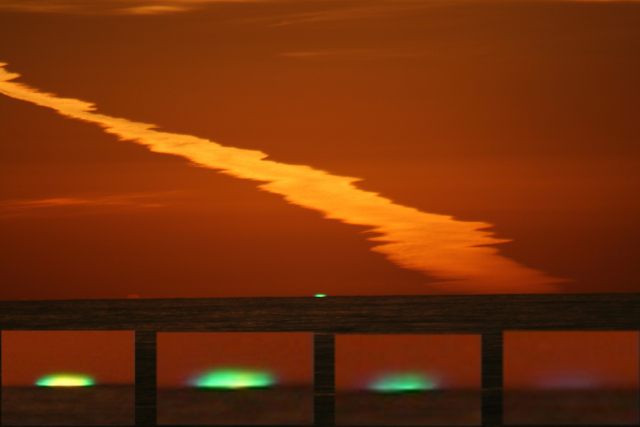
\includegraphics[width=\linewidth]{PP-N211.jpeg}
  \caption{Зелёный луч}
  \label{fig:pp-n211}
  \scriptsize
  \centering{}Источник: \url{https://news-ru.gismeteo.st/2023/07/Inferior_Mirage_green_flash-640x427.jpg}
\end{figure}

\p{212} Преобладание зеленоватых оттенков во время вечерней зари
указывает на длительную сухую ясную погоду.

\p{213}. Светлая серебристая полоска без всяких резких границ, долго
заметная у горизонта при безоблачном небе после захода солнца,
предвещает продолжительную тихую антициклональную погоду.

\p{214} Нежное розовое освещение неподвижных перистых облаков во время
захода солнца при отсутствии других облаков "--- надёжный признак
установившейся антициклональной погоды.

\p{215.} Преобладание в вечерней заре ярко красной окраски, которая
долго удерживается при дальнейшем опускании солнца за горизонт, служит
признаком приближения тёплого фронта или фронта окклюзии тёплого типа,
надо ожидать продолжительную ненастную, ветреную погоду.

\p{216} Нежно розовая заря в виде круга над зашедшим за горизонт солнцем
"--- хорошая устойчивая погода. Если окраска круга становится розово
красной, возможны осадки и усиление ветра. Расцветка зари тесно
связана с природой воздушной массы.

\subsubsection{Заход Солнца}

Так как циклоны движутся преимущественно от западных румбов, то
признаком приближения циклона обычно служит появление облаков на
западной половине небосвода. Если это происходит вечером, то солнце
заходит в облака.

\p{217} Если солнце заходит за низкое сплошное облако, выделяющееся
резко на фоне зеленоватого или желтоватого неба, то это признак
предстоящей хорошей (сухой, тихой и ясной) погоды.

\p{218} Если солнце заходит при сплошной низкой облачности и если на
горизонте и над облачностью наблюдаются слои перистых или
перисто-слоистых облаков, то выпадут осадки, наступит ветреная
циклональная погода в ближайшие 6--12~ч.

\p{219} Заход солнца за тёмные плотные облака с красной окраской по
краям предвещает циклональную погоду.

\p{220} Если после захода солнца на востоке отчётливо виден тёмный
постепенно распространяющийся вверх конус с широкой размытой оранжевой
каймой "--- тень земли (\rris{pp-n220}, то со стороны захода солнца
приближается циклон.

\begin{figure}[htb]
  \centering{}
  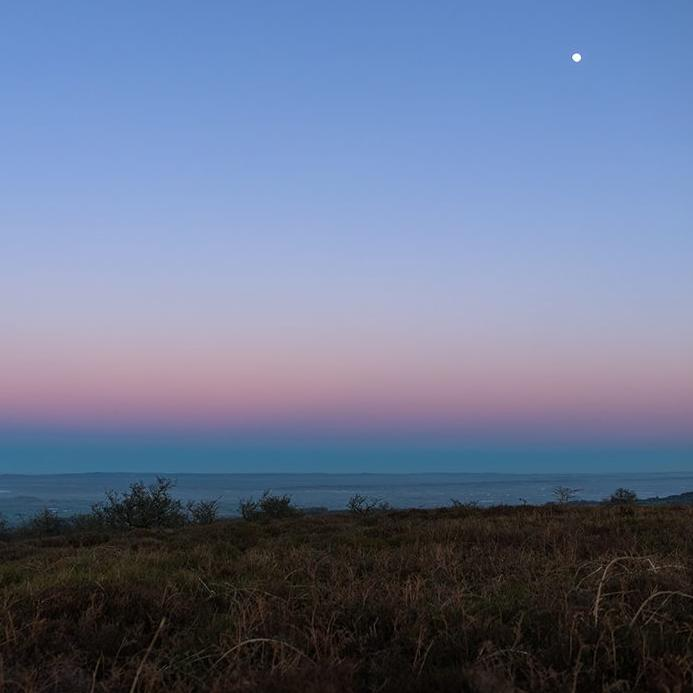
\includegraphics[width=\linewidth]{PP-N220.jpeg}
  \caption{Тень земли}
  \label{fig:pp-n220}
  \scriptsize
  \centering{}Источник: \url{https://facts.museum/3850}
\end{figure}

\p{221} Тень земли на востоке после захода солнца—серо-сизая, без цветной
окраски края или с бледно-розовой окраской — признак сохранения
антициклональной погоды.

\subsubsection{Иззаоблачное сияние}

Так называют пучок отдельных светлых лучей или полос, выходящих из-за
облаков, закрывающих солнце. Лучи солнца проходят через просветы между
облаками, освещают водяные капельки, парящие в воздухе во взвешенном
состоянии, образуя светящиеся полосы и снопы (лучи Будды). Поскольку
это сияние наблюдается благодаря присутствию в воздухе большого
количества мелких водяных капель, оно предвещает дождливую, ветреную
циклональную погоду.

\p{222} Сияние, выходящее из-за тёмного облака, за которым находится
солнце "--- признак наступления в ближайшие 3--6~ч ветреной погоды с
дождём.

\p{223} Сияние из-за облаков жёлтого цвета, наблюдаемое
непосредственно после прошедшего дождя, предвещает скорое
возобновление дождя и усиление ветра.

\subsubsection{Окраска небесных светил}

\p{224} Красный цвет солнца, луны и других небесных светил указывает
на большую влажность\index{влажность воздуха} в атмосфере, т.\=,е. установление в ближайшие
6--10~ч циклональной погоды с сильным ветром и осадками.

\p{225} Красноватый цвет затемнённого диска солнца вместе с
голубоватой окраской отдалённых предметов (гор и т.\=,п.) "--- признак
распространения запылённого тропического воздуха, нужно ожидать
скорого значительного повышения температуры.

\subsubsection{Форма небосвода}

Наблюдая небосвод с открытого места (например, в море), можно
заметить, что он имеет форму полушария, сплюснутого по
вертикали. Часто кажется, что расстояние от наблюдателя до горизонта в
три четыре раза больше, чем до зенита. Объясняется это тем, что при
взгляде вверх без откидывания головы назад предметы представляются
укороченными по сравнению с теми, которые находятся в горизонтальном
направлении.  Например, поваленные столбы или деревья кажутся длиннее
стоящих. По горизонтали действует атмосферная перспектива: окутанные
дымкой предметы кажутся более отдалёнными. Кажущаяся сплюснутость
небосвода изменяется в зависимости от условии погоды: её увеличивают
прозрачность и высокая влажность\index{влажность воздуха}.

\p{226} Сплюснутый, низкий небосвод наблюдается перед циклональной
погодой.

\p{227} Высокий небосвод наблюдается в центральных районах
антициклонов; можно ожидать, что хорошая погода антициклонального
характера сохранится в течение 12~ч и более.

\subsubsection{Гало}

Гало "--- оптическое явление в виде световых кругов вокруг Солнца и
Луны, иногда ложных солнц, световых столбов и крестов. Чаще всего гало
появляется в виде кругов с телесным углом при глазе наблюдателя 44\gr.

Внутренняя сторона кольца, обращённая к солнцу или луне, наиболее
яркая и окрашена в красноватый цвет. К внешней стороне круга окраска
переходит в желтоватую, зеленоватую и сине-фиолетовую. Часто бывает
виден не полный круг, а лишь его части, особенно верхняя. Иногда
заметны светлые дуги, которые касаются верхней или нижней части
круга. Редко наблюдается бесцветный круг, проходящий через диск Солнца
или Луны параллельно горизонту.

В точках пересечения горизонтального круга с гало часто видны
блестящие и яркие пятна, называемые ложными солнцами (паргелий). Гало
появляется тогда, когда между наблюдателем и солнцем или луной имеются
тонкие облака верхнего яруса (перисто-слоистые, перистые,
перисто-кучевые) или когда ледяные кристаллы, имеющие правильную
форму, главным образом в виде призм, взвешены в воздухе как отдельные
элементы.

Нередко гало наблюдается в виде вертикального столба. Чаще всего этот
столб виден, когда солнце или луна расположены вблизи горизонта, выше
или ниже его. Образование таких столбов объясняется отражением лучей
от горизонтальных граней взвешенных в воздухе ледяных кристаллов. При
сильных морозах по обе стороны солнца иногда видны два световых
столба, представляющих собой части дуги гало, когда весь круг не
виден.

Иногда столбы около солнца пересекаются с горизонтальным кругом. При
этом пересечении могут образовываться световые кресты. Разнообразие
явления гало (\rris{pp14}) объясняется многочисленными формами ледяных
кристаллов и различием расположения их в пространстве. Эти
обстоятельства создают разные условия преломления лучей света,
проходящих через кристаллик льда.

\begin{figure}[htb]
  \centering{}
  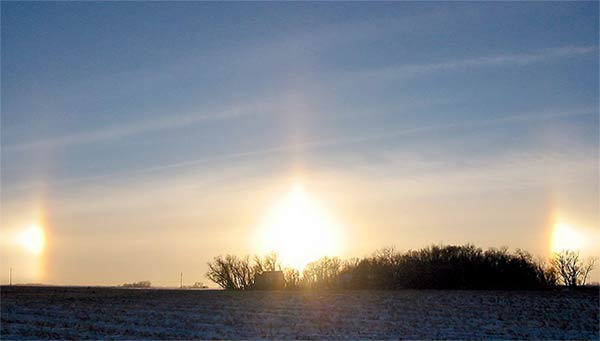
\includegraphics[width=\linewidth]{PP-14.jpeg}
  \caption{Гало с ложными солнцами}
  \label{fig:pp14}
  \small
  \centering{}фото: Erik Axdahi
\end{figure}

\p{228} Появление полного светового радужного круга по телесному углу
44\gr около солнца или луны, возникающего при наличии тонкой пелены
перисто-слоистых облаков (\rris{pp15}), иногда едва заметной для
глаза, "--- признак приближения циклона, тёплого фронта или фронта
окклюзии тёплого типа; надо ожидать наступления ветреной погоды в
ближайшие 12--20~ч. При этом яркость светового круга постепенно
усиливается и начинает ослабевать лишь при сильном уплотнении перистых
облаков

\begin{figure}[htb]
  \centering{}
  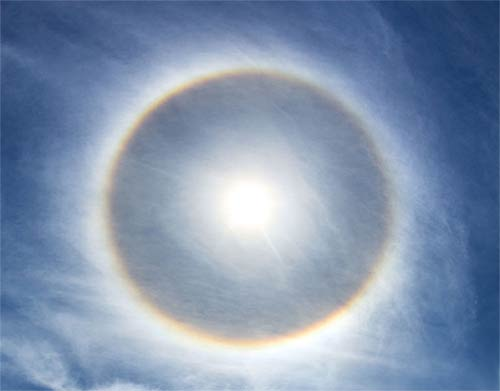
\includegraphics[width=\linewidth]{PP-15.jpeg}
  \caption{Гало}
  \label{fig:pp15}
  \small
  \centering{}фото: Anton Yankovyi
\end{figure}

\p{229} Белые световые круги (без радужной окраски) вокруг светил,
столбы и ложные солнца указывают на сохранение тихой, ясной
антициклональной погоды, зимой "--- на сильные морозы, которые продержатся
12~ч и более.

\p{230} Световые круги около солнца или луны, появляющиеся о виде
неполного кольца, наблюдаются в неустойчивых воздушных массах, в
периферийных районах антициклонов, в тыловой части циклона; при этом
возможна переменная погода с проходящими ливневыми осадками и сильными
ветрами.

\p{231} Белые световые круги большого диаметра, видимые под углом 92\gr,
около солнца или луны, появляющиеся зимой "--- признак того, что здесь
находятся центральные районы мощного антициклона или отрога высокого
давления; можно ожидать устойчивую погоду со слабыми ветрами, штилями
и с сильными морозами.

\subsubsection{Венцы}

Венцы "--- радужные кольца по телесному углу от глаза наблюдателя
2--10\gr, окаймляющие солнце, луну, яркие звезды и другие источники
света. Венцы около луны видны простым глазом, а около солнца "--- через
тёмное стекло или по отражению светила на спокойной воде. Внутренняя
часть венца, непосредственно примыкающая к светилу, имеет голубоватую
или голубовато-белую окраску, за ней располагается желтоватое кольцо,
переходящее снаружи в красное.

Эти радужные кольца образуют так называемый ореол. Бывает, что ореол
окружён ещё одним, двумя или тремя менее яркими радужными кольцами с
таким же расположением цветов. Возникают венцы в результате
дифракции\footnote{Дифракция света "--- отклонение светового луча от
  прямолинейного пути при прохождении через очень малые отверстия,
  величина которых близка к длине световых волн,
  т.\=,е. 0,4--0,7~мкм.} света.

В тонких слоях облаков луч света проходит через водяные капли или
кристаллы льда. Различного цвета лучи, составляющие белый свет, при
прохождении через малые отверстия отклоняются и освещают пространство,
лежащее за ними. Лучи разного цвета (длины волны) отклоняется
по-разному, поэтому венцы имеют радужную окраску.

Для образования венцов нужно, чтобы размеры капель или кристаллов,
составляющих облако, были приблизительно одинаковы, в противном случае
вокруг солнца или луны вместо венцов образуется размытое белое
пятно. Размеры венцов зависят от размеров капелек воды или
кристалликов льда, образующих облако: чем они крупнее, тем меньше
размеры венцов. Поэтому по изменению с течением времени диаметра венца
можно судить об изменении размера частиц в облаке. Увеличение диаметра
указывает на уменьшение частиц, а следовательно, на уменьшение влаги в
атмосфере; наоборот, уменьшение диаметра венца свидетельствует о
возрастании размера частиц, об увеличении влаги в атмосфере.

С венцами связана и так называемая иризация облаков. Это явление
состоит в том, что отдельные части облаков, обычно их края,
приобретают радужную окраску, чаще всего красного и зелёного
цветов. Окрашенные края являются частью венца с большим радиусом.

\p{232} Радужные венцы вокруг солнца и луны с неяркой окраской,
постепенно уменьшающиеся в размерах "--- признак приближения тёплого
фронта или фронта окклюзии тёплого типа; нужно ожидать наступления
продолжительной ненастной ветреной погоды. И наоборот, венцы вокруг
солнца или луны с яркой радужной окраской, увеличивающиеся в размерах,
"--- признак наступления ясной и тихой антициклональной погоды.

\p{233} Уменьшение диаметра венца "--- признак ненастной погоды,
увеличение "--- признак прояснения и установления хорошей погоды.

\p{234} Появление малого радужного венца, рельефно выделяющегося вокруг
луны и почти прилегающего к ней "--- признак наступления ветреной с
осадками циклональной погоды на следующий день или через два дня.

\p{235} Иризация в высококучевых облаках при их прохождении на
сравнительно небольшом расстоянии от солнца "--- признак приближения
холодного фронта или фронта окклюзии холодного типа; следует ожидать
непродолжительной ненастной погоды со шквалами\index{ветер!шквал}\index{шквал}, ливнями, грозами
(летом), которая сменится похолоданием.

\p{236} Иризация с неяркой радужной окраской на тающих краях кучевых
облаков при прохождении их вблизи солнца "--- признак установления
антициклональной погоды с кучевой переменной облачностью.

\subsubsection{Мерцание звёзд}

Мерцание звёзд вызывается состоянием атмосферы, которая никогда не
бывает спокойной: движение и флуктуации плотности воздуха вызывают
преломление света точечных источников "--- звёзд "--- который при этом
отклоняется и для наблюдателя меняет яркость. Свет с разной длиной
волны преломляется и рассеивается неодинаково, в связи с чем мерцание
звёзд может иметь разную окраску. Мерцание становится заметнее по мере
приближения звезды к горизонту, потому что свет здесь проходит гораздо
большую толщу атмосферы. Планеты почти не мерцают, так как они видны
не как точечные источники, а маленькие диски. Мерцание их точек
накладывается друг от друга, и средняя сила света остаётся одинаковой.

Мерцание звёзд усиливается при понижении температуры, увеличении
влажности\index{влажность воздуха} и усилении ветра на различных высотах. Следовательно,
интенсивное мерцание звёзд говорит о большой влажности воздуха, о
неспокойном состоянии атмосферы в верхних слоях, если даже внизу
наблюдается штиль.

\p{237} Сильное мерцание звёзд (иногда и дрожание) с преобладанием
синего или красного цвета "--- признак приближения циклона и установления
влажной\index{влажность воздуха} ветреной погоды.

\p{238} Интенсивное мерцание звёзд к утру на темпом фоне неба "---
признак скорого дождя.

\p{239} Мерцание звёзд с преобладанием зелёного цвета указывает на
малую влажность\index{влажность воздуха} в атмосфере "--- признак установления продолжительной
жаркой сухой погоды.

\subsubsection{Радуга}

В каплях дождя солнечные лучи преломляются и разлагается на
спектральные цвета, образуя радугу. Центр радуги расположен в точке
небосвода, прямо противоположной солнцу. Поэтому, когда солнце
находится на горизонте, радуга представляет собой дугу — половину
окружности. Когда солнце поднимается над горизонтом, радуга опускается
и уменьшается в размерах. При высоте солнца над горизонтом 42\gr радуга
не видна. Число и яркость цветов, а также ширина радуги зависят от
размера капель, образующих её, и от запаса влаги в атмосфере. Чем
крупнее капли, тем ярче выражены цвета радуги и тем она уже.

При небольших каплях, например в тумане, образуется широкая и белая
радуга, она бывает слабо окрашена по краям. Иногда такую радугу можно
увидеть во время дождя ночью, при лунном свете.

Радуга утром и вечером имеет разное значение. Объясняется это тем, что
облачность и осадки чаще всего движутся с запада на восток и,
следовательно, если радуга наблюдается утром, т.\=,е. в западной части
неба, то к вечеру дождевые облака оттуда могут прийти к месту
наблюдения. Если же радуга наблюдается вечером, т.\=,е. в восточной
стороне неба, это значит, что дождевые облака уходят от места
наблюдения дальше на восток.

\begin{figure}[htb]
  \centering{}
  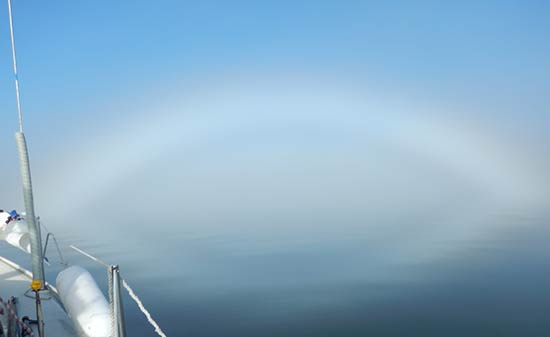
\includegraphics[width=\linewidth]{PP-15a.jpeg}
  \caption{Белая радуга}
  \label{fig:pp15a}
  \small
  \centering{}фото: Г.Шмерлинг
\end{figure}

\p{240} Радуга утром или перед полуднем предвещает ливневый дождь,
сильный ветер со шквалами\index{ветер!шквал}\index{шквал} и часто с грозой.

\p{241} Радуга после полудня или вечером "--- признак прекращения дождя и
установления ясной тихой погоды.

\p{242} Переход цветной радуги в белую указывает на уменьшение
размеров капель и на скорое прекращение дождя.

\p{243} Переход белой радуги в цветную "--- признак скорого дождя.

\p{244} Радуга с наветренной стороны "--- день будет дождливым.

\p{245} Радуга с подветренной стороны "--- погода скоро прояснится, дождь прекратится.

\p{246} Усиление красного цвета в радуге "--- к дождливой погоде.

\p{247} Резкое выделение зелёного цвета в вечерней радуге "--- признак
установления сухой, ясной маловетреной погоды.

\subsubsection{Рефракция, деформации у горизонта, миражи}

\begin{figure}[htb]
  \centering{}
  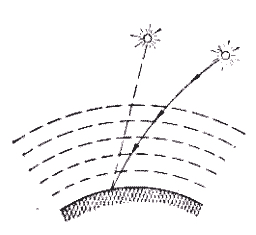
\includegraphics[width=\linewidth]{PP-16.jpeg}
  \caption{Рефракция}
  \label{fig:pp16}
  \small
  \centering{}
\end{figure}

Рефракция возникает из-за преломления лучей света в атмосфере,
обусловленного неодинаковым распределением плотности воздуха. Чем выше
плотность среды, тем меньше в ней скорость света; в результате фронт
световой волны поворачивает в ту сторону, где выше плотность. Иначе
говоря, так же ведёт себя луч света, пронизывающий атмосферу,
плотность которой уменьшается с высотой (\rris{pp16}), а также зависит от
температуры.

Глаз человека не учитывает рефракцию: мы видим предметы по тому
направлению, по которому пришли лучи. Поэтому при нормальной рефракции
светило или далёкий предмет кажется лежащим выше своего
действительного положения. Угол рефракции зависит от высоты светила
над горизонтом, около которого достигает 0,5\gr. Таким образом, солнце и
другие светила видны на своих местах только тогда, когда они находятся
в зените, в других случаях они кажутся несколько приподнятыми. При
заходе мы наблюдаем светила над горизонтом, когда на самом деле они
уже скрылось за него. Поэтому в умеренных широтах фактическая
продолжительность дня увеличивается на 8--13~мин, а в высоких широтах
полярная ночь сокращается почти на две недели против теоретической.

Рефракция оказывает влияние на форму дисков солнца и луны у
горизонта. У линии горизонта разность углов рефракции для нижнего и
верхнего краёв светила настолько велика, что нижний край оказывается
относительно более приподнятым, чем верхний: диск солнца или луны
кажется сплюснутым.

Рефракция проявляется и для земных объектов, например, линия берега с
моря кажется выше, чем на самом деле. Из-за рефракции предметы, в
действительности находящиеся уже за горизонтом, оказываются ещё
видимы.

Тонкий слой лёгкого тумана на горизонте при восходе или заходе солнца
и луны, особенно при ясной, тёплой и тихой погоде, вызывает вследствие
больших изменений плотности в самых нижних слоях атмосферы причудливые
искажения контуров диска солнца или луны. Иногда наблюдается появление
второго солнца на некотором расстоянии от первого.

Мираж "--- мнимое изображение отдалённого объекта, который при этом
кажется увеличенным или уменьшенным, перевёрнутым или искажённым "--- в
зависимости от отклонения лучей света при рефракции. Одновременно
объект может быть виден и в его истинном положении.

Миражи часто наблюдается в степях и пустынях жарких стран и на океанах
и морях, особенно в высоких широтах. Нередко можно видеть несколько
изображений одного и того же судна, причём некоторые из них обращены
мачтами вниз. Иногда же очертания берегов и других предметов так
сильно искажаются, что даже при хорошем знании местности бывает трудно
её опознать.

Миражи возникают при ясной погоде и высоком атмосферное давлении,
когда в нижних слоях воздуха плотность изменяется с высотой не плавно,
а скачкообразно. В этом случае лучи света, идущие к наблюдателю от
различных предметов, испытывают полное внутреннее отражение на границе
слоев воздуха с различными плотностями. Иначе говоря, причина
возникновения миража — необычная, повышенная рефракция света,
образующаяся при резком изменении плотности воздуха по вертикали в
нижнем слое атмосферы.

Например, если тёплый воздух распространяется над холодной водой и
особенно над ледяным или снежным покровом, то у подстилающей
поверхности температура низкая, а с высотой будет заметно
увеличиваться, уменьшая плотность. Лучи от далёких объектов будут идти
по выпуклой вверх кривой, и в результате эти объекты покажутся
наблюдателю приподнятыми. Известны случаи, когда с побережья Крыма был
виден берег Турции, находящийся на расстоянии 400~км. Такое явление
называется верхним миражем (\rris{pp17})

\begin{figure}[htb]
  \centering{}
  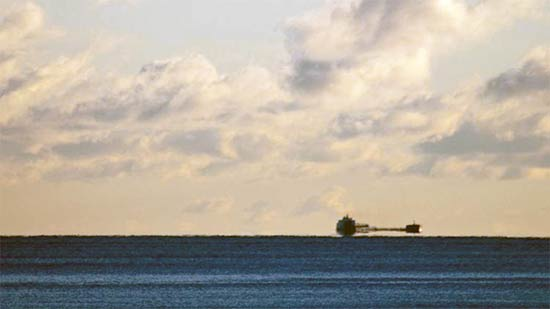
\includegraphics[width=\linewidth]{PP-17.jpeg}
  \caption{Верхний мираж}
  \label{fig:pp17}
  \small
  \centering{}
\end{figure}

Когда над тёплой поверхностью, в том числе сравнительно тёплым морем,
находится более холодный воздух, нижние слои воздуха менее плотные,
чем находящиеся над ними. В этом случае траектория светового луча
обращена выпуклостью вниз, и отдалённые предметы кажутся
перевёрнутыми. Это явление называется нижним миражем (\rris{pp18}).

\begin{figure}[htb]
  \centering{}
  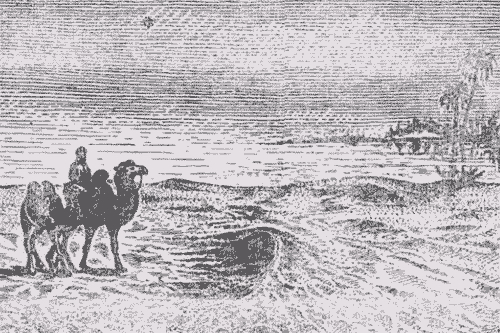
\includegraphics[width=\linewidth]{PP-18.jpeg}
  \caption{Нижний мираж в пустыне}
  \label{fig:pp18}
  \small
  \centering{}
\end{figure}

Вызывающее миражи сильное охлаждение либо нагревание земной
поверхности может происходить при тихой ясной погоде. Кратковременные
миражи довольно часто наблюдаются в прибрежной зоне морей и океанов и
указывают на устойчивую антициклональную погоду. Нижний отчётливо
видимый мираж, возникающий после тихой жаркой погоды при сильном
нагреве приземного слоя воздуха обусловливает неустойчивое состояние
атмосферы, которое может в любое время привести к ненастной ветреной
погоде. Признаками наступления миража и сильной рефракции на море
может служить кажущееся дрожание горизонта, а также наличие мглы на
горизонте.

\p{248} Деформация формы диска солнца луны и других светил у горизонта
при восходе или заходе предвещает тихую, ясную погоду без осадков.

\p{249} Устойчивый верхний мираж — признак наступления ненастной
циклональной погоды.

\p{250} Длительный нижний мираж указывает на ненастную погоду.

\p{251} Кратковременный мираж на берегу моря "--- признак устойчивой
антициклональной погоды.

\subsubsection{Сумерки}

Сумерками называется переходное время от дневного свет к темноте
вечером или от темноты к свету утром. Различают сумерки гражданские и
астрономические. Гражданские сумерки "--- это промежуток времени, за
которое солнце прячется за горизонт до угла 6--8\gr над ним. В этот
период на открытом воздухе можно читать и писать без искусственного
освещения.

Астрономические вечерние сумерки заканчиваются, когда солнце
опускается за горизонт и наступает полная темнота. Продолжительность
сумерек зависит от широты места, времени года и погоды. Наиболее
короткие сумерки наблюдаются на экваторе, где через 24~мин после
захода солнца наступает темнота. С широтой продолжительность сумерек
значительно увеличивается.

В Арктике и Антарктике при переходе от полярного дня к полярной ночи
или наоборот сумерки могут продолжаться несколько суток. При большой
влажности\index{влажность воздуха} и запылённости воздуха продолжительность сумерек в среднем
больше, чем при менее влажном и чистом. Облака тоже влияют на
продолжительность сумерек: при наличии облаков верхнего яруса сумерки
удлиняются, а при облаках среднего и нижнего ярусов "--- укорачиваются.

\p{252} Короткие сумерки свидетельствуют о большой прозрачности
атмосферы (о небольшой влажности\index{влажность воздуха} и малой запылённости воздуха) "--- можно
ожидать наступления или сохранения ясной, тихой антициклональной
погоды.

253. Продолжительные сумерки свидетельствуют о большой влажности\index{влажность воздуха} и
запылённости атмосферы "--- признак приближения циклона и наступления
влажной ветреной погоды.

\subsection{Акустические (звуковые) явления}

\subsubsection{Слышимость}

Слышимость звука зависит от плотности, влажности\index{влажность воздуха}, температуры воздуха
и ветра. Во влажном воздухе слышимость звука резко возрастает, в сухом
"--- уменьшается. Перед ветреной погодой звук слышен неровно. Если
хорошая или плохая слышимость звука не обусловлена попутным или
встречным ветром, то признаки погоды следующие.

\p{254} Хорошая слышимость отдалённых (слабых) звуков объясняется
повышенной влажностью\index{влажность воздуха} воздуха и служит признаком наступления ненастной
погоды с осадками.

\p{255} Плохая слышимость звука указывает на улучшение погоды.

\subsubsection{Гром}

Гром распространяется, как и всякий другой звук, со скоростью около
330\speedms. Определив время, прошедшее от разряда молнии до момента,
когда будет слышен гром, можно легко вычислить расстояние, отделяющее
наблюдателя от молнии, а следовательно, и от кучево-дождевого (часто
со шквалами\index{ветер!шквал}\index{шквал}) облака. При слабом ветре и штиле гром слышен на
расстоянии 25--30~км и проходит его за 70--90~сек после молнии.

\p{256} Утренний гром "--- признак выпадения дождя к вечеру.

\p{257} Если летом в прохладную дождливую погоду гром слышен утром, то
надо ожидать сохранения на продолжительное время данной погоды, часто
с дальнейшим понижением температуры.

\subsection{Волны на море}\label{sec:waves_on_sea}

Наблюдения показывают, что в области шторма из-за непостоянства ветра
по силе и направлению на поверхности моря зарождаются волны различной
высоты, длины и периодов. В начале шторма, когда ветер ещё слаб,
возникают короткие волны с малым периодом. Скорость распространения
волн пропорциональна их длине и периоду. Волны зыби имеют большие
длину и период, чем ветровые волны, поэтому и распространяются они
быстрее. Поэтому распространяющиеся впереди циклона длинные волны,
приходящие к месту наблюдения в маловетреную и штилевую погоду в виде
зыби и мёртвой зыби, служат признаками ухудшения погоды.

Обычно через 6--12~ч после появления зыби и мёртвой зыби приходит и
полоса шторма.

С помощью специальных наблюдений удалось установить, что впереди
фронта видимых длинных волн распространяются мало заметные и не
заметные простому глазу очень низкие (30--40~см) и более длинные (700~м
и больше) волны. Они получили название предшественниц зыби. Их период
около 30~с, тогда как период обычной зыби равен в среднем 10~с.
Вследствие этих различий более длинные волны распространяются со
скоростью около 1100~миль в сутки, в то время как обычная зыбь
движется со скоростью 400~миль в сутки.

\p{258} Зыбь, идущая от другого направления, чем ветровая волна или
волны, наблюдаемые при штиле, —признак приближающегося шторма, следует
внимательно следить за остальными признаками, указывающими на это.

\p{259} Если зыбь начинает идти не по ветру и все усиливается, то
циклон приближается своим тёплым фронтом. Если зыбь не усиливается, а,
наоборот, со временем слабеет или меняет направление, то это указывает
на то, что циклон (шторм, ураган) проходит стороной.

\p{260} Появление в данном месте пологих волн небольшой высоты (30--40~см)
и большой длины указывает на приближение большой зыби и шторма в
ближайшие 1--2~суток.

\p{261} Сильный прибой у берегов при тихой погоде служит признаком
циклона (или урагана), проходящего на большом расстоянии.

\p{262} Если при штиле море начинает покрываться короткими волнами
"--- это признак скорого наступления свежего ветра.

\subsection{Поведение живых существ}

Многие животные (птицы, рыбы, морские звери, насекомые и др.) и
растения гораздо раньше приборов реагируют на намечающиеся резкие
изменения погоды. Например, рачки-бокоплавы задолго до шторма, когда
барометр\index{барометр} не показывает ещё никаких признаков ухудшения погоды,
выбираются на берег подальше от воды. По той же причине рыбы и медузы
уходят перед штормом вглубь моря, а пингвины ложатся на снег и
вытягивают клювы в направлении шторма. Чайки и другие морские птицы
перед наступлением шторма летят к берегу.

\p{263} Если чайки и другие морские птицы вылетают рано утром и
удаляются далеко в море, то штормового ветра можно не ожидать до
вечера.

\p{264} Если птицы при слабом ветре держатся у берега и не улетают далеко
в море, надо ожидать усиления ветра.

\p{265} Массовое возвращение птиц с моря к берегу указывает на скорое
приближение шторма

\p{266} Дельфины собираются в косяки, стаи больше обычного резвятся
"--- признак приближения шторма.

\p{267} Касатки, высоко прыгая из воды, стремительно уходят от берегов
в открытый океан, киты отходят от кромки льда "--- признак приближения
шторма в ближайшие 12--14~ч.

\p{268} Если медузы, живущие колониями в тропических и тёплых морях,
плавают в большом количестве на поверхности моря "--- признак, что
маловетреная ясная антициклональная погода на ближайшие 12--24~ч
сохранится. При наступлении циклона и ухудшении погоды медузы уходят
под воду на глубину.

\p{269} Если рачки, живущие в прибрежной зоне, выходят на берег, а рыбы и
медузы уходят в глубь моря, надо ожидать наступления циклона, шторма.

\p{270} Появление на южных берегах и островах Балтийского моря поздней
осенью больших стаи птиц предсказывает раннюю и суровую зиму.

\subsection{Радиопередачи}

Помехи, которые мы часто слышим в виде треска, шороха и щелчков,
обычно называют <<атмосфериками>>. При их изучении выяснилось, то трески
и щелчки появляются, когда между передающим и приёмным пунктами
наблюдаются ливневые осадки с грозами, шквалами\index{ветер!шквал}\index{шквал}, а шорохи "---
сплошной фон осадков без гроз.

Следовательно, прослушав несколько радиостанций, можно приблизительно
определить погоду большого района. Отмечая направление источника
тресков и других атмосфериков из нескольких пунктов радиопередачи
можно определить район грозовой деятельности, штормов и
циклонов. Кроме того, районы осадков, находящиеся на пути
распространения радиоволн между передатчиком и приёмником, значительно
ослабляют слышимость радиостанции. Но если передающие и принимающий
пункты находятся в районе осадков, связанных с одним фронтом,
слышимость резко возрастёт. По интенсивности и характеру приёма
атмосфериков можно не только обнаружить положение атмосферных фронтов,
но и их трансформацию. Если сравнивать, например через 2--3~ч,
слышимые при приёме атмосферные помехи, можно отметить их усиление или
ослабление и как часто помехи повторяются.

Наблюдениями установлено, что области циклонов характеризуются
повышенными атмосферными радиопомехами. Направление, по которому эти
помехи обнаруживаются, наиболее интенсивно указывает на центр
циклона. Направление помех можно определить путём радиопеленгования.

Таким образом, атмосферики являются своеобразными местными признаками
погоды.

\p{271} Если при прослушивании радиостанции слышен треск, то это
означает, что между передатчиком и приёмником на близком расстоянии от
пункта приёма проходит холодный фронт. Чем ближе фронт к пункту
приёма, тем сильнее и чаще трески

\p{272} Если при радиоприёме слышны щелчки, то это означает, что между
передатчиком и приёмником очень далеко от пункта приёма проходит
холодный фронт

\p{273} Если при радиоприёме слышны шорохи, то на пути радиоволн между
передатчиком и приёмником близко проходит тёплый фронт.

\p{274} Если при приёме слышен сплошной фон т.\=,е. шум одного тона то
между передающей станцией и приёмником находится тёплый фронт.

\p{275} Усиление слышимости атмосферных радиопомех "--- признак
обострения, усиления фронта.

\p{276} Ослабление слышимости атмосферных радиопомех "--- признак
ослабления (размывание) фронта.

\p{277} Ослабление или полное прекращение приёма коротко волновых
станции "--- признак ненастной циклональной погоды между станциями и
пунктом приёма.

\subsection{Опасные для мореплавания явления погоды}

\subsubsection{Тропические циклоны}

В тропической зоне в широтах от 5~до 25\gr обоих полушарий наблюдаются
циклоны, обладающие огромной разрушительной силой. Тропические циклоны
небольшие по размерам, в среднем 100--200~миль в диаметре, с очень
низким давлением в центре (глубокие циклоны). Они сопровождаются
мощной, спускающейся до земли, грозовой облачностью, ураганными
ветрами, сильными ливнями, огромными океанскими волнами. Даже самым
крупным современным судам очень трудно бороться с ураганом, и часто
эта борьба заканчивается гибелью судна. Давление в центральной области
тропического циклона в среднем бывает 960--970~мбар, но иногда 900~мбар
и ниже.

Разница в давлении между центром и периферией тропических циклонов на
1\gr расстояния (111~км), так называемая величина барического градиента\index{барический градиент},
составляет 30--40, а иногда и более 100~мбар. тогда как в обычных
циклонах она, как правило, не превышает 20--25~мбар. По этой причине
скорость ветра в тропических циклонах обычно достигает 50--60\speedms и
более.

Возникают тропические циклоны только над океанами и морями, согласно
одной из теорий, от восходящих токов тёплого и влажного\index{влажность воздуха} воздуха,
которые приводят к выделению огромных количеств тепла в результате
конденсации водяных паров. Другая теория объясняет это явление
взаимодействием воздушных масс северного и южного полушарий в зоне
сходимости пассатов\index{пассат}. Ясно, что тропические циклоны возникают в таких
океанических районах и в те сезоны года, когда температура поверхности
моря наибольшая и превышает 26--27\grC.

Не совсем ясна пока ещё структура тропических циклонов. В то время как
кругом бушуют ураганные ветры, сильнейшие ливни и грозы, в центре,
диаметром в среднем 10--15~миль, наблюдается область ясной штилевой
погоды "--- <<глаз бури>> Наиболее опасной является правая (по движению)
половина циклона в северном полушарии, в южном "--- левая. Здесь скорость
ветра нередко достигает 65\speedms, а скорость отдельных шквалистых\index{ветер!шквал}\index{шквал}
порывов 100\speedms и более.

Наиболее часто тропические циклоны в северном полушарии наблюдаются в
период с августа по сентябрь, а в южном полушарии в районе Тихого
океана "--- с января по июль, в Индийском океане "--- с ноября по апрель
Исключение составляет северная часть Индийского океана, где
тропические циклоны чаще встречаются с мая по декабрь.

Тропические циклоны, зарождающиеся на западе Тихого океана, называются
тайфунами, в Атлантическом океане "--- Антильскими ураганами, в северной
части Индийского океана "--- циклонами, в южной "--- орканами, у берегов
Австралии "--- вилли-вилли. В отличие от обычных циклонов, тропические
движутся с востока на запад, а некоторые, пересекая тропические
широты, меняют направление и идут в северном полушарии к
северо-востоку, а в южном "--- к юго-востоку Если с переходом в средние
широты тропический циклон встречает полярный фронт, он значительно
увеличивается в размерах и превращается в обычный глубокий циклон с
тёплым и холодным фронтом.

\begin{figure}[htb]
  \centering{}
  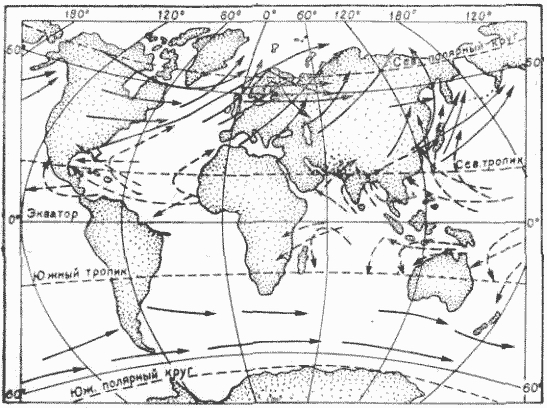
\includegraphics[width=\linewidth]{PP-22.jpeg}
  \caption{Основные районы зарождения и пути движения циклонов}
  \label{fig:pp22}
  \small
  \centering{}
  тропические циклоны "--- пунктирные линии, циклоны умеренных широт "--- сплошные
\end{figure}

В среднем за год в Тихом океане наблюдается около 20--23 циклонов, в
Атлантическом 12--13, в Индийском около 15. Пути тропических циклонов,
за редким исключением, постоянны. Скорость движения тропических
циклонов вначале бывает небольшой, но у хорошо развитых достигает
15--20~уз и более. Продолжительность существования тропических циклонов
составляет в среднем 8--10~суток.

При прохождении в море тропического циклона появляется характерный
нарастающий шум. Чёрные или красные клочья разорванных облаков быстро
проносятся по небу. С большой скоростью надвигается огромное чёрное
облако, закрывая все небо. Ветер усиливается, становится порывистым,
начинают беспрерывно налетать шквалы\index{ветер!шквал}\index{шквал}. Гремит не переставая большой
силы гром, огромные ослепительные молнии часто пронизывают наступивший
мрак.

Очень сильный ветер создаёт гигантские волны, обладающие огромной
силой. Потоки дождевой воды смешиваются в воздухе с брызгами и пеной
от волн, видимость уменьшается до нескольких метров. Такое состояние
погоды и моря может длиться много часов. Когда проходит центр
тропического циклона (<<глаз бури>>), минут на 20--30 ветер стихает до
штиля, проясняется, можно видеть голубое или звёздное небо, но
волнение моря не уменьшается Волны здесь сходятся от всех направлении
и создают чрезвычайно крутую и беспорядочную, очень опасную для судов
толчею (стоячие волны длиной около 40~м). По мере удаления от центра
циклона волнение принимает более упорядоченный, регулярный
характер. После прохождения <<глаза бури>> барометр\index{барометр} делает быстрый
скачок вверх, и от противоположного румба снова налетает шквал\index{ветер!шквал}\index{шквал}
ураганной силы.

Общий характер погоды становится таким же, как и до прохождения центра
циклона. Иногда в тропическом циклоне наблюдаются смерчи\index{смерч}\index{ветер!смерч} "--- небольшие
по размерам вихри диаметром в несколько сот метров при скорости
перемещения до 20--25~уз. Ветер в таком вихре имеет колоссальную
скорость 200--250\speedms. Отличительная особенность смерчей "---
воронкообразное опускание облачности с длинным отростком вниз в виде
хобота, конец которого иногда касается воды. Смерчи обладают огромной
разрушительной силой.

Опасность тропических циклонов для мореплавания ещё усугубляется и
тем, что из-за относительно малых размеров они не всегда могут быть
обнаружены синоптиками службы погоды. По этой причине суда,
находящиеся в море, не могут своевременно получить предупреждения о
зарождении и пути перемещения урагана. Поэтому особо важное значение
имеют местные признаки приближающихся тропических циклонов.

При передаче по радио сведений о тропических циклонах им присваиваются
женские имена Вера, Диана, Нэнси, Шарлотта и др. В старину тропическим
циклонам давали имена кораблей, которые их обнаружили.

\p{278} Как уже было сказано в разделе <<Волны на море>>
(см.~\ref{sec:waves_on_sea}, стр.~\pageref{sec:waves_on_sea}), по
направлению зыби можно судить о положении центра циклона, а по
изменению её направления "--- о направлении движения
циклона. Появление зыби, идущей не от того направления, от которого
дует или дул ранее ветер "--- признак приближения тропического
циклона.

\p{279} При приближении тропического циклона атмосферное давление
резко изменяется, поэтому наблюдение за показаниями барометра\index{барометр} и
барографа\index{барограф} является одним из важных факторов своевременного обнаружения
и предсказания приближающегося тропического циклона. Атмосферное
давление на расстоянии 120--150~миль от центра тропического циклона
начинает постепенно падать, но ещё заметно сохраняется его суточный
ход.

Далее с приближением центра тропического циклона на расстояние
60--110~миль суточный ход давления полностью нарушается, давление
резко падает (на 13--20~мбар в час), падение давления прекращается лишь
при прохождении <<глаза бури>>. После прохождения центра тропического
циклона давление начинает повышаться вначале быстро, а затем, с
удалением центра "--- медленнее и наконец достигает нормального значения
для данного района.

\p{280} Приближению тропического циклона иногда на очень больших
расстояниях (до 1500~миль) предшествует появление перистых
нитеобразных облаков с загнутыми концами, которые лучше всего
наблюдаются при восходе или заходе солнца. Если эти облака кажутся
сходящимися в одной точке, то с большой вероятностью можно считать,
что на расстоянии около 500~миль от судна в районе сходимости этих
облаков расположен центр тропического циклона На расстоянии около 300~миль
от центра тропического циклона направление движения перистых
облаков часто совпадает с направлением движения циклона.

Перистые облака не всегда являются безусловным признаком приближения
тропического циклона, однако появление их не следует оставлять без
внимания. На расстоянии 500--600~миль от центра циклона обычно
наблюдаются перисто кучевые облака, а на расстоянии 200--250~миль "---
нагромождения мрачных мощных кучево-дождевых облаков, вид неба в этот
момент угрожающий. Появлению кучево-дождевых облаков часто
предшествует возникновение на горизонте небольшого, заметно
увеличивающегося и быстро движущегося тёмного облака "--- <<бычьего
глаза>>.

На расстоянии 200--250~миль от центра тропического циклона хорошим
признаком его приближения является появление разорванно-кучевых
облаков. Вначале это одиночные облака, но с приближением центра
циклона количество их увеличивается, они уплотняются и постепенно
переходят в дождевые. Одновременно проходят шквалы\index{ветер!шквал}\index{шквал} с ливнями.

Движение разорванно-кучевых облаков указывает на направление движения
центра тропического циклона. Если стать лицом навстречу движению этих
облаков, то центр тропического циклона будет расположен вправо от
судна. В 100--150~милях от центра тропического циклона начинается
сильный ливневый дождь, который хорошо просматривается на экране
судового радиолокатора.

В 10--15 милях от центра дождь прекращается, облака расходятся. После
прохождения центральной области тропического циклона облака снова
смыкаются и начинается ливневый дождь такой же силы, как и до
прохождения центра циклона, однако продолжительность дождя несколько
меньше. С удалением тропического циклона дождевые облака переходят в
кучевые, и дождь прекращается.

\p{281} При приближении тропического циклона, так же как и при
приближении обычного, иногда наблюдаются гало и венцы вокруг солнца и
луны.

\p{282} Багрово-красная окраска зари "--- признак приближения тропического
циклона. Причём вечерняя заря удерживается долгое время и остаётся до
конца красной, не переходя в жёлтый цвет. В то же время с
противоположной стороны хорошо видна тень земли, край которой имеет
оранжевую окраску. Такая заря может наблюдаться за 2--3~суток до
наступления циклона. Иногда тропическим циклонам предшествуют восходы
и за ходы солнца, при которых небо принимает огненный или
медно-красный цвет с разнообразными оттенками.

\p{283} За сутки и более до наступления тропического циклона
наблюдается ясное небо, штиль или слабый ветер, значительное повышение
температуры, абсолютной и относительной влажности\index{влажность воздуха} воздуха (ощущается
сильная духота) и нарушение их суточного хода, с начала наступления и
дальнейшего прохождения циклона наблюдается быстрое падение
температуры воздуха.

\p{284} Ночью со стороны приближающегося тропического циклона часто видны
сильные отблески молний (зарницы).

\p{285} При радиоприёме слышатся частые разряды или сплошной треск,
усиливающийся по мере приближения циклона.

\p{286} На экране радиолокатора появляются отдельные светлые пятна,
представляющие собой крупнокапельные скопления в атмосфере

\p{287} Направление ветра в различных частях тропического циклона
изменяется так же, как и в циклонах умеренных широт, отличаясь только
гораздо более быстрым переходом от одного румба к другому. Направление
ветра — хороший признак определения местонахождения центра
тропического циклона. По изменению направления ветра можно судить, в
какой половине циклона относительно его пути находится судно
(см.~\ref{sec:evasion_from_cyclones}).

\p{288} Увеличение скорости ветра "--- признак приближения тропического
циклона, но этот признак проявляется слишком поздно.

\subsubsection{Глубокие циклоны}

В средних и полярных широтах часто возникают глубокие циклоны, которые
сильно развиты, обладают большой активностью, весьма осложняют
мореплавание и представляют серьёзную опасность для большинства
судов. Обычно они бывают осенью, зимой и в первой половине весны.

Давление в центре этих циклонов часто падает до 950--960~мбар.
Барометрическая тенденция\index{барометрическая тенденция}, т.\=,е. изменение давления за
последние 3~ч в передней части циклона составляет 8--10, а нередко
15--19~мбар.

Прохождение глубоких циклонов сопровождается штормами ураганной силы "---
скорость ветра часто достигает 40\speedms и более, а осадки и туманы
резко понижают видимость.

Условия погоды в различных частях циклона неодинаковы. Это объясняется
в основном тем, что в циклоне фронты почти всегда имеют одно и то же
расположение: тёплый "--- в правой (передней) половине циклона, а
холодный "--- в левой (тыловой) половине.

Смена и характер погоды в циклоне зависят от того, какая часть его
проходит через район плавания судна. Например, если глубокий циклон
движется с запада на восток (как обычно происходит) и судно совершает
плавание в южной его части с востока на запад, то погода будет
изменяться следующим образом.

Перед тёплым фронтом падает давление, появляются перистые облака
плохой погоды, а затем перисто-слоистые. Последние постепенно
сменяются более плотными "--- высокослоистыми, а несколько позднее
слоисто-дождевыми облаками, из которых выпадают продолжительные
обложные осадки.

Далее судно пересечёт линию тёплого фронта. При этом юго-восточный
ветер перейдёт в юго-западный Наступит заметное потепление. Судно
окажется в теплом секторе циклона, где осадки прекратятся и появится
туман, часто с моросью, давление без существенных изменений. С
приближением холодного фронта туман постепенно рассеивается и может
наступить временное прояснение, после чего давление снова резко
упадёт.

Перед прохождением холодного фронта появятся высококучевые и
перисто-кучевые облака, а затем мощные кучевые и кучево-дождевые, из
которых могут выпадать интенсивные ливневые осадки с грозами,
сопровождаемые сильными шквалистыми\index{ветер!шквал}\index{шквал} ветрами. После пересечения судном
линии холодного фронта наступает резкое похолодание. При этом ветер
юго-западный быстро сменится на западный, а затем "--- на
северо-западный; давление резко возрастёт, видимость становится
хорошей.

Если ливневые осадки при прохождении фронта перейдут в обложные, то с
началом увеличения давления они вскоре прекратятся и наступит
прояснение и общее улучшение погоды.

Если судно находится в северной части циклона, где нет фронтов, но
проходит через центральную его область, то смена погоды вначале будет
происходить гак же, как и в первом случае При этом по мере приближения
центральной области циклона ветер постепенно поворачивает влево и
усиливается. В центральной области штормовые ветры ураганной силы,
очень сильное и беспорядочное волнение, осадки, значительно ухудшающие
видимость, делают плавание судов особенно тяжёлым и опасным.

К северу от центральной области условия для плавания судов в циклоне
значительно лучше, чем в южной и центральной, и менее опасны. Таким
образом, если судно обойдёт южную и центральную штормовые части хорошо
развитого глубокого циклона с севера, то оно будет совершать плавание
в сравнительно спокойной и безопасной обстановке и потому скорее
сможет достигнуть намеченного пункта, несмотря на то, что ему придётся
пройти гораздо больший путь.

Если циклон согласно прогнозу должен проходить недалеко от района
плавания судна, то даже при прогнозе относительно благоприятной погоды
необходимо внимательно следить за появлением признаков его приближения
и не следует идти без крайней необходимости в направлении, куда
предполагается выход циклона.

Надо иметь в виду, что сила ветра зависит не столько от глубины
циклона, т.\=,е. давления в его центре, сколько от величины градиента
давления. Чем больше последний, тем больше скорость ветра. Выход
глубокого циклона навстречу области повышенного или высокого давления,
например 1015--1025~мбар, вызывает при их сближении ураганный
шторм. Если же давление на судне 990--1000~мбар, то даже приближение
очень глубокого циклона обусловит в своей передней части ветры
восточных румбов со скоростью около 14--22\speedms (7--9~баллов). Правда,
в этом случае после прохождения центра циклона весьма вероятен
северо-западный или западный ветер ураганной силы.

Если судно попало в циклон, то по местным признакам можно судить о
глубине циклона, о дальнейшей погоде в нем и уточнить прогноз. Для
этого имеются признаки, основанные на ориентировании в барическом поле\index{барическое поле}
и наблюдении за давлением и ветром.

Например, если судно находится в северном полушарии и попало в зону
восточного или юго-восточного шторма (передняя часть циклона) и при
этом давление резко падает (на 6--8~мбар и более за 3~ч), то через
некоторое время после непродолжительного затишья судно попадает в зону
северо-западного или западного шторма Если давление падает постепенно
(1--2~мбар за 3~ч), то восточный шторм будет продолжаться очень долго,
при этом возможно, что последующего северо-западного или западного
шторма не будет вообще или он будет небольшой силы

Если судно находится в зоне действия северо-западного или западного
шторма (тыловая часть циклона) и при этом давление быстро
увеличивается (8~мбар и более за 3~ч), то через 8--12~ч, а иногда и
раньше нужно ожидать ослабления ветра. Если при северо-западном или
западном шторме давление растёт слабо, то шторм будет сохраняться
продолжительное время (сутки и более).

\subsection{Уклонение судов от тропических и глубоких циклонов}
\label{sec:evasion_from_cyclones}

При появлении первых признаков, подтверждающих синоптическую
информацию бюро погоды о приближении циклона к району плавания,
судоводитель должен принять все меры, чтобы уклониться и разойтись со
штормовой и наиболее опасной его областью. Для этого необходимо
сначала определить направление на центр циклона и положение судна по
отношению движения центра циклона по ветру, зыби, движению
облаков. Для определения, с какой стороны горизонта подходит циклон,
существует правило\footnote{Барический закон ветра, он же закон
  Бейс-Балло или закон Ферреля. Суть: ветер вокруг области низкого
  давления дует против часовой стрелки (в южном полушарии наоборот, по
  часовой стрелке). Направление высотного ветра перпендикулярно
  направлению барического градиента на центр депрессии; приземный
  ветер замедлен трением, из-за чего угол направления на центр меньше
  прямого.}\index{барический закон ветра}\index{Ферреля закон}: если
стать спиной к ветру, то центр циклона будет находиться впереди на
45--65\gr влево от направления ветра в северном полушарии и на столько
же вправо — в южном.

Зыбь\index{зыбь} идёт, как было сказано, от центра циклона.

Нужно помнить, что признаком приближения к судну циклона является
падение атмосферного давления. Если ветер слабеет, а давление
повышается "--- циклон уходит. Если сила ветра и давление остаются
неизменными "--- циклон проходит стороной. По скорости ветра и величине
падения давления за равные промежутки времени можно приближённо
определить расстояние до центра циклона. Чем больше увеличивается
скорость ветра и чем быстрее падает давление, тем ближе центр циклона.

Определить направление на центр урагана (тропического циклона) можно с
помощью штормовой картушки (\rris{pp23}), которая представляет собой
упрощённую схему тропического циклона, выполненную на целлулоидном
планшете в виде нескольких кругов (изобар) и стрелок ветра.

Сначала наносят на карту стрелку истинного ветра в точке нахождения
судна. Затем накладывают на карту картушку направлением на север вверх
(как на карте) так, чтобы одна из стрелок ветра совпала с истинным
ветром. Линия на центр картушки укажет направление на центр циклона.

Справа на \rris{pp23} показан случай, когда центр циклона по отношению
к судну находится в юго-восточном направлении. При выборе
соответствующей окружности (изобары) нужно исходить из величины
часового падения давления. При обнаружении первых признаков
приближения тропического циклона и слабом падении давления нужно
считать, что судно находится на первой (внешней) изобаре. При падении
давления на величину от 1 до 1,5~мбар$/$ч "--- между первой и второй
изобарами, от 1,6--2,6~мбар и более "--- между третьей изобарой и
центром.

\begin{figure}[htb]
  \centering{}
  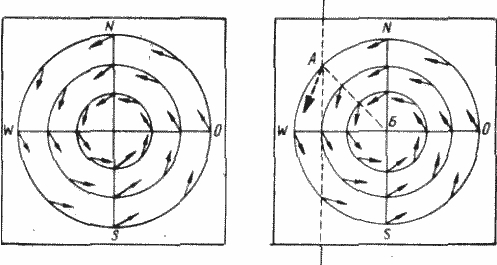
\includegraphics[width=\linewidth]{PP-23.jpeg}
  \caption{Штормовая картушка}
  \label{fig:pp23}
  \small
  \centering{}
\end{figure}

Если судно оказалось на периферии движущегося тропического или
развитого глубокого циклона (что достаточно уверенно можно определить
на основании описанных признаков и методов), то, чтобы выбрать
наилучший путь для расхождения с наиболее опасными районами циклона,
нужно установить, какая часть циклона надвигается на судно. Иначе
говоря, какое положение занимает судно относительно движения центра
циклона.

Для этого рекомендуется непрерывно вести наблюдения за изменением
ветра и давления. Если ветер в течение 1--3~ч поворачивает вправо и
несколько усиливается, то на судно надвигается правая половина циклона
(по направлению его движения), если влево "--- левая половина. Если ветер
не меняет своего направления, а сила его увеличивается и давление
падает, то судно находится на линии движения центра циклона и
приближается к нему.

Определив направление на центр циклона и часть циклона, которая
надвигается на судно, необходимо лечь на такой курс по отношению к
центру циклона, который уводил бы судно с линии его движения. Чтобы
принять решение о выборе пути уклонения, проложите путь движения
циклона на карте на основании данных, полученных из прогноза или с
помощью штормовой картушки.

Следует придерживаться следующих курсов судна относительно ветра (при
плавании в северном полушарии): при приближении правой половины
циклона лечь на курс бейдевинд правого галса, приводя постепенно все
круче и круче к ветру; при приближении левой половины циклона "--- на курс
бакштаг правого галса. Находясь на самом пути центра тропического
циклона, лечь на курс фордевинд.

При плавании в южном полушарии необходимо: в случае приближения судна
к правой половине циклона лечь на курс бейдевинд левого галса и
приводить против ветра, а при приближении левой половины циклона "---
на курс бакштаг левого галса, находясь на пути центра циклона, лечь на
курс фордевинд.

Во всех случаях надо придерживаться указанных курсов до начала подъёма
давления.

\begin{figure}[htb]
  \centering{}
  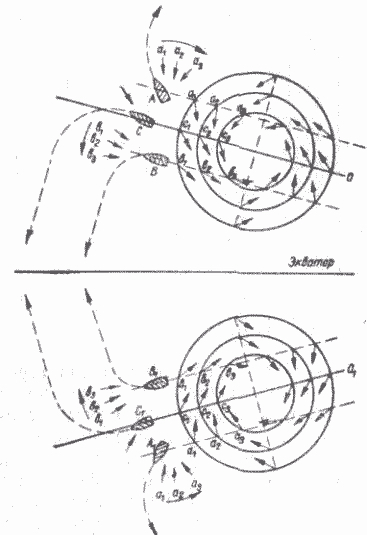
\includegraphics[width=\linewidth]{PP-24.jpeg}
  \caption{Схема уклонения от тропических циклонов}
  \label{fig:pp24}
  \small
  \centering{}
\end{figure}

\subsubsection{Уклонение судов от штормовых районов глубоких циклонов}

Положение судна в любой из областей циклона определяют по той системе
ветров, которая характерна для каждой части (\rris{pp25}). Когда
определены направление на центр циклона и сектор, где находится судно,
необходимо, как и при уклонении от урагана, лечь на такой курс,
который уводил бы судно от линии движения центра циклона.

\begin{figure}[htb]
  \centering{}
  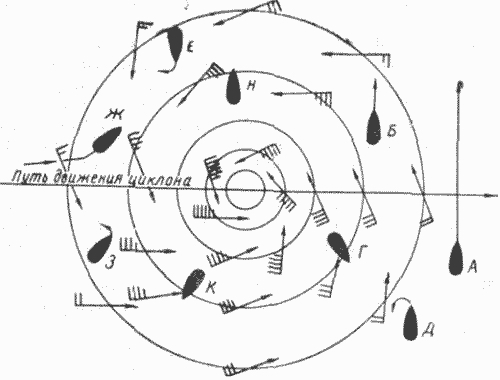
\includegraphics[width=\linewidth]{PP-25.jpeg}
  \caption{Уклонение судов от штормовых районов хорошо развитых глубоких циклонов}
  \label{fig:pp25}
  \small
  \centering{}
\end{figure}

Предположим, что судно находится в точке \textit{А}, около линии
движения центра. Будучи уверенными в том, что линию движения центра
циклона удастся пересечь перед ним, нужно по возможности держать курс
перпендикулярно линии движения циклона. В северном полушарии ветер
будет с правого борта судна (в южном с левого). Судно, находящееся в
южном секторе циклона, например, в точках \textit{Г} и \textit{К},
идёт (в северном полушарии) так, чтобы ветер был справа по носу.

Если невозможно выполнить указанный маневр, судно должно удерживаться
против волны, работая машиной. Если циклон находится перед судном и
оправа от него (положение \textit{Д}), следует лечь на обратный курс.

Судно, находящееся в передней части левой половины циклона, например,
в точке \textit{Б}, должно по возможности удалиться от центральной области
циклона курсом, перпендикулярным линии движения циклона, ветер при
этом должен быть в северном полушарии с правого, а в южном с левого
борта. Если такой курс держать невозможно, нужно, чтобы ветер в
северном полушарии был справа по корме судна (в южном слева) и полным
ходом идти вперёд.

Судну, находящемуся на периферии тыловой части циклона, в левой его
половине (положение \textit{Е}) или приближающемуся к этому району, следует
повернуть вправо и оставить циклон с левого борта.

Судну, догнавшему циклон (тропический или глубокий обычный),
целесообразно лечь в дрейф и подождать его ухода (положение \textit{Ж}).

Судно, приближающееся к тыловой правой половине циклона или
находящееся на её периферии (положение \textit{3}), должно отвернуть влево и
оставить циклон с правого борта.

Во всех случаях при выходе судна из циклона необходимо следить прежде
всего за ходом атмосферного давления. Заметное повышение давления "---
первый и надёжный признак того, что судно удаляется от центра
циклона. При плавании вблизи островов судно может укрыться от шторма с
противоположной стороны ближайшего острова. Но необходимо помнить, что
при прохождении центра циклона через место стоянки судна штормовой
ветер обычно после кратковременного (около 1--2~ч) ослабления или
затишья изменяет направление на противоположное, вследствие чего
судно может быть выброшено на мель.

\subsection{Туманы}

Несмотря на оснащённость судов радиолокаторами, туманы и в настоящее
время представляют большую опасность для судовождения. На морях и
океанах туманы чаще всего образуются в результате адвекции
(горизонтального перемещения) тёплого и влажного\index{влажность воздуха} воздуха над
относительно холодной водной поверхностью (\rris{pp26}). Эти туманы
отличаются значительной вертикальной мощностью, большой
продолжительностью существования (до нескольких суток подряд), большим
районам охвата, подвижностью, внезапностью появления.

\begin{figure}[htb]
  \centering{}
  \includegraphics[width=\linewidth]{PP-26.jpeg}
  \caption{Адвективный туман над морем}
  \label{fig:pp26}
  \small
  \centering{}
\end{figure}

Рассеиваются адвективные туманы обычно в случае резкого изменения
направления ветра, при котором в данный район распространяются более
тёплые или холодные и относительно менее влажные массы воздуха.

Туманы образуются обычно в умеренных и полярных широтах, где
происходят частые и значительные колебания температуры воздуха и где
существуют резко выраженные холодные морские течения, близко
граничащие с тёплыми. В тропических широтах туманы наблюдаются очень
редко.

Если сравнить схему поверхностных морских течений с картами
распределения туманов на морях и океанах, сразу можно обнаружить, что
наибольшая повторяемость туманов приходится именно на районы холодных
течений. Воздух над морем всегда содержит много влаги и часто бывает
близок к насыщению, поэтому достаточно сравнительно небольшого его
охлаждения, чтобы он стал полностью насыщенным. Это может произойти в
том случае, если воздух проходит над поверхностью холодных вод. Поэтому
районы холодных течений и холодных вод вообще характеризуются весьма
частыми туманами.

В Атлантическом океане весьма обширным <<туманным районом>> является
область около Ньюфаундленда, где воздушные массы, нагретые и
увлажнённые над Гольфстримом, при юго-восточных и южных ветрах
перемещаются затем на поверхность холодного Лабрадорского
течения. Аналогичным путём образуются туманы на Тихом океане в районах
действия холодных течении (Ойя-Сио, Приморского, Севере Корейского и
др.) На наших морях туманы особенно часто образуются во время летнего
муссона с апреля по август (особенно в июне ч июле) при юго-восточных
и южных ветрах Над тёплыми течениями туманы почти не наблюдаются.

Возникнув над поверхностью холодного течения, туман распространяется
затем на соседние районы. Например, если туман возник под влиянием
юго-восточных и южных ветров, то частым туманам могут быть подвержены
районы, лежащие к северу и западу от холодного течения. Туманы здесь
появляется при устойчивых ветрах, дующих из района его образования, и
сохраняются все время, пока удерживаются ветры данного
направления. Интенсивность приносимого тумана зависит от температуры
подстилающей поверхности данного района. Чем она выше (по сравнению с
температурой холодного течения), тем в большей степени будет
ослабевать приносимый туман.

Обычно в таких случаях туманы имеют суточный ход: наиболее густыми
бывают в ночные и утренние часы, днем ослабевают или временно
рассеиваются. Если условия подстилающей поверхности неоднородны,
например, имеются районы поднятия на поверхность холодных глубинных
вод и мелководные районы с большим местным прогревом поверхности воды,
то туман будет располагаться пятнами. Эти явления более резко выражены
при слабых ветрах и менее "--- при сильных.

Исчезновение морского тумана может быть внезапным "--- сразу после
прохождения холодного фронта или постепенным "--- по мере перехода тумана
в дымку видимость постепенно улучшается.

На морских побережьях туманы образуются при медленном поступлении с
моря влажного\index{влажность воздуха} и тёплого воздуха на холодную поверхность суши, что
обычно происходит осенью, зимой и весной. По ровной местности,
например, по долинам рек, туман распространяется беспрепятственно и
может проникать свыше 100~км в глубь суши. Но это обычно происходит
ночью и утром, когда поверхность почвы охлаждена. Днем же туман,
попадая на берег, быстро рассеивается.

Горные хребты служат препятствием для распространения тумана. С
наветренной стороны туман усиливается. Иногда высокие берега
покрываются туманом, в то время как у поверхности воды он
отсутствует. Это объясняется следующим. Охлаждение, испытываемое
воздухом над поверхностью, может оказаться недостаточным для
образования тумана. Поднимаясь по склонам береговых гор, воздух
дополнительно охлаждается и достигает состояния насыщения. Но
спускаясь по подветренным склонам гор, он быстро нагревается, и туман
обычно исчезает. По этой причине распространение туманов с моря на
гористом побережье имеет весьма неравномерный характер.

В некоторых бухтах\index{бухта} и заливах, закрытых со стороны моря высокими
горами, туман встречается очень редко. В то же время в районах,
сравнительно далёких от моря, но не отдалённых от него горами, туманы
часты.

Кроме адвективных туманов, при отрицательной температуре воздуха над
морем нередко образуются туманы испарения, или так называемое <<парение
моря>>. Это происходит, когда температура воздуха ниже температуры
поверхности моря на 10\grC и более. Высота туманов испарения обычно не
превышает 3--5~м над водной поверхностью.

Фронтальные туманы (туманы осадков) образуются в случае, если холодный
воздух под слоем слоисто-дождевых облаков достаточно влажен, а
выпадающие капли дождя, испаряясь, усиливают степень насыщения воздуха
водяными парами. Наблюдаются фронтальные туманы в районе окклюзии или
впереди тёплого фронта, в полосе шириной в несколько десятков
километров.

Радиационные туманы, образующиеся на берегу и суше при сильном ночном
охлаждении подстилающей поверхности, на море, как правило, не
образуются, так как охлаждение воды и воздуха над морем в течение ночи
невелико. Признаки появления и исчезновения туманов на море следующие.

\p{289} Туманы следует ожидать, если после более или менее
продолжительной холодной погоды наступает потепление. Они могут
держаться довольно долго. Особенно большая вероятность появления
туманов, если потепление началось вечером или ночью при слабых ветрах.

\p{290} Значительный рост относительной и абсолютной влажности\index{влажность воздуха} воздуха
благоприятствует образованию тумана.

\p{291} Если при ясном небе наблюдаются признаки приближения тёплого
фронта, следует ожидать появления тумана.

\p{292} В средних широтах появление туманов над районами холодных течений
в западных частях морей и океанов в северном полушарии более вероятно
при ветрах юго-восточных и южных румбов, в южном
полушарии "--- северо-восточных и северных румбов; в восточных частях: в
северном полушарии при ветрах юго-западных и южных румбов, в южном "---
северо-западных и северных.

\p{293} В средних широтах появление туманов маловероятно в северном
полушарии при ветрах северных румбов, в южном "--- южных румбов; ранее
образовавшийся туман при переходе ветра на эти румбы скоро исчезает.

\p{294} Если во время тумана пойдёт ливневый или обложной дождь, то туман
при этом ещё более усиливается, но с окончанием дождя скоро исчезает
или значительно ослабевает, даже при прежнем ветре.

\p{295} Днем в прибрежной зоне моря (в заливах, бухтах\index{бухта} и т.\=,п.) и на
берегу туман иногда рассеивается вследствие прогревания воздуха, но
если над морем у горизонта удерживается полоса тумана, а ветер с моря
сохраняется прежний (т.\=,е. тот, при котором туман возник), то
вечером или ночью туман появится и в прибрежной зоне моря, и на берегу

\p{296} При сплошной облачности туман менее вероятен, чем при ясном
небе, в особенности на побережье.

\p{297} Высокий туман продолжителен, тонкий рассеивается вскоре после
восхода солнца.

\p{298} На берегу, если в вечерние часы температура воздуха близка к
точке росы (выше её не более чем на 3--4\grC), то при ясной ночи к утру
можно ожидать появления радиационного тумана, который рассеется при
восходе солнца. При данных условиях образованию тумана будет
способствовать наличие слабого ветра от 0,5~до 5\speedms.

\p{299} После дневных или вечерних гроз, вызывающих похолодание, ночью
и к утру, а иногда и днем при слабом ветре можно ожидать появление
туманов.

\p{300} Перед ночной грозой вечером туман не появляется: если появляется,
то быстро рассеивается.

\p{301} Находясь в море и имея данные о распределении температуры
поверхностной воды, нужно выбирать, если возможно, наиболее высокие
температуры "--- там вероятность тумана меньше.

\p{302} Если утром роса или иней "--- тумана в ближайшие 12~ч не будет.

\subsection{Признаки погоды на отдельных морях}

Как было сказано, кроме общих признаков, имеются и специальные,
характерные для конкретного географического района. Найти такие
признаки можно в различных навигационных пособиях.

\subsubsection{Чёрное море}

Среди ветров особой известностью выделяется новороссийская
бора\footnote{Кроме Новороссийска, более слабая бора бывает на Новой
  Земле, Адриатическом море, на берегах Антарктиды, на озере Байкал и
  в других местах.}\index{бора}. Она вызывает самые опасные шторма на
северо-востоке Чёрного моря, особенно в районе побережья Анапа "---
Новороссийск "--- Туапсе. Новороссийская бора "--- очень сильный
холодный северо-восточный порывистый ветер, дующий с невысоких горных
склонов. Наиболее силен он в Цемесской (Новороссийской) бухте\index{бухта}. Здесь
сильно охлаждённый материк круто обрывается к тёплому морю.

Бора бывает при антициклоне в холодном воздухе над южными районами
европейской части России и при циклоне над юго-восточной частью
Чёрного моря. При этом создаются большие горизонтальные градиенты
давления, вследствие чего поток воздуха низвергается через Мархотский
перевал в Новороссийскую бухту\index{бухта} со скоростью урагана, вызывая сильное
волнение моря с крутой волной и при отрицательных температурах создаёт
обледенение судов и портовых сооружении.

Были случаи, когда суда тонули в бухте\index{бухта} под тяжестью образовавшегося на
них льда. В среднем Новороссийская бора за год наблюдается 46 раз,
чаще всего в период с ноября по март. Из них больше половины бывает со
скоростью ветра выше 20\speedms. Наибольшая скорость ветра 40\speedms
и более, температура воздуха при этом может понижаться до минус
15--18\grC и ниже.

Бора продолжается непрерывно в течение 1--3 суток, иногда до недели. Её
распространение в сторону моря не превышает 5--6 миль.

Местные признаки наступления, ослабления и прекращения новороссийской
боры следующие:
\begin{itemize}
\item Появление белесоватого облачного вала над хребтом Варада и его
  сползание по склонам гор в сторону моря. Бора начинается, когда
  облачный вал спустится примерно до половины склона гор.
\item Если облачные массы оторвались от Мархотского перевала и быстро
  смещаются в юго-западном направлении "--- это признак того, что бора в
  Новороссийске начнётся через 2--3~ч и даже раньше.
\item Резкое ослабление северо-восточного ветра в Новороссийске при
  сильном на Мархотском перевале (о чем говорит удерживающийся почти в
  прежнем положении облачный вал на склоне гор) не указывает на
  окончание боры; ветер вновь усилится через 2--3~ч.
\item Усиление северо-восточного ветра в Новороссийске до 6--7 баллов и
  даже больше при сохранении слабого ветра на Мархотском перевале
  указывает на то, что в Новороссийске скоро не будет ветра.
\item Если надвигается и увеличивается облачность нижнего яруса с юга,
  сопровождаемая осадками и падением давления, то бора прекратится
  через 8--12~ч.
\item Быстрый рост давления в Новороссийске "--- признак начала ослабления
  и скорого прекращения здесь боры.
\end{itemize}
  
В районе побережья Поти с октября по март часто наблюдается очень
сильный феновый восточный ветер, достигающий иногда скорости до
40\speedms и продолжительность до нескольких суток. Этот ветер
наблюдается от реки Супса до реки Ингури, в море он распространяется
до 10~миль от берега. Местное название ветра "--- Потийский калач или
кругляк. Признаки возникновения штормового восточного ветра в районе
Поти следующие:
\begin{itemize}
\item атмосферное давление выше 1015~мбар с равномерным его падением;
\item значительное повышение температуры воздуха и уменьшение
  относительной влажности\index{влажность воздуха};
\item появление перистых и чечевицеобразных облаков над горами;
\item сверхдальняя видимость отдалённых гор;
\item исчезновение низких облаков.
\end{itemize}

Обычно этот ветер усиливается во второй половине ночи и в середине дня
стихает, а к вечеру может усилиться вновь.

В районе Поти также нередко наблюдаются и шквалистые\index{ветер!шквал}\index{шквал} западные ветры,
чаще всего юго-западные и западные, реже северо-западные. Признаки их наступления следующие:
\begin{itemize}
\item появление при фене над побережьем перистых облаков и постепенное
  их уплотнение с образованием облаков среднего яруса "--- признак
  того, что в ближайшие 6---10~ч здесь возникнут шквалистые\index{ветер!шквал}\index{шквал} западные
  ветры и наступит пасмурная погода с осадками;
\item появление зыби на море при ясной погоде, особенно во время фена;
\item сверхдальняя видимость гор;
\item усиление морских течений в районе Поти до одного узла и более
  "--- признак усиления здесь западного ветра до штормового через
  18--24~ч.
\end{itemize}

Признаком усиления этого ветра через несколько часов (3--4) является
заметное повышение уровня воды в Поти.

В апреле и мае при ненормально высокой температуре, малой
относительной влажности\index{влажность воздуха} (сухости) воздуха и падении давления надо
через несколько часов ожидать с юго-запада внезапного сильного шквала\index{ветер!шквал}\index{шквал}.

В районах мысов Тарханкут, Сарыч, Судака, Калиакра, Анапа и в
Керченском проливе при заметном изменении атмосферного давления
наблюдается местное усиление слабых и умеренных ветров до сильных и
штормовых: южного ветра при падении давления, северного "--- при
повышении. При изменении давления в этих районах на 1--2~мбар ветры
могут усиливаться до 6--7 баллов. Усиление распространяется от берега в
море до 5--6~миль, дальше ветры резко ослабевают.

В бассейне Чёрного моря сильные и продолжительные штормы от
направлений северной половины горизонта наблюдаются зимой. Им
предшествуют и сопутствуют резкое понижение температуры и давления
воздуха, выпадение снега, образование туманов, испарения. Скорость
ветра достигает 25--40\speedms.

Штормы от ветров южных направлений на Чёрном море наблюдаются гораздо
реже, и они обычно бывают менее сильными и менее продолжительными, чем
при ветрах северных направлений. Перед началом южного шторма за сутки
и более может наблюдаться сверхдальняя видимость: горы Анатолийского
побережья могут быть видны с Южного берега Крыма.

\subsubsection{Пролив Босфор}

Белые облака, образующиеся над вершинами европейского берега пролива "---
признак скорого наступления северо-западных штормовых ветров. При
этом, если облака начинают сползать по склону гор в сторону пролива "---
значит, скоро появятся сильные северо-западные шквалы\index{ветер!шквал}\index{шквал}, часто
сопровождаемые грозами.

\subsubsection{Эгейское море}

В холодный период года (с октября по март), если горы на островах
скрыты серыми облаками, а небо покрыто низкой облачностью, то скоро
подует сильный ветер. Если небо покрывается облаками, надвигающимися с
юго-запада, давление падает, наблюдаются грозовые разряды, то в
холодный период года нужно ожидать юго-западного шторма. Перед
наступлением северного шторма со шквалами\index{ветер!шквал}\index{шквал} давление заметно
увеличивается и наступает ясная, с хорошей видимостью погода.

\subsubsection{Бискайский залив}

В Бискайском заливе штормы весьма часты. Обычно они наблюдаются с
октября по март и особенно с ноября по февраль. Они сопровождаются
обычно дождливой и ненастной погодой и очень сильным и опасным для
судов волнением. Штормы в Бискайском заливе связаны с прохождением
циклонов, которые чаще всего имеют две траектории: на северо-восток и
восток-юго-восток.

В период с июня по август здесь наблюдаются грозы, которые в южной
части залива сопровождаются сильными шквалами\index{ветер!шквал}\index{шквал}. Признаками наступления
в заливе штормов являются надвигающаяся с запада низкая мрачная
облачность, часто с молниями, и идущая с запада мёртвая зыбь. У южного
побережья залива мёртвая зыбь в сочетании со штилевой погодой,
наступающей после юго-западных ветров, также является верным признаком
приближения шторма.

Характерно также, что чем дольше наблюдаются указанные выше признаки
до наступления шторма, тем сильнее и продолжительнее будет сам
шторм. Возникая обычно с юго-запада, шторм, сопровождаемый осадками и
туманами, поворачивает постепенно на запад или северо-запад и может
продолжаться до нескольких суток подряд. Затем ветер принимает
первоначальное направление. Если по окончании шторма дуют сильные
ветры с юго-запада, сопровождающиеся повышением давления, то можно
ожидать северного ветра и улучшения погоды.

Если обратный поворот ветра с северо-запада на запад или юго-запад
сопровождается значительным падением давления, то надо ожидать скорого
наступления нового шторма.

\subsubsection{Красное море, Аденский и Суэцкий заливы}

В северной части Красного моря и в Суэцком заливе появление перистых
облаков над вершинами гор Синайского полуострова, в то время когда они
видны со стороны южного входа в пролив Губаль "--- признак скорого
возникновения сильного до штормового ветра В этих же районах признаком
скорого появления свежего ветра является дымка на горизонте.

В Суэцком заливе, если дымка покрывает плоскогорья "--- признак скорого
наступления большого шторма. Появлению сухого сильного северного ветра
(хамсина) в Аденском заливе предшествует выпадение обильных дождей в
Йемене.

У северного берега Аденского залива признаком наступления сильного
ветра северного и северо-северо-западного <<белата>> является появление
вечером над берегом тусклой туманной дуги и порывистого ветра,
постепенно заходящего к берегу. В Аденском заливе признаки приближения
циклона от востока и юга "--- гало вокруг луны и солнца, молнии в
восточной части горизонта, шквалы\index{ветер!шквал}\index{шквал} с северо-северо-запада и
северо-северо-востока, мёртвая зыбь, идущая с востока, и падение
давления.

\subsubsection{Порт Кейптаун}

Если вершина горы Лев покрывается белой облачной шапкой — признак
скорого наступления сильного шторма.

\subsubsection{Порт Петропавловск-Камчатский, Авачинская губа}

Признаки усиления северо-западного ветра до штормового следующие:
образование облачной шапки над Вилючинской сопкой, наличие резко
очерченной облачной гряды кучевообразных форм облаков над западной
частью залива.

\subsubsection{Средиземное море}

Изменение направления ветра во время шторма от восточного к западному
служит верным признаком улучшения погоды. Восточные ветры обычно
предвещают здесь штормовую погоду.

\subsubsection{Белое море}

Если на Белом море начинает дуть южный ветер "--- это признак скорого
наступления ненастной погоды.

\subsubsection{Гебридские острова и побережье Шотландии}

Северный штормовой ветер, изменяющий направление на юго-западное при
понижении атмосферного давления "--- верный признак дальнейшего
ухудшения погоды.

\subsubsection{Остров Ньюфаундленд}

Если после западного ветра атмосферное давление начинает медленно
падать, следует ожидать продолжительного восточного шторма.

\subsubsection{Шетландские и Оркнейские острова}

Сильное полярное сияние "--- признак наступления юго-восточного шторма, а
слабое сияние "--- признак наступления хорошей погоды.

\subsubsection{Ботнический залив}

Быстрое падение атмосферного давления, а также заволакивание неба
густыми слоистыми облаками являются признаком приближения циклона и
часто штормового ветра.

\subsubsection{Побережье острова Целебес}

На северном побережье острова, особенно в районе бухты\index{бухта} Манадо, в
период северо-западного муссона наблюдаются штормовые западные ветры,
имеющие местное название <<барат>>. Признак приближения барата "--- тёмный,
свинцовый цвет неба над морем. Температура воздуха при этом падает
обычно до 19\grC вместо обычной здесь 25--27\grC.

\subsubsection{Магелланов пролив}

Видимая на юго-западе белая дуга облаков "--- верный признак
приближающегося от мыса Горн сильного штормового шквального\index{ветер!шквал}\index{шквал} ветра.

\subsubsection{Флоридский пролив}

Часто в этом районе наблюдается штормовой с сильными шквалами\index{ветер!шквал}\index{шквал} ветер,
имеющий местное название <<портер>>. Признаком наступления этого ветра
является падение атмосферного давления и приближение с северо-запада
мощных кучевых облаков при слабом юго-восточном ветре.

\subsubsection{Северный Ледовитый океан}

Снежные струи, переходящие при усилении ветра в позёмок "--- признак
начинающейся пурги. При этом по мере усиления ветра переносимый им
снег поднимается все выше и выше, горизонт постепенно затягивает
снежной дымкой и видимость резко ухудшается.

\clearpage
\subsection{Указатель признаков ожидаемой погоды}
\textbf{Общее ухудшение погоды} 1, 11, 13, 29, 34, 51, 53, 72, 76, 82, 86, 91, 94, 95, 97-99, 103-105, 113, 125-127, 135, 142, 144, 145, 147, 149, 150, 152, 153, 155, 181-187, 192, 198, 201-203, 209, 215, 218-220, 226, 228, 232, 234, 237-250, 253, 254, 258, 260, 261, 268, 269, 275, 277

\textbf{Сохранение плохой погоды} 2, 38, 76, 78, 88, 100, 117, 123,
132, 165, 166, 173, 189, 223, 257

\textbf{Усиление ветра} 1, 2, 4, 6, 7, 11, 13, 14, 16, 18-29, 32, 35,
44, 45, 48, 52-60, 63, 69, 80, 83, 94, 99, 103-105, 108, 113, 115,
126, 131, 144, 145, 177, 178, 194, 204, 216, 218-222, 224, 228, 230,
240, 253, 258, 261, 262, 264, 265-267, 268, 269

\textbf{Осадки} 1, 4, 6, 7, 8, 10, 11, 14, 18-25, 30, 32, 35-38, 47,
49, 53, 64-80, 83, 87, 94, 99, 104, 105, 150, 160, 174, 176, 185, 215,
216, 218-220, 222, 224, 228-240, 243, 244, 246, 253, 254, 256

\textbf{Ливень} 13, 20, 22, 23, 26, 27, 44, 45, 52, 54, 55, 57, 58,
60, 61, 63, 107, 108, 230

\textbf{Грозы,
  шквалы\index{ветер!шквал}\index{шквал},
  смерчи\index{смерч}\index{ветер!смерч}} 8, 16, 22, 24, 26, 27, 28, 44, 52,
55-60, 62, 63, 75, 83, 107, 108, 138, 161, 162, 163, 179, 185, 240

\textbf{Похолодание летом} 14, 19, 22, 24, 35, 44, 59, 64, 124, 257

\textbf{Заморозки (весной и осенью)} 167, 169

\textbf{Мороз} 36, 193, 208, 231

\textbf{Общее улучшение погоды} 33-40, 41, 43, 71, 73, 77, 84, 85, 93,
96, 106, 114, 136, 143, 154, 158, 165, 170, 171, 194, 195, 197, 232,
233, 236, 241, 242, 245, 247, 248, 255, 276

\textbf{Сохранение хорошей погоды} 3, 5, 9, 17, 42, 45, 47, 49, 50,
89, 90, 92-95, 97, 102, 109, 110, 111, 113, 116, 121, 137, 140, 141,
146-148, 151, 159, 164, 180, 186, 188, 190, 191, 200, 205-207,
211-217, 221, 227, 229, 231, 239

\textbf{Прекращение осадков, прояснение} 39, 75, 77, 84, 85, 172

\textbf{Изменчивая погода} 12, 15, 31, 65, 79, 97, 102, 139, 199

\textbf{Приближение тёплого фронта} 1, 4, 21, 32, 38, 48, 76, 81, 94,
106-118, 119, 133, 156, 162, 196-215, 220-228, 232, 259, 273, 274

\textbf{Приближение холодного фронта} 13, 20, 22-24, 45, 59, 75, 108,
120, 134, 179-235, 271, 272

\textbf{Передняя часть циклона} 1, 4, 21, 32, 38, 48, 70, 74, 94, 99,
100, 104, 155, 203, 228

\textbf{Тыловая часть циклона} 40, 41, 42, 129, 145

\textbf{Центр циклона} 105, 130

\textbf{Прохождение левой (внефронтальной) половины циклона} 115, 128

\textbf{Приближение тропического циклона} 122, 278-288

\textbf{Появление тумана} 289-292, 295, 296, 298, 299

\textbf{Исчезновение тумана} 293-295, 297, 300, 301

%%% Local Variables:
%%% mode: latex
%%% TeX-master: "yacht-captain.tex"
%%% End:

\clearpage

\section{Элементы океанологии}

В спортивном мореплавании на больший интерес представляет динамика
моря \--- его волнение, морские течения, приливы и отливы.

\textbf{Волнение.}\index{волнение} Морские волны вызываются
колебательными движениями частичек воды под действием какой\-/либо
внешней силы \--- ветра, прилива, подводного землетрясения (цунами),
изменения атмосферного давления (барические волны\index{барические волны},
или сейши), движения судна. Чаще всего плавающее судно
испытывает действие ветрового волнения и в приливных зонах \---
приливной и отливной волны.

\begin{figure}[!htb]
  \centering{}
  \includegraphics[width=\linewidth]{0124P}
  \caption{Элементы волны и форма ветровой волны}
  \label{fig:124}
\end{figure}

Любая волна имеет следующие элементы (рис.~\ris{124}):
\begin{description}
\item[гребень] \--- часть волны, расположенная выше спокойного уровня;
\item[вершина] \--- наивысшая точка гребня;
\item[ложбина] \--- часть волны, расположенная ниже спокойного уровня;
\item[подошва] \--- наивысшая точка ложбины волны.
\end{description}

Кроме того, каждую конкретную волну характеризуют элементы, имеющие
численное выражение:
\begin{description}
\item[высота (h)] \--- расстояние по вертикали от подошвы до вершины
  волны;
\item[длина ($\lambda$)] \--- горизонтальное расстояние между
  вершинами двух смежных гребней;
\item[крутизна] \--- отношение высоты волны к её длине
  ($k = h / \lambda$);
\item[период ($\tau$)] \--- промежуток времени, за который волна
  проходит свою длину;
\item[скорость распространения ($c$)] \--- расстояние, проходимое
  вершиной волны в единицу времени;
\item[направление распространения ($N\gr$)] \--- угол, отсчитываемый
  по картушке компаса от $N$ (или истинный румб, откуда движутся
  волны).
\end{description}

Линия, проходящая вдоль гребня данной волны, называется
\textbf{фронтом}\index{фронт~волны}, а линия, перпендикулярная фронту \---
\textbf{волновым лучом}\index{волновой~луч}.

Ветровое волнение \--- результат непосредственного действия ветра на
воду в данном месте в данный момент. Ветер изменяет форму волны,
которая отличается тем, что подветренная её сторона значительно круче
наветренной (см. рис.~\ris{124}). Под действием ветра начинается
поверхностное движение воды под ветер, гребень волны опережает
нижележащие частицы воды и рассыпается, образуя пенистые барашки.

Крутизна волны зависит от глубины места: чем меньше глубина, тем круче
волны, тем быстрее они разрушаются, образуя прибои (у берега) и буруны
(на мелководье или на рифах), предупреждая тем самым об опасности.

Высота волны зависит от силы ветра: океанская штормовая волна
достигает 8~м, а ураганная \--- 15\otdo 20~м при длине до 400~м (на
внутренних морях \--- 5 м при длине 20\otdo 40~м). Однако в силу
вязкости воды высота волны имеет предел, после которого она не
увеличивается, какой бы силы ни дул ветер.

На водохранилищах при сильных ветрах волны имеют большую крутизну при
высоте 2~м и более.

Волнение успокаивается, если на поверхности воды находятся водоросли,
битый лёд или <<сало>>, а также при сильном дожде.

Направления волнения и ветра обычно совпадают, но в некоторых случаях
они могут и разниться до четырёх румбов.

Волнение, которое по инерции возникает после прекращения ветра,
называется зыбью. В этом случае волны приобретают правильную
симметричную форму и отличаются большой длиной с очень малой
крутизной. Зыбь в штилевую погоду называется мёртвой зыбью. Обычно она
может служить признаком надвигающегося шторма или сильного ветра,
проходящего стороной.

При встрече волн разных направлений (например, зыби и волны от ветра
другого направления) или отражении волн от стен гидротехнических
сооружений (волноломов, пирсов и т.\=,д.) возникает толчея \---
беспорядочные стоячие волны. На толчее в сильный ветер малыми судами,
особенно тихоходными, управлять плохо, и это надо иметь в виду при
подходе к стенке.

Влияние волнения, особенно штормового, однозначно: оно не только
нарушает нормальный ритм жизни и работы, но в ряде случаев
представляет прямую опасность. Штормовая качка приводит к
перенапряжению всех связей корпуса, особенно деревянного, рангоута и
такелажа. Яхта, попавшая в шторм на мелководье, рискует на большой
волне потерять фальшкиль. Поэтому никакие меры безопасности в
штормовых условиях никогда не будут чрезмерными.

\begin{figure}[!htb]
  \centering{}
  \includegraphics[width=\linewidth]{0125P}
  \caption{Условные знаки течения на карте}
  \label{fig:125}
\end{figure}

\textbf{Морские течения.}\index{течение!морское} Морское течение \---
поступательное перемещение больших масс воды \--- представляет
практическое значение в мореплавании. Обладая направлением и
скоростью, оно оказывает прямое воздействие на направление движения и
скорость судна. В этом смысле важную роль играют ветровые (дрейфовые),
поверхностные и приливо-отливные течения.

Ветровые течения могут быть постоянными в районах господствующих\index{ветер!господствующий}
ветров, чьи скорость и направление меняются мало, и временными
(непериодическими), возникающими при кратковременном действии
ветра. Скорость ветрового течения зависит от силы ветра: 0,5\otdo 0,7
(ветер около 5\otdo 6~баллов) \--- 1,0~уз (в шторм).

\textbf{Поверхностные (навигационные) течения} наблюдаются на глубинах
до 15~м от уровня моря, но могут распространяться и глубже. Они также
бывают постоянными (в океанах \--- Гольфстрим\index{течение!постоянное!Гольфстрим},
Куросиво\index{течение!постоянное!Куросиво}) и
временными. Скорости постоянных течений различны. Они указываются на
навигационных картах и в Лоциях (рис.~\ris{125}).

В плавании все течения учитываются навигационными способами.

\begin{figure}[!htb]
  \centering{}
  \includegraphics[width=\linewidth]{0126P}
  \caption{Уровни и величина прилива}
  \label{fig:126}
\end{figure}

\textbf{Приливы и отливы}\index{прилив}\index{отлив} \---
периодические колебания водных масс \--- заключаются в постепенном
повышении уровня воды до наивысшего и затем постепенным их понижением
до самого низкого (рис.~\ris{126}). Максимальный уровень воды
называется \textbf{полной водой}\index{прилив!полная~вода},
минимальный, после отлива, \--- \textbf{малой водой}\index{отлив!малая~вода}.
Разность между этими уровнями в одном периоде называют
\textbf{величиной прилива}\index{прилив!величина}.

Это явление возникает под влиянием приливообразующих сил, чья природа
лежит во взаимном притяжении Земли, Луны и Солнца. Они влияют на
подвижную водную оболочку нашей планеты. В значительной степени на
приливы влияет притяжение Луны, расположенной намного ближе к Земле,
чем Солнце. Поэтому сила лунных приливов больше чем в 2 раза силы
солнечных. И хотя эти приливы независимы друг от друга, но,
складываясь, они образуют единый лунно\-/солнечный прилив.

\begin{figure}[!htb]
  \centering{}
  \includegraphics[width=\linewidth]{0127P}
  \caption{Фазовое неравенство приливов}
  \label{fig:127}
\end{figure}

При вращении вокруг Земли Луна в течение лунного месяца
последовательно проходит через четыре фазы (рис.~\ris{127}). На
рисунке видно, что при полнолунии и новолунии приливообразующие силы
совпадают и вызывают максимальные (сизигийные) приливы. Когда же Луна
находится в первой или последней четверти, приливообразующие силы
делятся и возникают минимальные (квадратурные) приливы. Такое
неравенство приливов называют фазовым, или полумесячным. Период
изменений приливов равен 14,6~суток.

Различают три формы приливов: суточные, имеющие в период лунных суток
(\hhmm{24}{50}) одну полную воду и одну малую; полусуточные, у которых
за это же время сменяются две полные воды и две малые; смешанные \---
с переменой в течение половины лунного месяца периодов с полусуточных
на суточный, и наоборот.

Наибольшие величины приливов наблюдаются в Атлантическом океане \---
18~м (о.~Фанди), 11\otdo 12~м (у побережья Англии). В Тихом океане они
меньше \--- 7\otdo 8~м (у Аляски) и 13~м (в Охотском море).

Основным пособием по приливам для мореплавателя являются <<Таблицы
приливов>>. Они бывают постоянные и ежегодные. Постоянные <<Таблицы>>
состоят из трёх книг: <<Воды Европейской части СССР и прилегающих к
ним зарубежных районов>>, <<Воды Азиатской части СССР>> и <<Зарубежные
воды>>. В ежегодных <<Таблицах>> зарубежные воды представлены двумя
книгами: <<Атлантический, Индийский и Северный Ледовитый океан>> и
<<Тихий океан>>.

С помощью этих <<Таблиц>> можно вычислить:
\begin{itemize}
\item высоты и моменты полных и малых вод в основных портах на
  заданные сутки;
\item высоты уровня моря в основном порту на любой заданный момент
  между полной и малой водой;
\item время, когда прилив достигает заданной величины.
\end{itemize}

При пользовании <<Таблицами приливов>> следует внимательно
ознакомиться с оглавлением книги и пояснениями к ней.  Приливам всегда
сопутствуют приливо\-/отливные течения \--- периодические
поступательно\-/возвратные движения водных масс, которые зависят в
основном от характера прилива.

Скорости приливо\-/отливных течений в разных бассейнах не одинаковы и
могут быть от 1\otdo 5 (в Белом море) до 0,1\otdo 8~уз и более (в
Тихом океане). Кроме того, приливы активно участвуют в изменении
уровня воды. Это явление сложное и вызывается также сгонно\-/нагонными
ветровыми течениями (классический пример \--- подобные течения в
Финском заливе) и силами гравитации, стремящимися привести частицы
воды в состояние покоя. При плавании крейсерских яхт с большой осадкой
необходимо учитывать эти колебания.

\onecolumn

%%% Local Variables:
%%% mode: latex
%%% TeX-master: "yacht-captain.tex"
%%% End:
